\chapter{Boosted Decision Trees}
\label{chap:Appendix:BDT}


% igual puedo sacarme alguna idea de aquí: https://cds.cern.ch/record/2836731?ln=en
% sacar alguna idea de aquí: https://arxiv.org/pdf/2206.09645.pdf

%\section{Intro}
A boosted decision tree, typically referred by its acronym BDT, is a supervised\footnote{Supervised learning means that the 
data used in the training is labelled.} machine learning (ML) technique used for classification. The analysis presented in this thesis 
uses several BDTs. Both the light-lepton-origin assignment (Section~\ref{sec:ChaptH:Sig:LepAsign}) and the processes
separation (Section~\ref{sec:ChaptH:EventSelection:BDT}) are based on BDTs. This tool is applied in more scenarios 
within ATLAS. In the \btag, for instance, a BDT is trained to discriminate \bjets from light-jets~\cite{ATLAS:2019bwq}. 
During the development of this thesis, two software packages have been used to develop BDTs: TMVA~\cite{TMVAUsersGuide} of ROOT~\cite{Brun:1997pa}
and XGBoost~\cite{Chen_2016}.

Section~\ref{chap:Appendix:BDT:Basics} of this appendix explores the fundamental principles, training procedures, 
evaluation metrics, and practical applications of BDTs. While in Section~\ref{chap:Appendix:BDT:kfold}, the \textit{k}-folding
method for cross-validation is described. Section~\ref{fig:Appendix:BDT:Hyperparams} carefully describes the
hyperparameters that control the training procedure. More details about the metrics and additional considerations
are given in Section~\ref{chap:Appendix:BDT:Concepts}.
The information on the different BDTs presented in Chapter~\ref{chap:Analysis_tH} is complemented in 
Section~\ref{sec:BDT:AdditionalMaterial}. In this section, the metrics of the different folds are presented
separately, the matrices displaying the linear correlation among variables are shown, and the evolution plots
of the different training are introduced.
%Finally, in Section~\ref{sec:BDT:AltModels}, alternative BDT models that have been trained and tested 
%but not used to obtain our results are presented.


%Paragraphs of section intro
%\begin{itemize}
%	\item What is Machine Learning and an MVA method
%	\item what is a BDT
	% source: https://hastie.su.domains/Papers/ESLII.pdf    
		% Chapter Tree-Based Methods
		% Chapter 10: Boosting and Additive Trees
%	\item Uses of the BDT in this thesis: Two different libraries for TMVA ROOT and XGBoost. For XGBoost we have
%	 to convert the data to ¿pandas?¿numpy?
%	\item BDT in comparison to NN	
%\end{itemize}

\section{How does a BDT work?}
\label{chap:Appendix:BDT:Basics}
A BDT is an ensemble of decision trees. Each decision tree is a map of possible results of related decisions. 
A decision tree takes a set of input features and splits input data recursively based on these features. 
This results in a tree structure that resembles that of a flow chart with a decision or split at each node.
The last level of the trees are the so called \textit{leaves} (also known as terminal nodes) and each represents a class label.
An example of a single tree can be seen in Figure~\ref{fig:Appendix:BDT:TreeExample}, where an event is classified in one of the two 
categories following a set of yes/no questions. In this work the BDTs employed are binary, i.e. they separate the dataset into two categories, 
but multiclassifier BDTs could be used as well. In fact for the region definition, multiclassifier BDTs have been
tested but, since the result was not satisfactory, these are not used. 

\begin{figure}
\centering
  \centering
  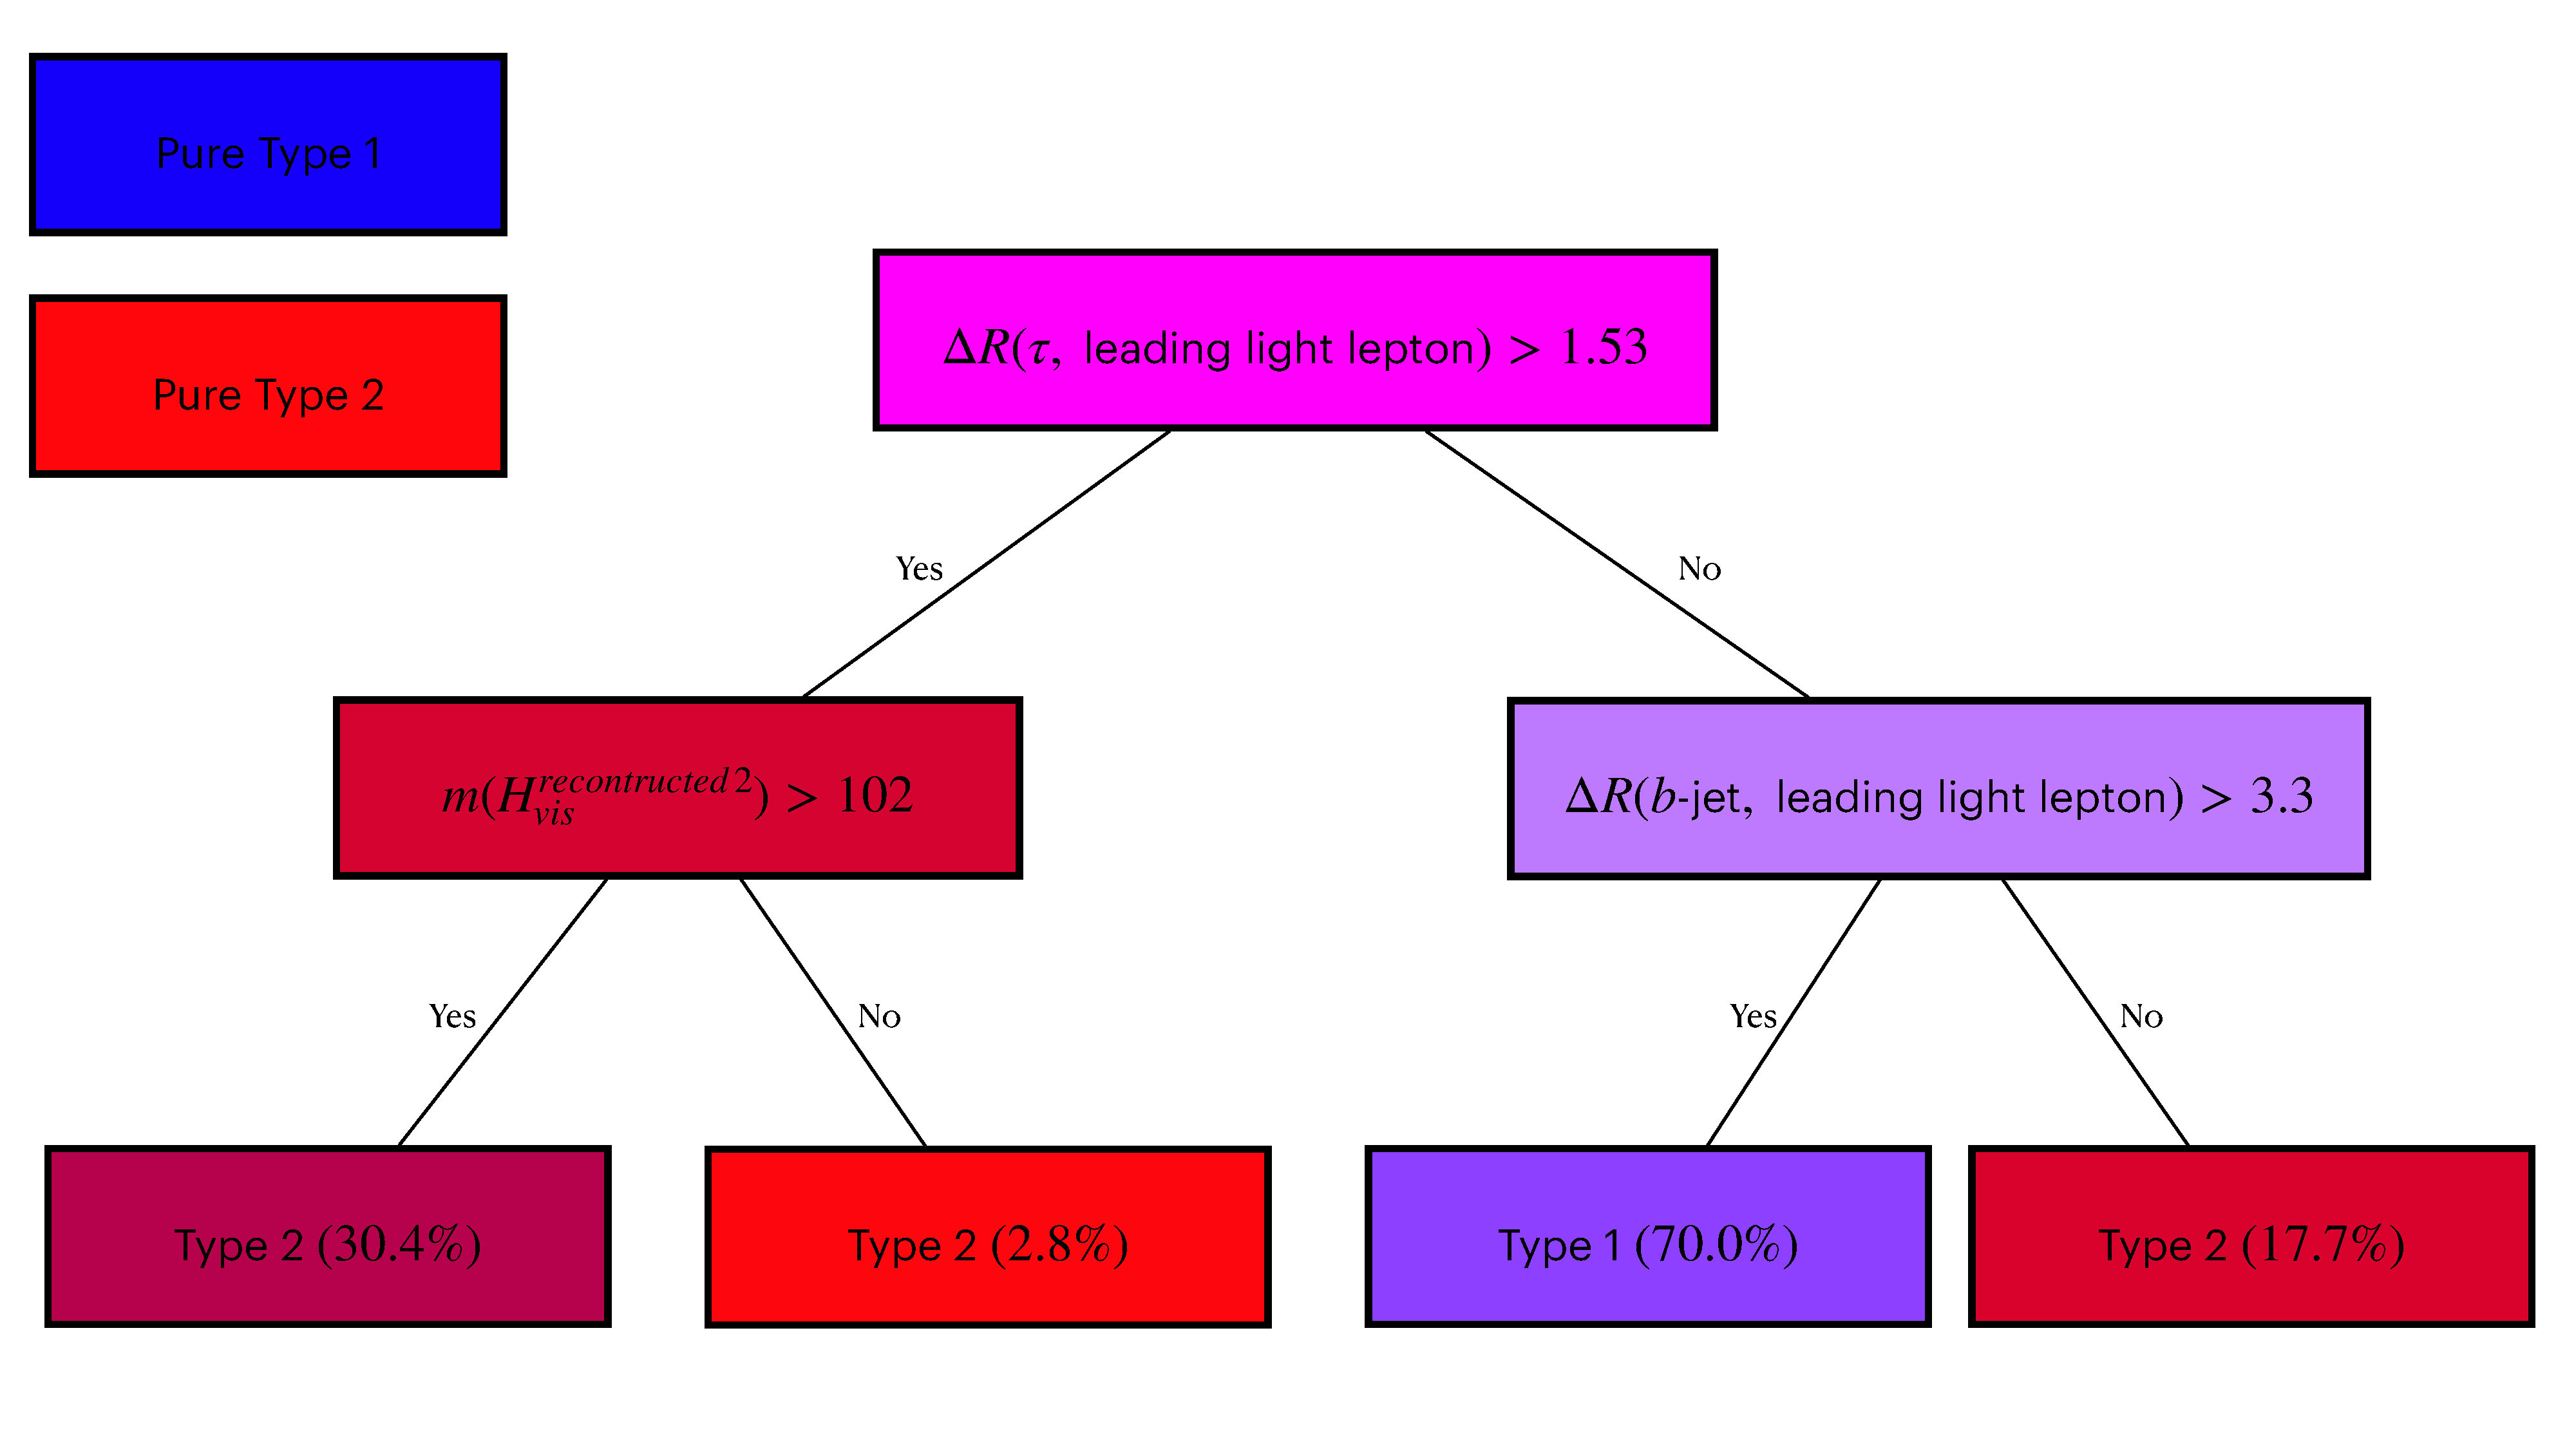
\includegraphics[width=.9\linewidth]{Appendices/BDT/BDT_Assignment_singleTree}
\caption{Example of a decision tree with three nodes. This particular example corresponds to one of the trees in the BDT for the 
light-lepton-origin assignment (see Section~\ref{sec:ChaptH:Sig:LepAsign}). The colour of the boxes represents the 
purity of Type$\,$1 or Type$\,$2 events that arrive at each node. Repeated left/right (yes/no) decisions are taken on 
one single variable at a time until the classification takes place.}
\label{fig:Appendix:BDT:TreeExample}
\end{figure}

Boosting is a technique for turning numerous weak classifiers (trees in this case) into a powerful one. 
Each tree is created iteratively depending on the prior ones. The output of each tree, denoted as $h_{t}(\bm{x})$, 
is assigned a weight, $w_{t}$,
proportional to its accuracy. The ensemble output or prediction is the weighted sum:
\begin{equation*}
	\hat{y} (\bm{x}) = \sum_{t} w_{t}h_{t}(\bm{x})
\end{equation*}
where $t$ run over the trees. 
The $\hat{y}$ is the model prediction of the true label, $y$.
The goal of the boosting is to minimise a regularised objective function:
\begin{equation}
\label{eq:Appendix:BDT:ObjectiveFunction}
	L (x) = \sum_{i} l(\hat{y}_{i}, y_{i})+ \sum_{t}\Omega(f_{t}) \,
\end{equation}

where $l(\hat{y}_{i}, y_{i})=l(f(\bm{x}_{i}|\theta), y_{i})$ is a differentiable convex
loss function which measures the distance between the true label ($y_i$) and its prediction ($\hat{y}_{i}$) on the i$^{th}$ sample.
 The term
$\Omega(f_{t})$ corresponds to the regularisation function, which penalises the complexity of the $t^{th}$ tree, $f_t$.
The $\theta$ in $f(\bm{x}_{i}|\theta)$ are the model parameters. For a BDT, $\theta$ would be the weights
and biases. The $\bm{x}_i$ are values for the input 
variables for the i$^{th}$ sample, while $y_{i}$ denotes the target variable real value. 
The regularisation term $\Omega(f_{t})$ term helps to smooth the final learnt weights to avoid
over-fitting. %There are several types of loss functions such as Huber, Least Squares, Absolute Deviation, etc

The tree ensemble model in Equation~\ref{eq:Appendix:BDT:ObjectiveFunction} cannot be optimised using 
traditional optimisation methods in Euclidean space. 
Instead, the model is trained in an additive way so that the objective function to minimise is:
\begin{equation}
\label{eq:Appendix:BDT:ObjectiveFunction_alternative}
	L^{(t)} =  \sum_{i}^n l(y_i, \hat{y}_i^{(t-1)} + f_t(\bm{x}_i)) + \Omega (f_t) \,.
\end{equation}

There are several types of boosting for BDTs. Some of the most common are AdaBoost, Gradient Boosting and XGBoost. 
The latter, which stands for ``eXtreme Gradient Boosting'', is used 
for region definition and its details can be found in reference~\cite{Chen_2016}.
Boosting can significantly improve performance compared to that of a single tree and stabilise 
the response of the decision trees to fluctuations in the training sample.

%\pablo{Para evaluar la log loss usamos la función log\_loss de sklearn: \url{https://scikit-learn.org/stable/modules/generated/sklearn.metrics.log_loss.html}}


\subsection{Training}
For a supervised ML algorithm, the process of training means to learn or determine optimal values for all the weights within the model. 
To achieve this, the algorithm takes the labelled data and fits the model. In the case of signal discrimination, for instance,
the ML model takes the MC samples, where all the events are labelled. %either as signal or background events. 
%A renormalisation of the data can take place if desired. 
Within the data, the model also requires 
a set of variables that have some power to discriminate between the selected categories. 
The variables used for training are referred as input features. 
A condition on one discriminant variable
is set on each node of the BDT to split the phase space into two parts.
The training aims to find the optimal cut in each node so that after it
the separation between the categories is maximised. %In our example one category is enriched in background and the other in signal.  
This is done in a loop over all discriminating variables and trying to test as many as possible values for each cut 
(the default in TMVA is trying 20 values for each variable). %The best splitting in defined on the basis of the splitting index,
%which works as a mesure of inequality because we want to measure the inequality between the two categories in each split node. 
%A low splitting index value means a high inequality between the classes, i.e. high purity.
%There ara several splitting indices like the gini index, the cross-entropy, misclassification error, statistical significance and others
%they all have similar performance.
The best cut is defined as the one that yields the highest splitting index difference between the parent node
and the two child nodes (each weighted by the total number of events in the corresponding block). 
The splitting process continues until a stopping requirement is met.
%A single tree is a very weak classifier because it is very sensitive to statistical fluctuations in the training MC sample. 
%To increase the sensitivity power of the tree, a solution is create many of them and take an average output.   



\paragraph{Internal reweighting of events in the training sample}\mbox{}\\
Occasionally, MC generators may provide event weights which may turn out to be extremely small or very high. To avoid
artefacts, TMVA can renormalise the signal and background training weights internally so that their respective sums of 
effective (weighted) events are equal. By doing this, the performance of the BDT can be improved since some 
classifiers are sensitive to the relative amount of each category (Type$\,$1/Type$\,$2 or signal/background) in the training data.
While for the lepton assignment, this renormalisation does not play an important role (the amount of Type$\,$1 and Type$\,$2 
signal events is similar), for the \tHq signal discrimination the signal sample in the training test requires reweighting.

Another case of internal reweighting is when negatively-weighted events are present in the training sample and 
the absolute value of the weight is used instead. More details about the problems associated with negatively-weighted
events in the training sample of a BDT can be found in Section~\ref{chap:Appendix:BDT:NegWeigts}.

\subsubsection{Loss functions}
The loss function, also referred to as the error function, is used to evaluate 
the quality of predictions by measuring the deviation between estimated values and 
their corresponding true values during a specific iteration of the model. It penalises 
prediction errors and plays a crucial role in supervised ML models.

%The definition of the loss function, denoted as $l(y_{n}, f(\bm{x}_{n}|\theta))$, may 
%vary depending on whether the model is designed for regression or classification tasks. 
%In the context of this analysis, only binary classification BDTs have been used.

%Classification problems include foreseeing a discrete class output. 
%It entails categorising the dataset into distinct categories based on 
%various factors (variables/features) so that when new and unseen data appears 
%it can be classified as well. 

\paragraph{TMVA loss function}\mbox{}\\ 

The TMVA framework offers various options for loss functions that can be used 
for training and evaluating ML models. The choice of the loss function depends 
on the specific task and the nature of the problem being addressed.
When utilising gradient boost, one commonly used loss function in TMVA is the squared-error loss, which measures 
the squared difference between the predicted value and the true value. It can be expressed as: $l(\hat{y}, y) = (\hat{y} - y)^2$.
%\begin{equation*}
%l(\hat{y}, y) = (\hat{y} - y)^2
%\end{equation*}

%For binary classification tasks, TMVA provides different loss functions that encapsulate 
%the notion of misclassification.% One popular choice is the cross-entropy loss, which 
%quantifies the dissimilarity between the predicted probabilities and the true class labels. 
%It is given by:
%\begin{equation*}
%l(\hat{y}, y) = -\left[ y\log(\hat{y}) + (1-y)\log(1 - \hat{y}) \right]
%\end{equation*}

%The most favoured boosting method, AdaBoost, is based on exponential loss, 
%$l(\hat{y}, y) = e^{(-\hat{y}y)}$. However, exponential loss lacks robustness in 
%the presence of outliers or mislabelled data points, causing the performance of AdaBoost to 
%degrade in noisy settings.

For binary classification tasks, TMVA provides different loss functions that encapsulate 
the notion of misclassification. The most popular boosting method, \texttt{AdaBoost},
is based on exponential loss, $l(\hat{y}, y) = e^{(-\hat{y}y)}$~\cite{freund1995decision}.
However, exponential loss lacks robustness in the presence of outliers or mislabelled 
data points, causing the performance of \texttt{AdaBoost} to degrade in noisy settings.


To address this weakness, the \texttt{GradientBoost} algorithm in TMVA allows for the use of 
other potentially more robust loss functions while maintaining the good out-of-the-box 
performance of \texttt{AdaBoost}. In TMVA, the implementation of GradientBoost for classification, 
the binomial log-likelihood loss function is employed:
\begin{equation*}
l(\hat{y}, y) = \ln\left(1 + e^{-2\hat{y}y}\right) \,.
\end{equation*}


%Since the boosting algorithm corresponding to this loss function cannot be obtained straightforwardly, 
%a steepest-descent approach is employed for minimisation. This involves calculating the current gradient 
%of the loss function and growing a regression tree whose leaf values are adjusted to match the mean 
%value of the gradient within each region defined by the tree structure. Iterating this procedure yields the 
%desired set of decision trees that minimises the loss function. It is worth noting that GradientBoost can be 
%adapted to any loss function as long as the gradient calculation is feasible.


\paragraph{XGBoost loss functions}\mbox{}\\ %source: https://machinelearningmastery.com/xgboost-loss-functions/

The XGBoost library provides various loss functions that can be used for different purposes. 
For binary classification, as is the case in the BDTs presented in Section~\ref{sec:ChaptH:EventSelection:BDT},
the \texttt{logistic} loss function has been used. However, there are other available options, such as \texttt{logitraw} and 
\texttt{hinge}.  These different loss functions allow flexibility in choosing the appropriate approach based 
on the specific requirements of the classification problem.
For the tests involving multiclassifiyer BDTs, the \texttt{softprob} loss function was employed. %~\cite{xgboost2022}

For the \texttt{logistic} loss function in XGBoost, the $l$ term in 
Equation~\ref{eq:Appendix:BDT:ObjectiveFunction_alternative} represents the logarithmic likelihood 
of the Bernoulli distribution. It can be formulated as follows:
\begin{equation*}
\label{eq:Appendix:BDT:binaryLogistic_A}
	l = y_i \log[\text{logistic}(\hat{y}_i^{(t-1)} + f_t(\bm{x}_i))] + (1-y_i)\log[1-\text{logistic}(\hat{y}_i^{(t-1)} + f_t(\bm{x}_i))] \,
\end{equation*}
where $\text{logistic}(\hat{y}_i^{(t-1)} + f_t(\bm{x}_i))$ is the probability for the category.  
In an algebraically equivalent manner, it can be written as:
\begin{equation*}
\label{eq:Appendix:BDT:binaryLogistic_B}
	l = y_i [\hat{y}_i^{t-1} + f_t(\bm{x}_i)) - \log(1 + \exp (\hat{y}_i^{t-1} + f_t(\bm{x}_i))]
\end{equation*}

%Additionally, XGBoost offers other loss functions for classification tasks, including:
%\begin{itemize}
%	\item \textbf{binary:logistic}: Logistic regression for binary classification, providing output probabilities.
%	\item \textbf{binary:logitraw}: Logistic regression for binary classification, providing the raw score before the logistic transformation.
%	\item \textbf{binary:hinge}: Hinge loss for binary classification, producing predictions of 0 or 1 instead of probabilities. 
%		The hinge loss is defined as:
%		\begin{equation}
%		l(f(x_i|\theta), y_i) = \max(0, 1-f(x_i|\theta)y_i)
%		\end{equation}
%		% more about hinge https://www.section.io/engineering-education/understanding-loss-functions-in-machine-learning/#loss-functions-for-classification
%		This loss function is commonly used in support vector machines and focuses on maximising the margin between 
%		the decision boundary and the data points.
%\end{itemize}





\subsubsection{Overtraining}
\label{chap:Appendix:BDT:Overtraining} 
% Source https://root.cern.ch/download/doc/tmva/TMVAUsersGuide.pdf
% From page 31 - Cross Validation

Being $f(\bm{x}|\theta)$ a ML model where $x$ are the data points used as input and $\theta$
the tuneable parameters of the model. The function $f(\bm{x}|\theta)$ outputs the prediction of the model.
The parameters $\theta$ of the model are tuned during the training process using a training set 
($\mathcal{T}$). The true output ($y$) of the elements in $\mathcal{T}$.
When successful, the training finds the $\theta$ that performs as good as possible on new, 
unseen, data.

For a given $f(\bm{x}|\theta)$ model, the training error, $\text{err}(\mathcal{T})$, is defined by 
\cite{zimmermann2006statistical}:
\begin{equation}
\label{eq:Appendix:BDT:ErrorOfTest}
	\text{err}(\mathcal{T}) = \frac{1}{N_t} \sum_{n=1}^{N_t} l(y_{n}, f(\bm{x}_{n}|\theta)) 
\end{equation}
where $N_t$ is the number of events used for the training and $l$ the chosen loss function and
$\bm{x}_n$ and $y_n$ are the features and label points in the training set. So, the error function measures the  
error of the model on a group of objects, whereas the loss function deals with a single data instance.

The $\text{err}(\mathcal{T})$ usually decreases as the number of training cycles increases, and it can begin 
 to adapt to noise in the training data. When this happens the training error continues to 
 decrease but the error on the data outside of the training set starts increasing, jeopardising
 the general performance of the model. This effect is the so called overfitting or overtraining.
 

In other words, overtraining occurs when a ML model can accurately predict training examples but is 
unable to generalise\footnote{By generalise is meant that the model recognises only 
those characteristics of the data that are general enough to also apply to some unseen data.}
 to new data.  When overtraining takes place, the ML model has learnt
the details of the training data to an extent in which this knowledge do not reflect the 
behaviour of the test sample.  This results in poor field performance. 

Figure~\ref{fig:Appendix:BDT:Overtrain} shows how an overtrained BDT evolves. 
In Figure~\ref{fig:Appendix:BDT:Overtrain:AUC} can be seen that as the training of the
BDT continues, the ability of the model to classify the events in $\mathcal{T}$ (blue)
improves while for the data in the test sample (orange), it does not. This means that
the model is not generalising properly. 
With the plot of the loss function (Figure~\ref{fig:Appendix:BDT:Overtrain:LogLoss})
can be seen how the error of the test data slightly increases while for the training
samples is strongly reduced. These two evolution plots can be compared to
the equivalent ones presented in Section~\ref{sec:BDT:AdditionalMaterial:Region:Evolution},
where there is no overtrain.


\begin{figure}[h]
\centering
\begin{subfigure}{.475\textwidth}
  \centering
  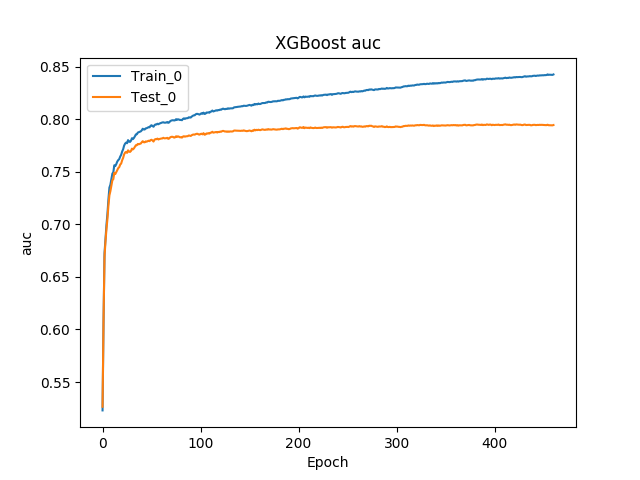
\includegraphics[width=.9\linewidth]{Appendices/BDT/OvertrainingExamples_AUC_SR_tHq_OS}
  \caption{Area under the ROC curve.}
  \label{fig:Appendix:BDT:Overtrain:AUC}
\end{subfigure}%
\begin{subfigure}{.475\textwidth}
  \centering
  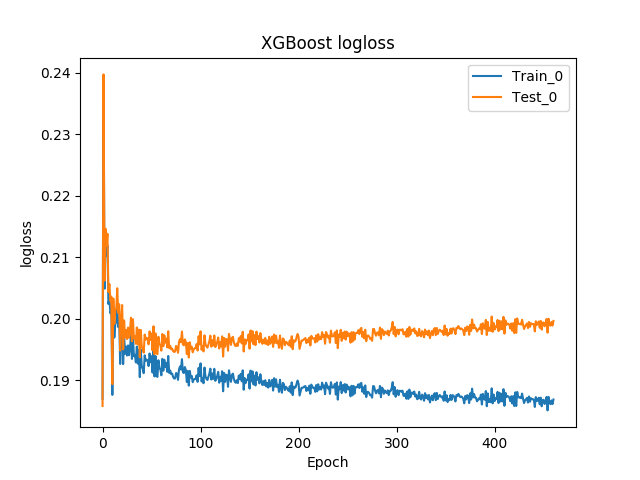
\includegraphics[width=.9\linewidth]{Appendices/BDT/OvertrainingExamples_LogLoss_SR_tHq_OS}
  \caption{Logarithm of the loss function.}
  \label{fig:Appendix:BDT:Overtrain:LogLoss}
\end{subfigure}
\caption{Example of the evolution of the BDT metrics when overtraining occurs. The x-axis shows the training iteration. Observe how the curves for the train and test samples diverge as the training epochs advance.}
\label{fig:Appendix:BDT:Overtrain}
\end{figure}


%When tested on the training sample, overtraining results in an apparent improvement 
%in classification or regression performance over the objectively achievable one, but an 
%effective performance loss when measured on an independent test sample (even though, 
%there is a risk that it can still happen even if we use separate test data).
%Until deployed to real unseen data, there is a danger that
%overtraining will go unnoticed. This makes of overtraining one of the greatest dangers in ML.
%Other names for this phenomenon are overfitting and type III error.

Usually, overtraining is a result of too little data or data that is too homogenous.
It arises when there are too few degrees of freedom because too many model parameters of an algorithm
were adjusted to too few data points.  Not all MVA methods are equally sensible to overtraining.  While Fisher 
discriminant~\cite{fisher36lda} hardly suffers from it, BDTs usually present partial overtraining, owing to their large number of 
nodes. Nevertheless, for the BDTs some countermeasures can be applied to preserve the ability to generalise:

\begin{itemize}
	\item Avoid testing the model on the data used for the training.
	\item The number of nodes in boosted decision trees can be reduced by removing 
		insignificant ones (\textit{tree pruning}). There are two types, pre-pruning and post-pruning
		\begin{itemize}
			\item Pre-pruning: Refers to the early stopping of the growth of the decision tree.
				% In XGBoost "max_depth"
			\item Post-pruning: Allows the decision tree model to grow to its full depth, then removes 
				the tree branches to prevent the model from overfitting.
		\end{itemize}
	\item Cross validation is a powerful technique to use all the data for training at the same 
		time that all the data for testing is employed while avoiding overfitting. This method is
		based in cleverly iterating the test and training split around and it is described on 
		Section~\ref{chap:Appendix:BDT:kfold}.
\end{itemize}
%https://indico.cern.ch/event/294651/contributions/671918/attachments/552028/760654/ESIPAP_MVA130129-BDT2.pdf






%\subsection{Evaluation / Validation}
%The test set should ideally only be used only once to evaluate a model's performance. 
%When a data set is reused, it introduces some bias. Trying out numerous ideas in the 
%early stages of an analysis is a frequent practice to figure out what works and what 
%doesn't. Model selection is the process of choosing the best model from a group of ideas.
%Model selection refers not only to chosen between the types (BDT, Neural Network, k-nearest
%neighbours, SVN, etc) but also about choosing the hyperparameters for a model.




%\subsection{Application}






%%%%%%%%%%%%%%
%   Feature importance algorithm  %
%%%%%%%%%%%%%%
\section{Feature-selection optimisation}
\label{chap:Appendix:BDT:featureOpt}
The optimisation of the list of input variables is divided into two distinct steps: Obtaining the
ranking of the most discriminant variables and removing the features that present high correlations.

The initial step is performed by an iterative method based on the feature ranking provided by the XGBoost package. 
A benefit of the methods that provide a variable ranking is that it allows for interpretability of the results in terms of which physics objects are used.
The XGBoost-ranking tool is based on references~\cite{burges2006learning, wu2010adapting} and it provides a score that 
indicates how useful each feature is in the construction of the BDTs within the model.
It is calculated for a single decision tree by the amount that each attribute split point improves the 
performance measure, weighted by the number of observations the node is responsible for.
After establishing an initial and preliminar set of input variables, each iteration involves the following steps:
\begin{enumerate}
	\item Train the BDT using the current set of variables. 
	\item Rank the input variables according using the XGBoost-ranking tool and
		record various metrics such as the log-loss function and the AUC of the ROC curve.
	\item Drop the lowest-ranked feature from the collection of training variables and go to the first step of the loop.
\end{enumerate}
When all variables have been dropped out, the loop is completed. As a result, we get the information of 
what is the performance of the BDT model depending on which variables have been used.
This allows to understand the actual impact of each variable in the BDT performance
and the effect of removing it from the training.
These steps are schematically illustrated in Figure~\ref{fig:Appendix:BDT:Feature_loop}, where each iteration is depicted.

After doing this, the correlations among variables have to be studied and suppressed. 
The correlation studies for the variables used in BDTs for region definition are presented
in Section~\ref{sec:BDT:AdditionalMaterial:Region:Correlations}.

\begin{figure}[h]
\centering
  \centering
  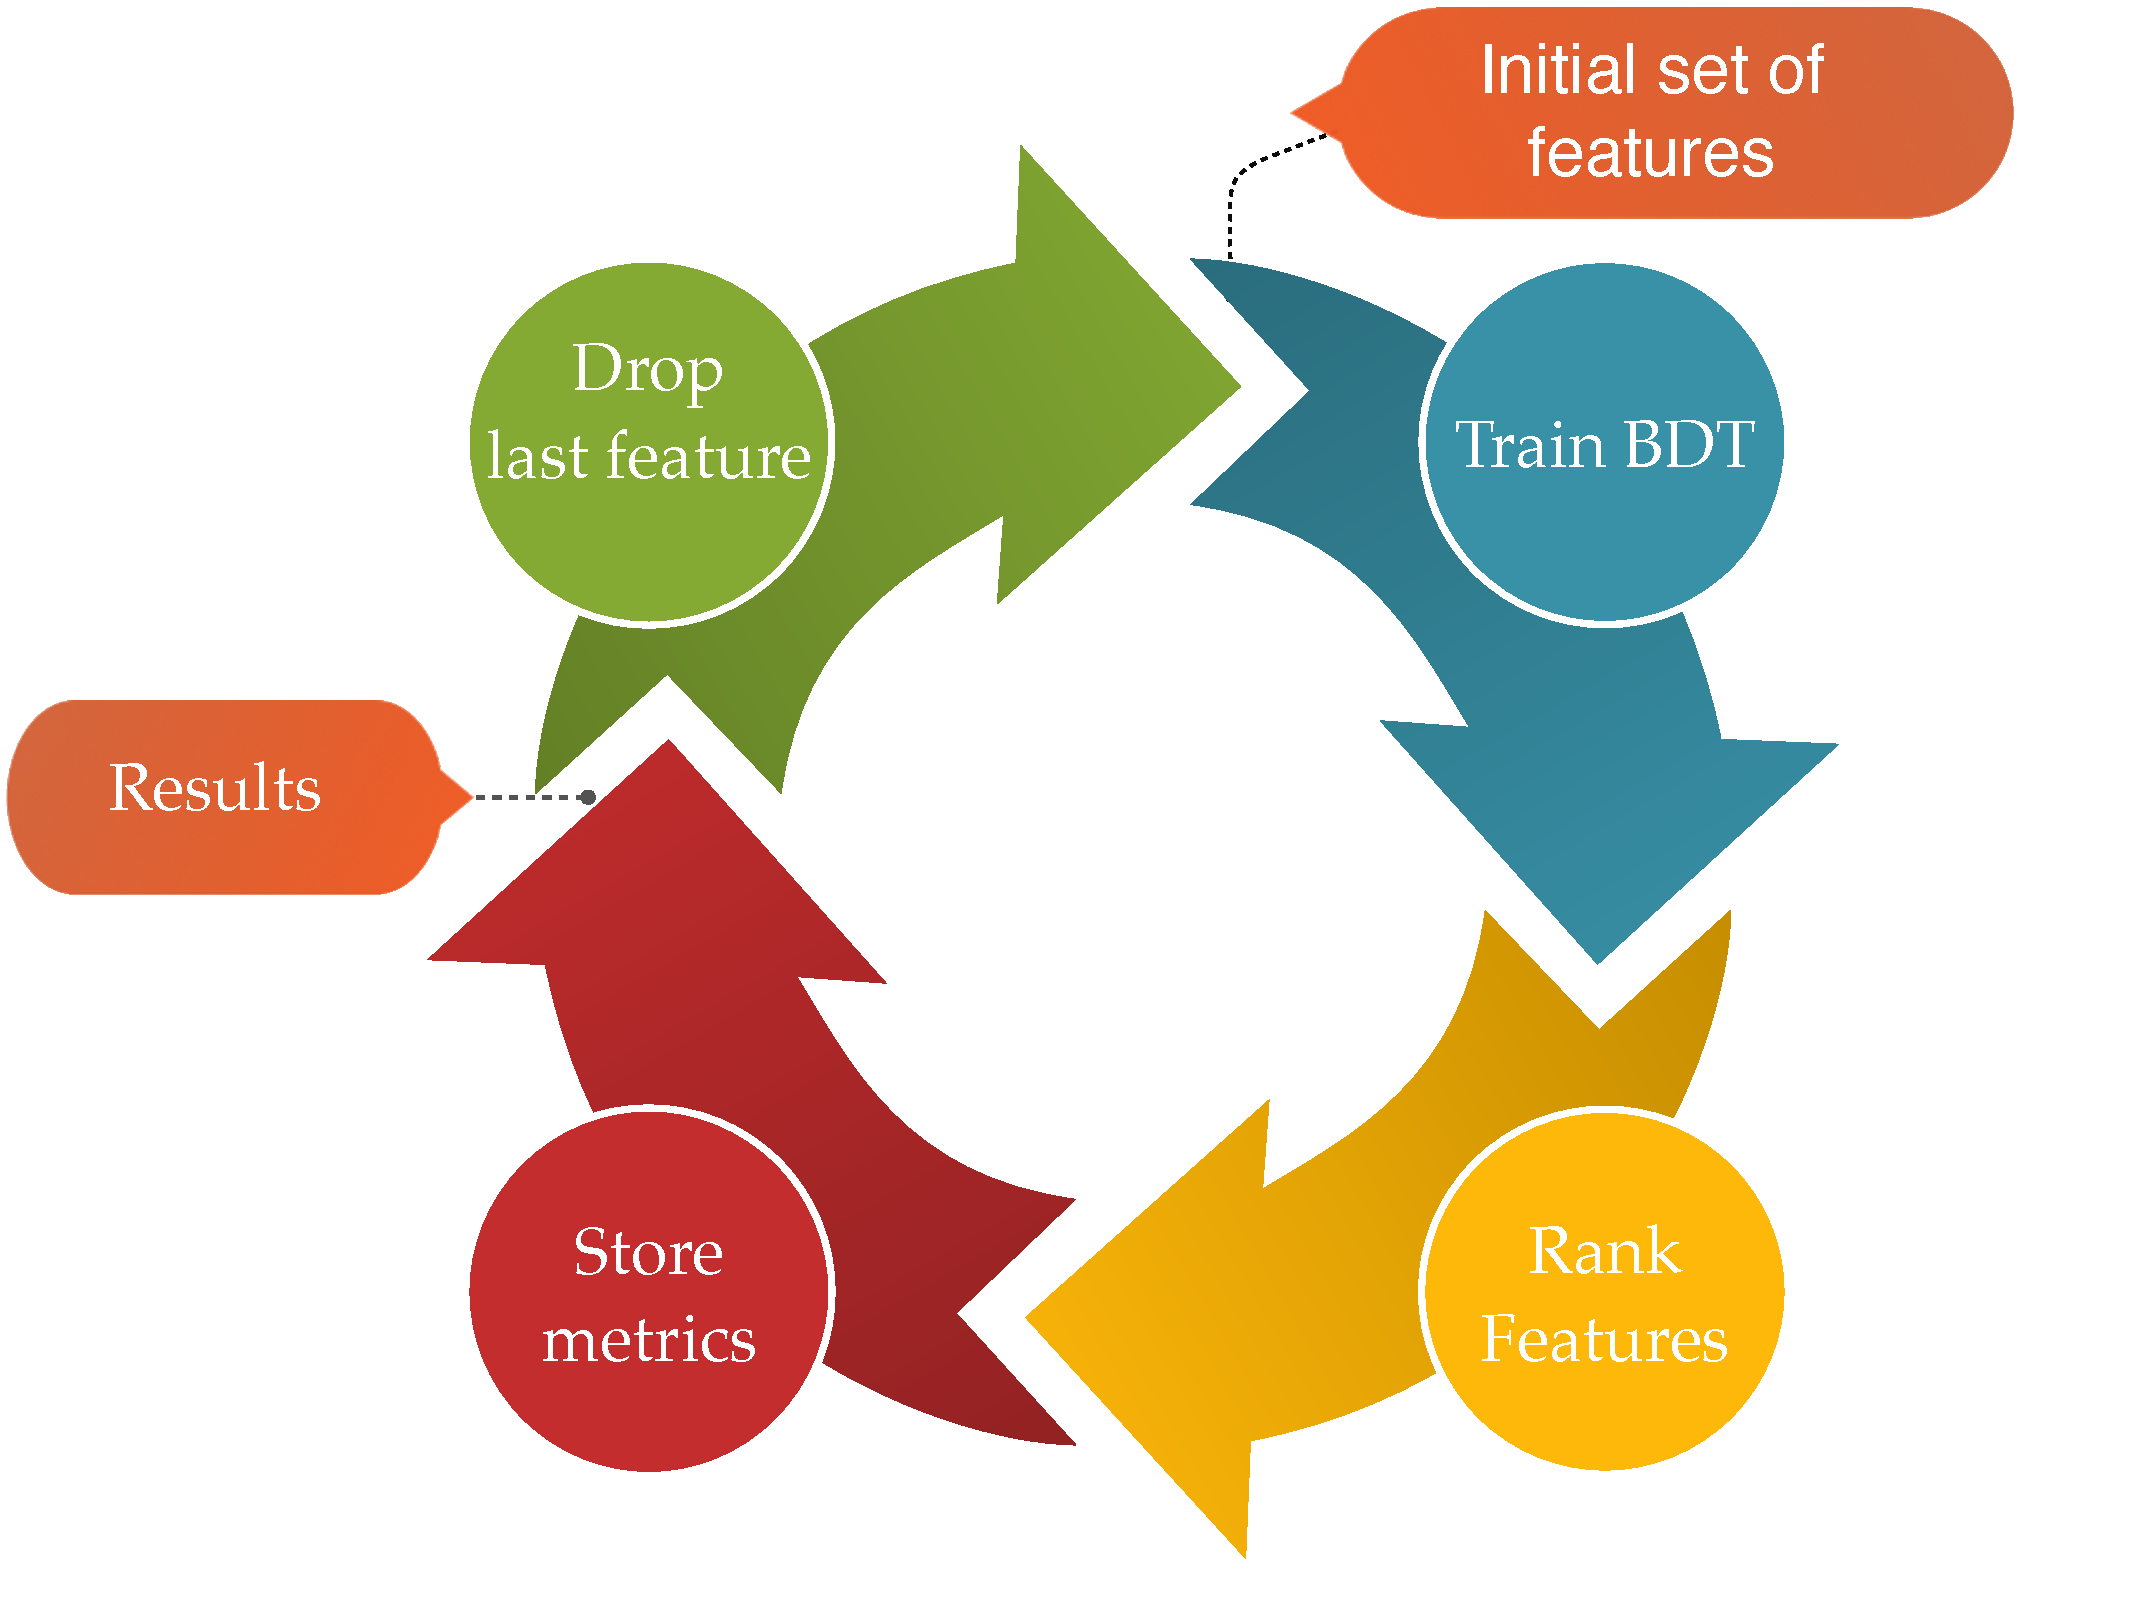
\includegraphics[width=.7\linewidth]{Appendices/BDT/Optimise_feature_english}
\caption{Schematic view of the iterative algorithm method for feature-selection optimisation. The procedure is 
reaped until all features are dropped.}
\label{fig:Appendix:BDT:Feature_loop}
\end{figure}


%%%%%%%%%%%%%%%%%%
%   Negative weights  treatment    %
%%%%%%%%%%%%%%%%%%
\section{Treatment of negative weights}
\label{chap:Appendix:BDT:NegWeigts}
Negatively weighted events can be problematic when training a BDT
for several reasons.
Firstly, BDTs, typically operate under the assumption that data represents probabilities or 
frequency counts. Negative weights violate this assumption, as they do not have a natural 
probabilistic interpretation.
Additionally, negative weights affect the stability and performance of the BDT by 
slowing the convergence model or failing to generalise to new data. 
Negative weights can also distort the process of  correcting the inaccuracies of
the previous trees in the boosting iterations, leading to skewed decision boundaries. 

While for the XGBoost there are no dedicated training options to address this problem,
the algorithm can converge using negatively-weighted events. However, in the
search presented in this thesis, it is prefered to avoid the risks involving the training with
negative events and, hence, either the absolute value of the weight is used
or only the events with negative weights are taken into account in the training
process. Note that these two options are internal reweightings and, after the
training, the event weights are the original ones. %Actually, the testing of the
%model is done using all weights.


For the TMVA case, there are specific options for dealing with events with negative
weights. These are explored below in Section~\ref{chap:Appendix:BDT:NegWeigts:TMVARoot}.


%% TMVA - Neg Weight
\subsection{Negative weights in $\text{BDT}^{\text{Lepton Assignment}}$ }
\label{chap:Appendix:BDT:NegWeigts:TMVARoot}
The TMVA library offers several possibilities to deal with the negatively weighted events.
These are:
\begin{itemize}
	\item InverseBoostNegWeights: It boosts with inverse boostweight.
		This option is not available for gradient boosting.
	\item IgnoreNegWeightsInTraining: This option is the one that is being used and
		as its name suggests, it removes the negatively-weighted events from the training
		sample.
	\item Pray: This option allows to use negative weights in the training but might cause 
		problems with small node sizes or with the boosting. It was tested and the model could not
		achieve stability. 
	\item PairNegWeightsGlobal: This option is still experimental. It takes the negatively 
		weighted events and pairs them with the events with positive weights, annihilating both.
		When using this option the gradient BDT was not able to converge.
\end{itemize}
In the $\text{BDT}^{\text{Lepton Assignment}}$, the selected treatment ignores the negatively weighted events  
in the training. When testing the model, these weights are taken into account.




\section{Cross validation and \textit{k}-folding}
\label{chap:Appendix:BDT:kfold}
Cross validation is a technique consisting of training several ML models on different subsets of the input data
and evaluate these models on the complementary subset of the data. The goal of cross validation is to estimate the
performance of a ML model. Cross validation can identify overfitting or recognise the failure of the model to
generalise a pattern.

One particular method to cross validate is the \textit{k}-folding. It is based on splitting the input data into 
$k \in \mathcal{N}$ equally-sized subsets. Each of these subsets is referred as a fold. With this procedure, the ML model is 
trained \textit{k} times as Figure~\ref{fig:Appendix:BDT:kfold} shows. 
For each train, $k-1$ folds are used in the training set and the remaining non-used fold is the subset 
of data where the evaluation takes place. All folds are used once as test sample and $k-1$ times in the training 
sample. There are no formal rules for the choice of $k$ but typical values are 5 or 10 folds. As $k$ gets larger, the 
difference in size between the training set and the resampling subsets gets smaller. As this difference decreases, 
the bias of the technique becomes smaller. In the analysis
presented in this thesis a $k=5$ is used for both BDTs. 

\begin{figure}[h]
\centering
  \centering
  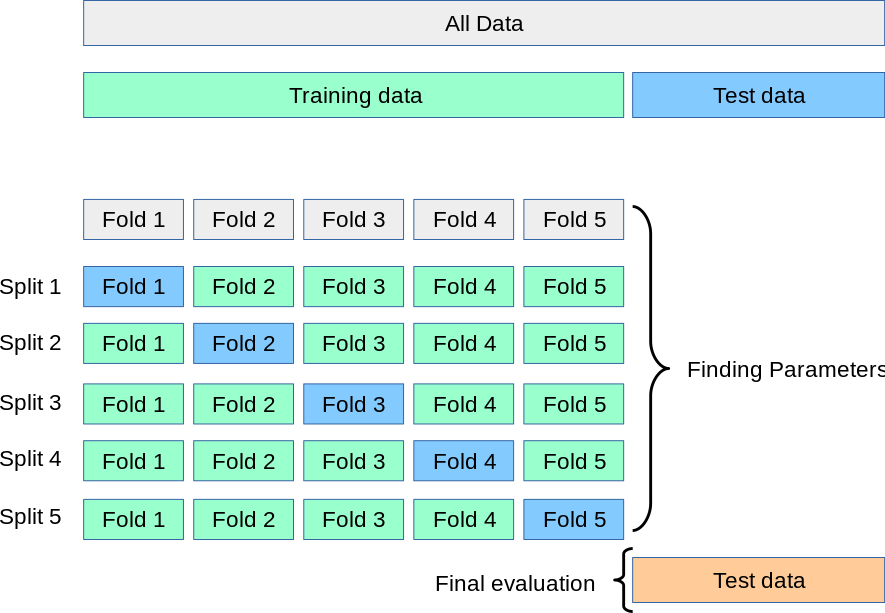
\includegraphics[width=.85\linewidth]{Chapter5_tHq/BDT_generalities/k_folding_cross_validation.png}
\caption{Illustration of \textit{k}-folding method for cross validation using 5 folds. For each model, the 
training folds are presented in green and the test fold in blue. The initial training/test separation is not performed
in our case due to the scarcity of data.} 
\label{fig:Appendix:BDT:kfold}
\end{figure}

The \textit{k}-folding cross validation resample is of particular interest when the data available is limited 
because, by applying this method, all events are used in the training phase.  It generally results in a less biased 
or less optimistic estimate of the model skill than other methods, such as a simple train/test split (although train/test split
is a particular case of \textit{k}-folding using $k=2$).

Note that when the score of the model is applied, each event gets the score that was assigned when
it was used as test event. Not doing this would bias the model.

The expected error for a model $f(x|\theta)$ trained using \textit{k}-folding is:
\begin{equation}
\label{eq:Appendix:BDT:ErrorKFold}
	\text{err}(\mathcal{T}) = \frac{1}{k} \sum_{k} \text{err}(\mathcal{T}_{k}) ,
\end{equation}
where $\text{err}(\mathcal{T}_{k})$ is the error as described in Equation~\ref{eq:Appendix:BDT:ErrorOfTest} for each splits test.
As Equation~\ref{eq:Appendix:BDT:ErrorKFold} shows, an increase in the number of folds would imply more
models to average over and, hence, implying an improvement in the confidence of how consistent 
the $f(x|\theta)$ achieves a given level of performance. However, a larger $k$ would also reduce
the statistical strength of each fold.


When it comes to assigning an event to a fold, there are no particular rules besides trying to ensure that
all the folds represent the general behaviour of your sample and that the size of all folds is
the same. The best way to ensure this is by shuffling the dataset randomly. In this analysis,
the function to split the data sample among the folds is using the event number. The
event number is a categorical variable that assigns a number to each event and it has
no physical meaning. Therefore, using this variable to split the data does not create 
any bias. 

%A problem with \textit{k}-folding is that the estimation
%is not done for the final model, but rather of the average final model.

%There are variations of the \textit{k}-folding cross-validation that are not
%explored in this work. To name a few: Leave-One-Out, 
%stratified or nested cross-validations.



%%%%
% Hyper params
%%%%%
\section{Hyperparameters}
\label{fig:Appendix:BDT:Hyperparams}
Hyperparameters is the term used to refer to the specifications that control\footnote{The prefix ``hyper'' suggest that 
these parameters are on a higher level that modulates the training process.}
 the learning process of a ML algorithm. 

A ML model is defined by its model parameters, which are sat by the process of training. 
To reach some level of intelligence, the process of training a model involves 
selecting the optimal hyperparameters that the learning algorithm will use to learn the
ideal model parameters that accurately map the input variables ($\bm{x}$) to the labels ($y$).
The learning algorithm uses hyperparameters when learning, but these are not included 
in the resulting model. 


\paragraph{XGBoost}\mbox{}\\
In XGBoost, the hyperparameters are classified in three categories: general, booster and task hyperparameters.
For the work developed in this thesis, the parameters related to the boosting of the trees are the ones
that have been optimised. %The process of finding the optimal set of hyperparameters for each model
%is crucial to achieve success. 

\begin{itemize}
	\item General parameters: Refer to which booster its been used. The used option is based on linear functions. % booster = gbtree
	The general parameters also adapt the algorithm to the used device.
	Since the training of the BDTs takes place in ARTEMISA\footnote{ARTEMISA (ARTificial Environment for Machine 
	learning and Innovation in Scientific Advanced computing) is a ML dedicated facility at IFIC. It is composed of 
	several Intel Xeon Platinum CPUs and Tesla Volta GPUs that help to find the optimal configuration for ML algorithms.} 
	facility, it is set GPU.					% device = gpu.     ~\cite{ARTEMISA}
	%Also control the number of parallel threads to be used (set to the maximum in our case). 
	%Whether to train over CPU or GOU
	\item Learning task parameters: Decide on the learning scenario. Specify the learning task 
	and the corresponding learning objective.
	\item Booster parameters: Control the performance of the selected booster. 
	For trees, the most relevant are: 
	\begin{itemize} %https://xgboost.readthedocs.io/en/stable/parameter.html#parameters-for-tree-booster
		\item \textbf{Learning rate}: 
		This tuning parameter %in an optimisation algorithm 
		determines the step size at each iteration while moving toward a minimum of a loss function.
		Figure~\ref{fig:Appendix:BDT:LearingRateTypes} shows the evolution per epoch for the loss function
		depending on the learning rate. This hyperparameter is also known as eta or shrinkage, and it ranges from 0 to 1.
			\begin{figure}[h]
			\centering
  			\centering
  			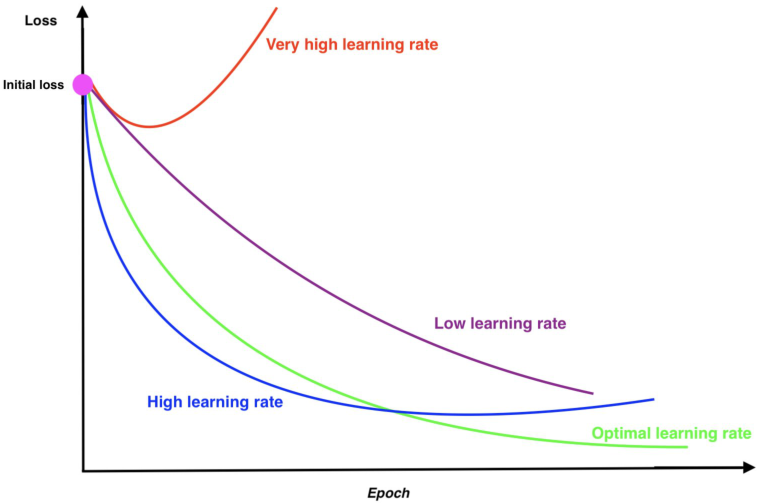
\includegraphics[width=.8\linewidth]{Appendices/BDT/LearningRateTypes}
			\caption{Different loss-function curves versus iteration.
			Learning rate is one of the most important hyperparameters to adjust well during the ML model training. 
			If it s high, it can cause the model to diverge. If it s too low it can slow down the training.}
			\label{fig:Appendix:BDT:LearingRateTypes}
		\end{figure}
		
		\item \textbf{Minimum split loss}: 
		Also known as \textit{gamma} or Lagrangian multiplier.  
		A node is split only when the resulting split gives a positive reduction in the loss function
		and the gamma gives the minimum loss reduction required to make a further partition
		 on a leaf node of the tree. Therefore, the higher the gamma, the more conservative the algorithm
		 will be. The minimum split loss ranges from 0 to $\infty$. 
		 After testing several values for this hyperparameter, it is not being constrained.
		%Reads on gamma hyperparam: https://medium.com/data-design/xgboost-hi-im-gamma-what-can-i-do-for-you-and-the-tuning-of-regularization-a42ea17e6ab6
		
		\item \textbf{Minimum child weight}: 
		It defines the minimum sum of weights of all observations required in a child.
		When the tree partition results in a leaf node with the sum of instance weight less than the value of 
		this hyperparameter, the tree stops partitioning. Higher minimum child weight prevents the model from learning
		too specific relation. So, this is done to prevent overfitting. This tuneable parameter ranges from 0 to $\infty$.
		
		\item \textbf{Maximum tree depth}: It refers to the number of splits in each tree, which controls the complexity 
		of the boosted ensemble. 
		When \texttt{MaxDepth} is set to an integer value greater than zero, the created cell tree will not be deeper than this integer.
		This hyperparameters controls de pre-pruning described in Section~\ref{chap:Appendix:BDT:Overtraining}.
		The maximum depth of a tree is an integer ranging from 1 to $\infty$ but it is rare to have trees
		with depth higher than 10 since XGBoost aggressively consumes memory when training a deep tree.
		In the BDTs for region definition, this hyperparameter is set to either 4 or 5. 
		
		\item \textbf{Scale of positive weight}: When the categories are imbalanced, as it is the case for the signal
		and background in this analysis, the signal sample can be reweighted to have a larger impact. 
		The scale of positive weight is the parameter by which the weights of the target process are multiplied.  
		The typical value to consider is the fraction between positive instances (signal) and negative instances (background). 
		When the BDT is targeting the identification of background processes this hyperparameter can be also used but
		it takes values closer to the unity.
		
		%\item Maximum delta step: 
		
		%\item Subsample
		
		%\item Sampling method
		
		%\item Regularisation
		
		\item \textbf{Tree method}: It alludes to the tree-construction algorithm used in XGBoost.  
		The method used here is the GPU implementation of a variant of the \texttt{LightGBM}~\cite{ke2017lightgbm, Chen_2016}.
		 %faster histogram optimised approximate greedy algorithm.

		
		%\item \textbf{n_jobs}: We use -1
		
	\end{itemize}
\end{itemize}


\paragraph{TMVA ROOT}\mbox{}\\
This section complements the hyperparameter optimisation for the BDT for the lepton assignment
that is described in Section~\ref{sec:ChaptH:Sig:LepAsign:SS:BDT:hyperparameters}.
The TMVA-based BDTs allow to configure the several training hyperparameters.
From those, the ones that have been explored are:
\begin{itemize}
	\item \textbf{Number of trees}: Number of trees in the forest. The more trees, the more complex the 
		model is and, hence, it can learn more. However, the complexity risk is that the BDT can learn 
		the specifics of the training sample, i.e., overtraining.
		% NTrees :: Int
		
	%\item \textbf{Maximum tree depth}: Maximum depth allowed for each decision tree.
	%	The cell tree depth can be limited by using this option. When \texttt{MaxDepth} 
	%	is set to an integer value greater than zero, the created cell tree will not be deeper 
	%	than \texttt{MaxDepth}.  
		% MaxDepth :: Int
			
	\item \textbf{Minimum size for each node}: Minimum percentage of training events required in a leaf node.
	 	The default for classification: 5\%. 
		% MinNodeSize ::  Real
	
	%\item \textbf{nEventsMin}:  Set to 100 by default for binary tree. <-- Depecrated in favour of "Minimum size for each node"
		
	\item \textbf{Number of cuts}: Control the number of cuts tested within 
		a variable in order to find the optimal cut value for a node splitting.
		% nCuts :: Int
		
	\item \textbf{Negative weight treatment}: Controls the approach for handling 
		events with negative weights during BDT training. The TMVA library has options
		to include negative weights in the training by pairing them with positively weighted
		and ``annihilating'' both events. This strategy has been tested but in the end, removing the negative
		events provided the best performance. 
		% NegWeightTreatment :: Str

		
		
	\item \textbf{BoostType}: Type of boosting algorithm. The options are
		% BoostType = Grad
		% source for boost types: https://fhernanb.github.io/libro_mod_pred/gradboost.html and TMVA manual
		\begin{itemize}
			\item \textbf{AdaBoost}: This is the most popular type of boosting algorithm and it
				uses an exponential loss function. Its name comes from ``adaptive boosting''.
				It consists of creating several weak trees, each of them adjusting what the previous one
				could not. This algorithm lacks robustness in the presence of outliers or mislabelled data points,
				which can happen in the lepton-origin-assignment scenario.
			%\item RealAdaBoost
			%\item Bagging
			%\item AdaBoostR2: If this is used, the loss function has to be either
			%	Linear, Quadratic or Exponential.
			\item \textbf{Gradient boosting}: The TMVA implementation of the gradient boost
				 uses the binomial log-likelihood loss function for classification. This algorithm attempts
				 to overcome the problem presented by AdaBoost regarding the outliers or mislabelled data.
				 %The gradient boos creates several trees in sequence and each predictor tree 
				% Grad
		\end{itemize}
		
	%\item \textbf{Learning rate}: Also called shrinkage, it is the learning rate of the GradientBoost 
	%	algorithm. A small shrinkage demands the use of more trees in the BDT but 
 	%	can significantly improve the accuracy of the prediction.
		% Shrinkage :: Here I was using 0.1 and the ROC curves looked terrible. With 0.3 it got better.
		
	
		
		
	%\item \textbf{UseBaggedGrad}: %Only applicable for gradient boosting. 
	%	If used, only a random subsample of the events is used for creating the trees at each iteration.
		%UseBaggedGrad :: Bool
		
	\item \textbf{Use Bagged Boost}: If used, only a random subsample of the events 
		is used for creating the trees at each iteration. The ``bagged sample fraction''
		is the relative size of the bagged sample to the original size of the data sample.
		%Only applicable for gradient boosting. At each iteration it uses 
		%UseBaggedBoost // BaggedSampleFraction.  ::  str/real
	
	% \item \textbf{AdaBoostR2 Loss}: The type of Loss function in AdaBoostR2 can be 
	% 	quadratic, linear or exponential. The default option and the one used 
	%	in quadratic.
	 
	% \item \textbf{BaggedSampleFraction}:
	 	% BaggedSampleFraction 
	
	\item \textbf{Pruning}: 
		Method used for removing statistically insignificant nodes
		in the BDT in order to counteract overtraining.
		For simple decision trees, it is beneficial to first grow the tree to its
		maximum size and then cut back, rather than interrupting the node splitting at an earlier stage.
		However, for BDTs, the best performance is found when small trees (max. depth $\simeq 3$) are
		used rather than big trees with pruning.
		% PruneMethod
\end{itemize}
The learning rate, maximum number of trees, and maximum depth that are explained above 
for the XGboost but these have also been tuned for TMVA.






%%%%%%%%%%%%%%
%   Genetic algorithm   %
%%%%%%%%%%%%%%
\subsection{Hyperparameter optimisation of a BDT with the genetic algorithm}
\label{chap:Appendix:BDT:GA}
A genetic algorithm (GA) is a search heuristic that mimics the process of natural 
selection to find solutions to optimisation problems~\cite{MitchellGA}. 
It works by maintaining a population 
of potential solutions, and iteratively improving the population over time.
Each element of the population is referred to as a chromosome and in our case is
a collection of hyperparameters and, hence, a different BDT model once it is trained. Figure~\ref{fig:Appendix:BDT:GA_loop}
describes the steps of the GA for hyperparameter optimisation. These are:
\begin{enumerate}
	\item Initialise a population of potential hyperparameter configurations (chromosomes). 
	Each chromosome is a vector of values for the different hyperparameters of the BDT model.
	
	\item Evaluate the fitness of each chromosome. For the BDT, this is done by evaluating the
	performance of a BDT trained with these hyperparameters. The fitness function used to
	measure the ability of the model is Zn:
	\begin{equation*}
		\text{Zn} = \frac{1}{1-\text{AUC}}log(\text{LogLoss})\, .
	\end{equation*}
	
	\item Select the best half of chromosomes as parents for the next generation. 
	This means that half of the chromosomes with higher Zn is kept while the other
	is dropped. 
	
	\item Perform crossover and mutation to renew the population. This means
	that, from the chromosomes that are kept, new ones are created via two
	mechanisms:
	\begin{itemize}
		\item Crossover: Combine the chromosomes of two parents to create new offspring.
		There is the possibility that a specific value of a hyperparameter is exchanged between
		two chromosomes. To favour diversity in the new chromosomes, the crossover rate has been set
		to 80\%. 
		\item Mutation: Randomly change one or more genes in a chromosome. For each 
		hyperparameter in each new chromosome, the mutation probability is set to 8\%.
		If a hyperparameter mutates, it is multiplied by a random number from
		a gaussian distribution with mean 1 and a standard deviation 0.05.
	\end{itemize}
	The crossover and mutation rates, as well as the mutation factor can be modified for each optimisation.
	\item Repeat steps 2-4 until a satisfactory solution is found.
\end{enumerate}



\begin{figure}[h]
\centering
  \centering
  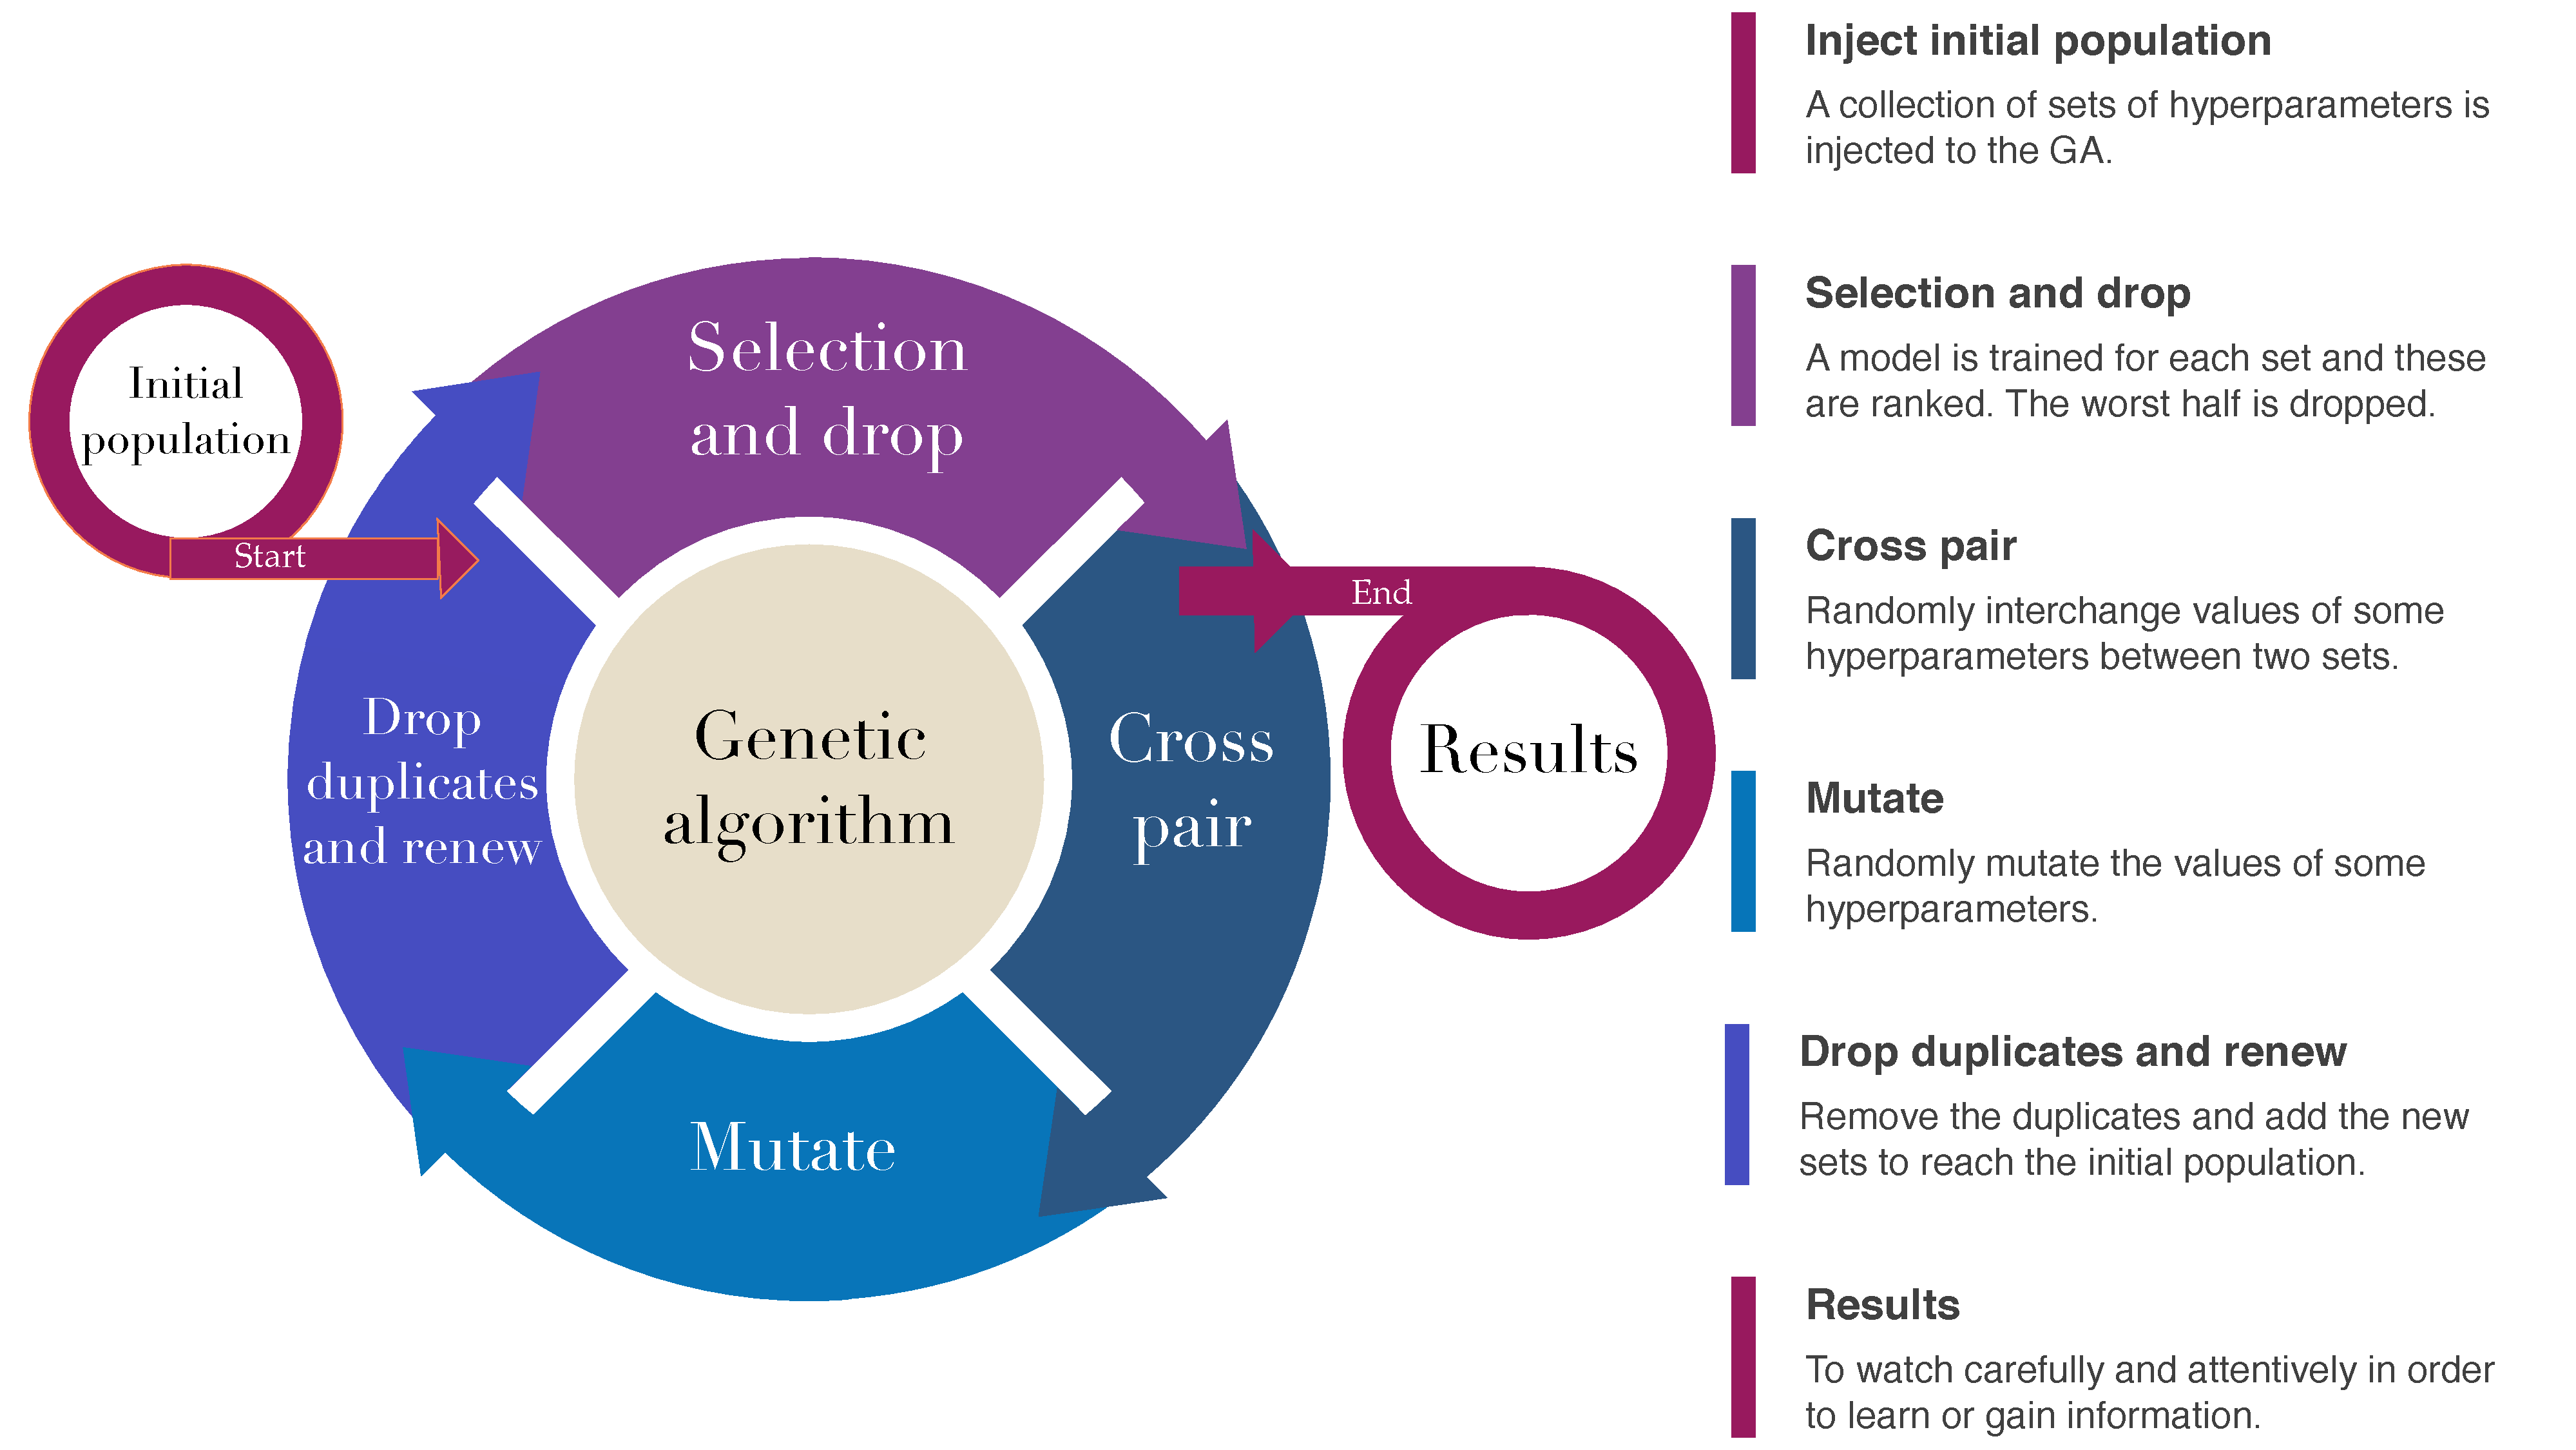
\includegraphics[width=.9\linewidth]{Appendices/BDT/Genetic_Algorithm_Legend_English_NewPalete}
\caption{Schematic view of the GA method for hyperparameter optimisation.}
\label{fig:Appendix:BDT:GA_loop}
\end{figure}



%%%%%%%%%%%%%%
%   Other considerations   %
%%%%%%%%%%%%%%


\section{Other considerations about BDTs}
\label{chap:Appendix:BDT:Concepts}

%\paragraph{Binary splits}\mbox{}\\
%Rather than splitting into two groups at each node, one could consider
%several splits at each stage. Although this has its benefits, it is not a wise 
%general course of action. Multiway splits cause the data to fragment too quickly, 
%leaving the next level below with insufficient data. In the end, binary splits are 
%favoured because they can also be used to create multiclass divides.


% Inestability
%\paragraph{Instability of trees}\mbox{}\\
%The large variance of trees is one of their main issues. A little modification in the 
%data can frequently lead to very different results. This is mainly caused by the
%hierarchical structure of the trees, which causes errors in the top split to cascade 
%down to all splits below it. By attempting to employ a more stable split criterion, 
%this can be somewhat mitigated, but the fundamental instability remains. It is the 
%cost of using the data to infer a straightforward, tree-based structure. 

% ROC
\paragraph{Receiver operating characteristic curve}\mbox{}\\
The receiver operating characteristic curve (ROC) is a graphical plot used
that is used to illustrate the ability of a binary classifier. It assesses the 
tradeoff between true positive (TP) and false negative (FP) rates as the parameters of the classification vary.
This is depicted in Figure~\ref{fig:Appendix:BDT:ROC_AUC:ROC}. 
\begin{itemize}
	\item \textbf{True positive rate}: Also known as sensitivity. 
	It is the possibility of a positive test conditioned on truly being positive. For instance, it is the probability
	for the BDT in Section~\ref{sec:ChaptH:EventSelection:BDT} to identify a \tHq event as such. 
	\item \textbf{False positivity rate}: It can be calculated as 1 - sensitivity. 
	It refers to the possibility of a negative test given that it is truly positive. In the Section~\ref{sec:ChaptH:EventSelection:BDT}
	BDT scenario, it would be the ability to classify a background event as if it was a \tHq signal event.  
\end{itemize}

The area under the curve (AUC) is a commonly used quantitative summary, it measures the
bidimensional area under the ROC from (0,0) to (1,1) as Figure~\ref{fig:Appendix:BDT:ROC_AUC:AUC} shows.
The use of the AUC is convenient for several two reasons. Firstly, it is invariant with the scale because it does
not measure absolute values but rates. Secondly, it is invariant with respect to the classification threshold and,
hence, it evaluates quality of the classification model.

\begin{figure}[h]
\begin{subfigure}[h]{0.45\linewidth}
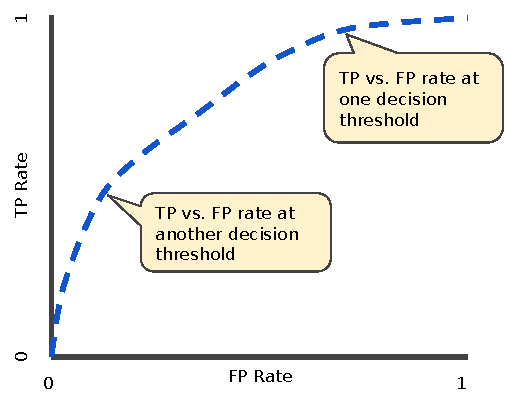
\includegraphics[width=\linewidth]{Appendices/BDT/ROC_AUC_B}
\caption{Typical ROC curve. It shows that as the classification threshold decreases, more events are classified as positive, 
causing both the FP and FN rates to increase.}
\label{fig:Appendix:BDT:ROC_AUC:ROC}
\end{subfigure}
\hfill
\begin{subfigure}[h]{0.45\linewidth}
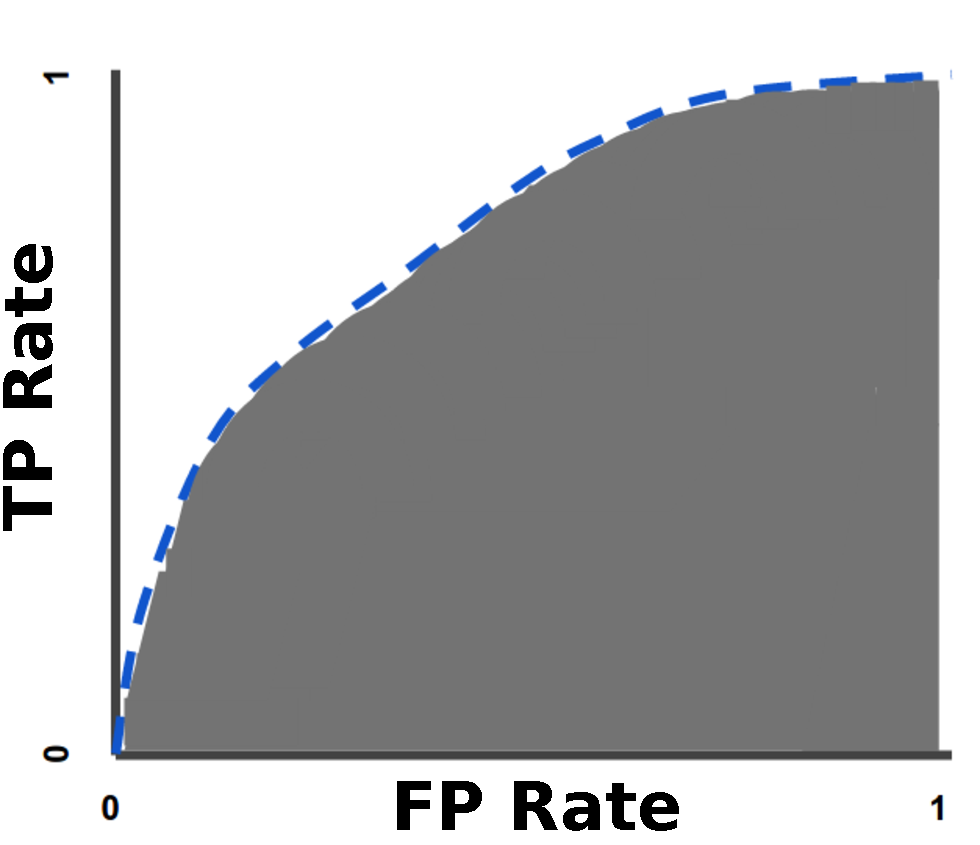
\includegraphics[width=0.8\linewidth]{Appendices/BDT/ROC_AUC_A}
\caption{The AUC varies from 0 to 1. While 0.0 corresponds to a model that always fails, a 1.0 
means that the model is right a 100\% of times.}
\label{fig:Appendix:BDT:ROC_AUC:AUC}
\end{subfigure}%
\caption{The ROC presentes the TP vs the FN rate. The ROC analysis is related
to cost/benefit interpretation of decision making. }
\label{fig:Appendix:BDT:ROC_AUC}
\end{figure}

%\pablo{For the meaning of the different AUC values check the reference: \url{https://www.jto.org/article/S1556-0864(15)30604-3/fulltext} \\ 
%A perfect predictor gives an AUC-ROC score of 1, a predictor which makes random 
%guesses has an AUC-ROC score of 0.5.}

% precision-Recall
\paragraph{Precision-Recall curves}\mbox{}\\
While the ROC summarises the trade-off between 
the true positive rate and false positive rate for a predictive 
for different probability thresholds, there is another plot that helps
with the diagnosis of the binary classification models; the Precision-Recall curves.
These summarise the equilibrium between the true positive rate and 
the positive predictive value for a predictive model using different probability thresholds.

Typically, the use of ROC and precession-recall curves is such that the first type is used
when there are roughly equal numbers of observations for each class and
the second should be used when there is a moderate to large class imbalance.
%% Justo al revés de como lo hacemos xD

\begin{figure}[h]
\centering
  \centering
  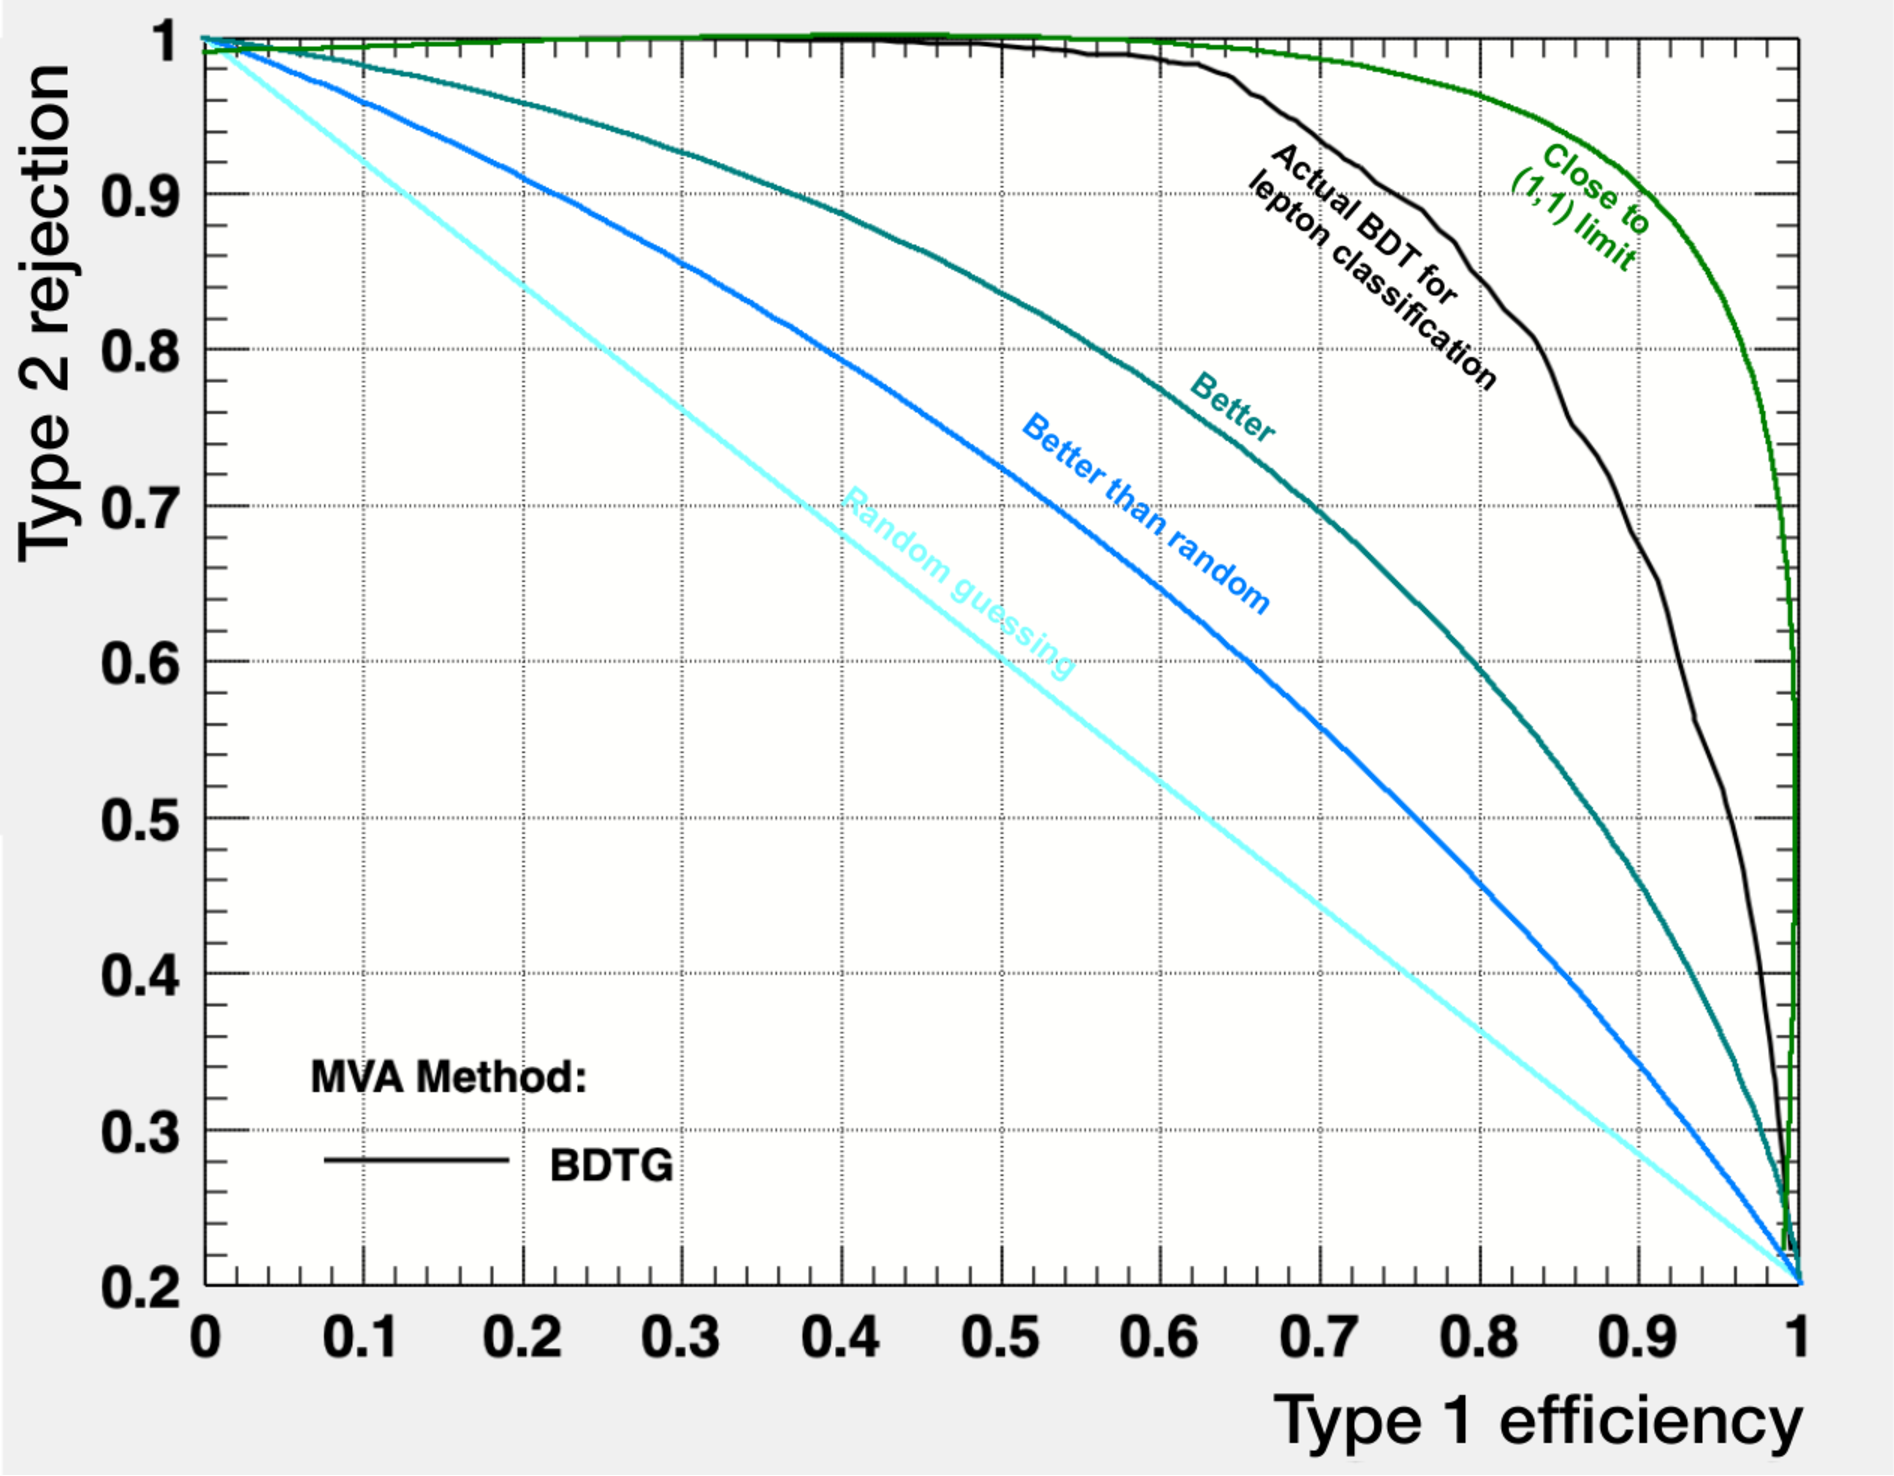
\includegraphics[width=.64\linewidth]{Appendices/BDT/precision-recall_pdf}
\caption{Precision-recall curves for different models. The one in black corresponds to the
$\text{BDT}^{\text{Lepton Assignment}}$ model. The larger is the area under the curve,
the better is the model.}
\label{fig:Appendix:BDT:precision-recallCurve}
\end{figure}

For both the ROC and the precision-recall curves, the larger the area under the curve, the better.
Figure~\ref{fig:Appendix:BDT:precision-recallCurve} shows that the optimal classifier is the one in 
which the curve in the precision-recall plot is close to the (1,1) point.


% KS test
%\paragraph{Kolmogorov-Smirnov test}\mbox{}\\
%In statistics, the Kolmogorov-Smirnov (KS) test is a non-parametric method for comparing the equality 
%of one-dimensional probability distributions. It is used to assess the similarity between 
%a sample distribution and a reference probability distribution.

%In the context of multivariate analysis, 
%the distributions tested by the KS are the scores of the test and train. In other words, 
%the test sample. If the score is close to zero, it may imply that the classifier is overtrained.
%In the way it is implemented in TMVA, the ideal value is 0.5, although being above 0.01 is
%considered enough.

%For any two random samples drawn from the same parent distibution, the
%KS test value would be distributed uniformly between 0 and 1. So ..
%so if you training weren't biased at all towards the training
%sample (note: this bias does not necessarily represent overtraining)
%then you'd for you test / training sample 'on average' expect a KS
%value of 0.5

%Some sources argue that KS test requires a large sample to be effective.
%This  may explain the low values in for all folds in the TMVA gradient
%BDT used for the lepton-origin assignment.
% Source about sample size: https://root-forum.cern.ch/t/overtraining-test-obtained-from-tmva/32148
% Discussion; https://root-forum.cern.ch/t/kolmogorov-smirnov-test-values/32868

 
% Separation power
\paragraph{Separation power}\mbox{}\\
The separation power is a valuable metric for evaluating the performance 
of a variable or classifier in terms of its ability to distinguish the target process 
from other processes. The separation power $<S^{2}>$ of a classifier $y$ can 
be quantified using the integral:
\begin{equation}\label{eq:Appendix:BDT:SeparationPower}
	<S^{2}> = \frac{1}{2}\int \frac{(\hat{y}_{S} - \hat{y}_{B})^{2}}{\hat{y}_{S}+\hat{y}_{B}}dy \, ,
\end{equation}
where $\hat{y}_{S}$ and $\hat{y}_{B}$ are, respectively, the signal and background probability 
density functions of $y$.  The 1/2 factor is used to keep $<S^{2}>$ within the [$0, 1$] interval.
The separation is zero for identical signal and background shapes, and 
it is one for shapes with no overlap.



%%%%%%%%%%%%%%%%%%%%%
%             Extra plots and tables            %
%%%%%%%%%%%%%%%%%%%%%
\section{Additional plots and tables}
\label{sec:BDT:AdditionalMaterial}
This section expands the information provided in the main body of the thesis 
about the training of the different BDT models. The models and ROC curves
of the $\text{BDT}^{\text{Lepton Assignment}}$ are presented in the first
section. The second section shows, for
the XGBoost.based BDT, the correlation between the variables and the evolution of the training.

%%%%%%% Extra plots ::   Assignment
\subsection{$\text{BDT}^{\text{Lepton Assignment}}$}
\label{sec:BDT:AdditionalMaterial:Assignment}
Figure~\ref{fig:dileptau:Assignment_appendix:ScoreDistributions} compare the train and test
distributions for the five different models composing the final $\text{BDT}^{\text{Lepton Assignment}}$.
A good agreement between the distributions of the train and test subsets is observed through all
the folds. This means that no overtraining in our data.
See Section~\ref{sec:ChaptH:Sig:LepAsign:SS:BDT:Training} for the description
of the training of these models.

\begin{figure}[h]
\centering
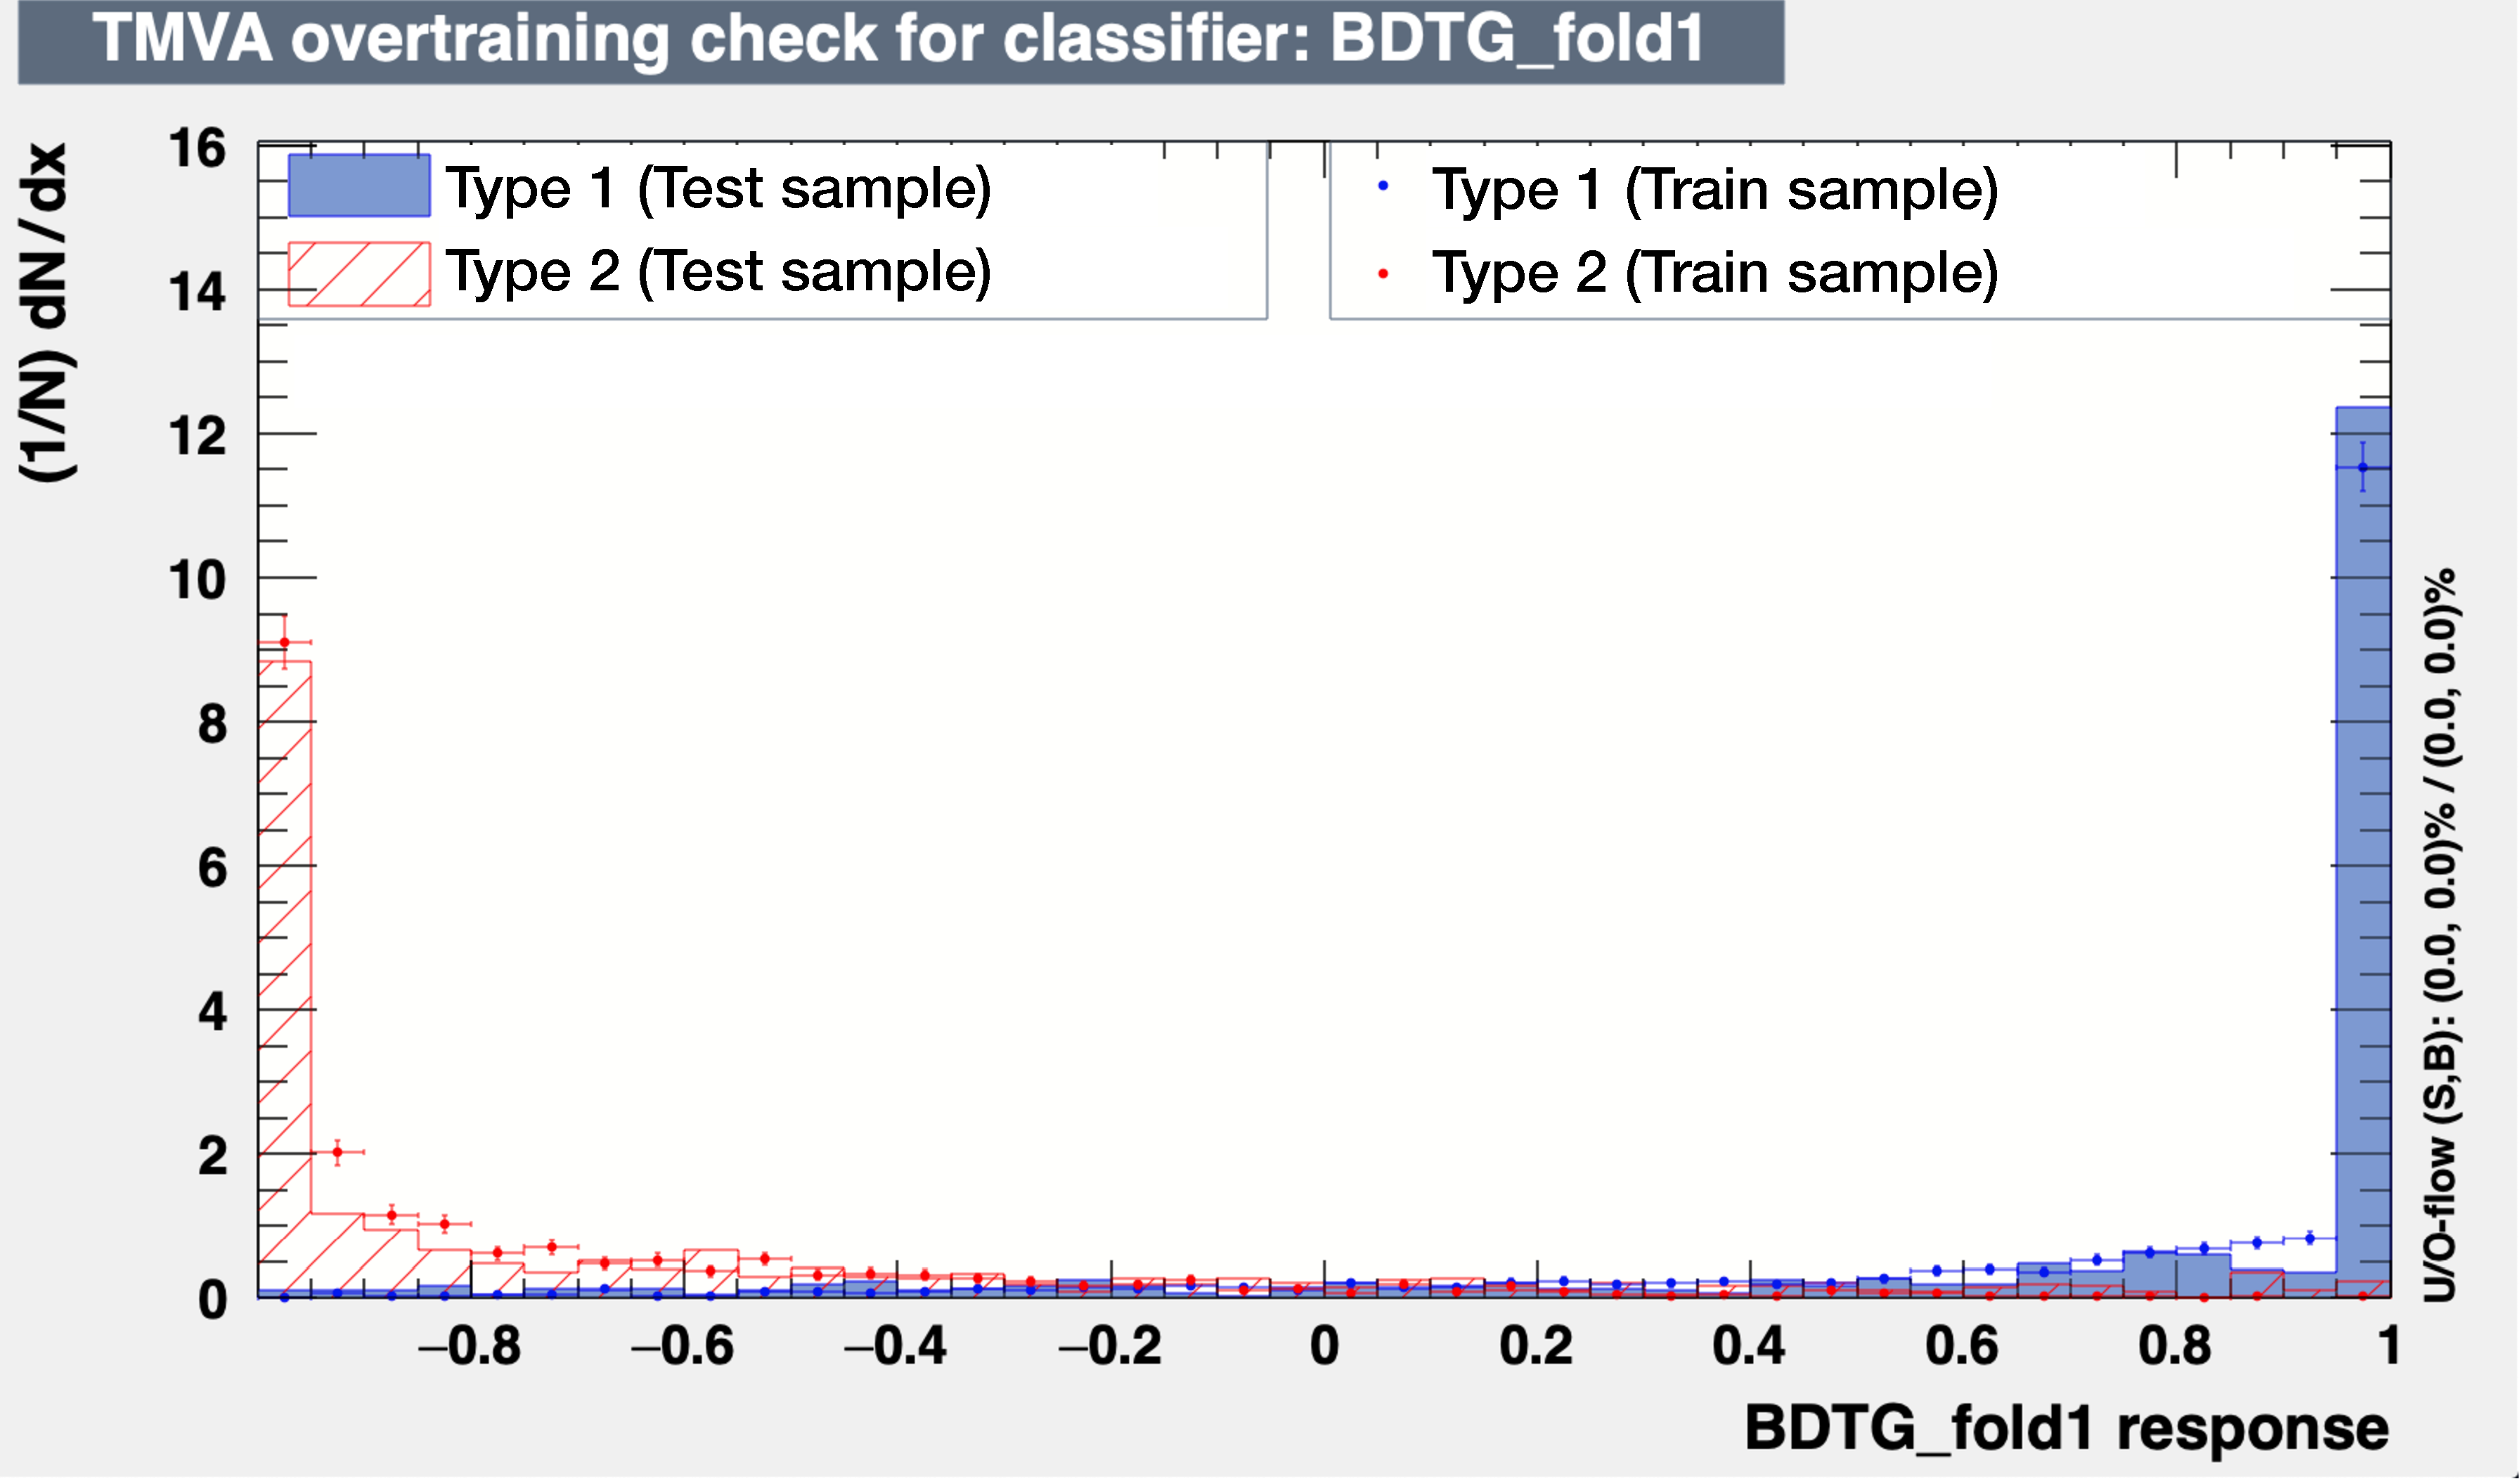
\includegraphics[width=.45\textwidth]{Chapter5_tHq/LeptAssociation/Dileptau_BDT_Based_Assignment_Score_Fold1}\quad
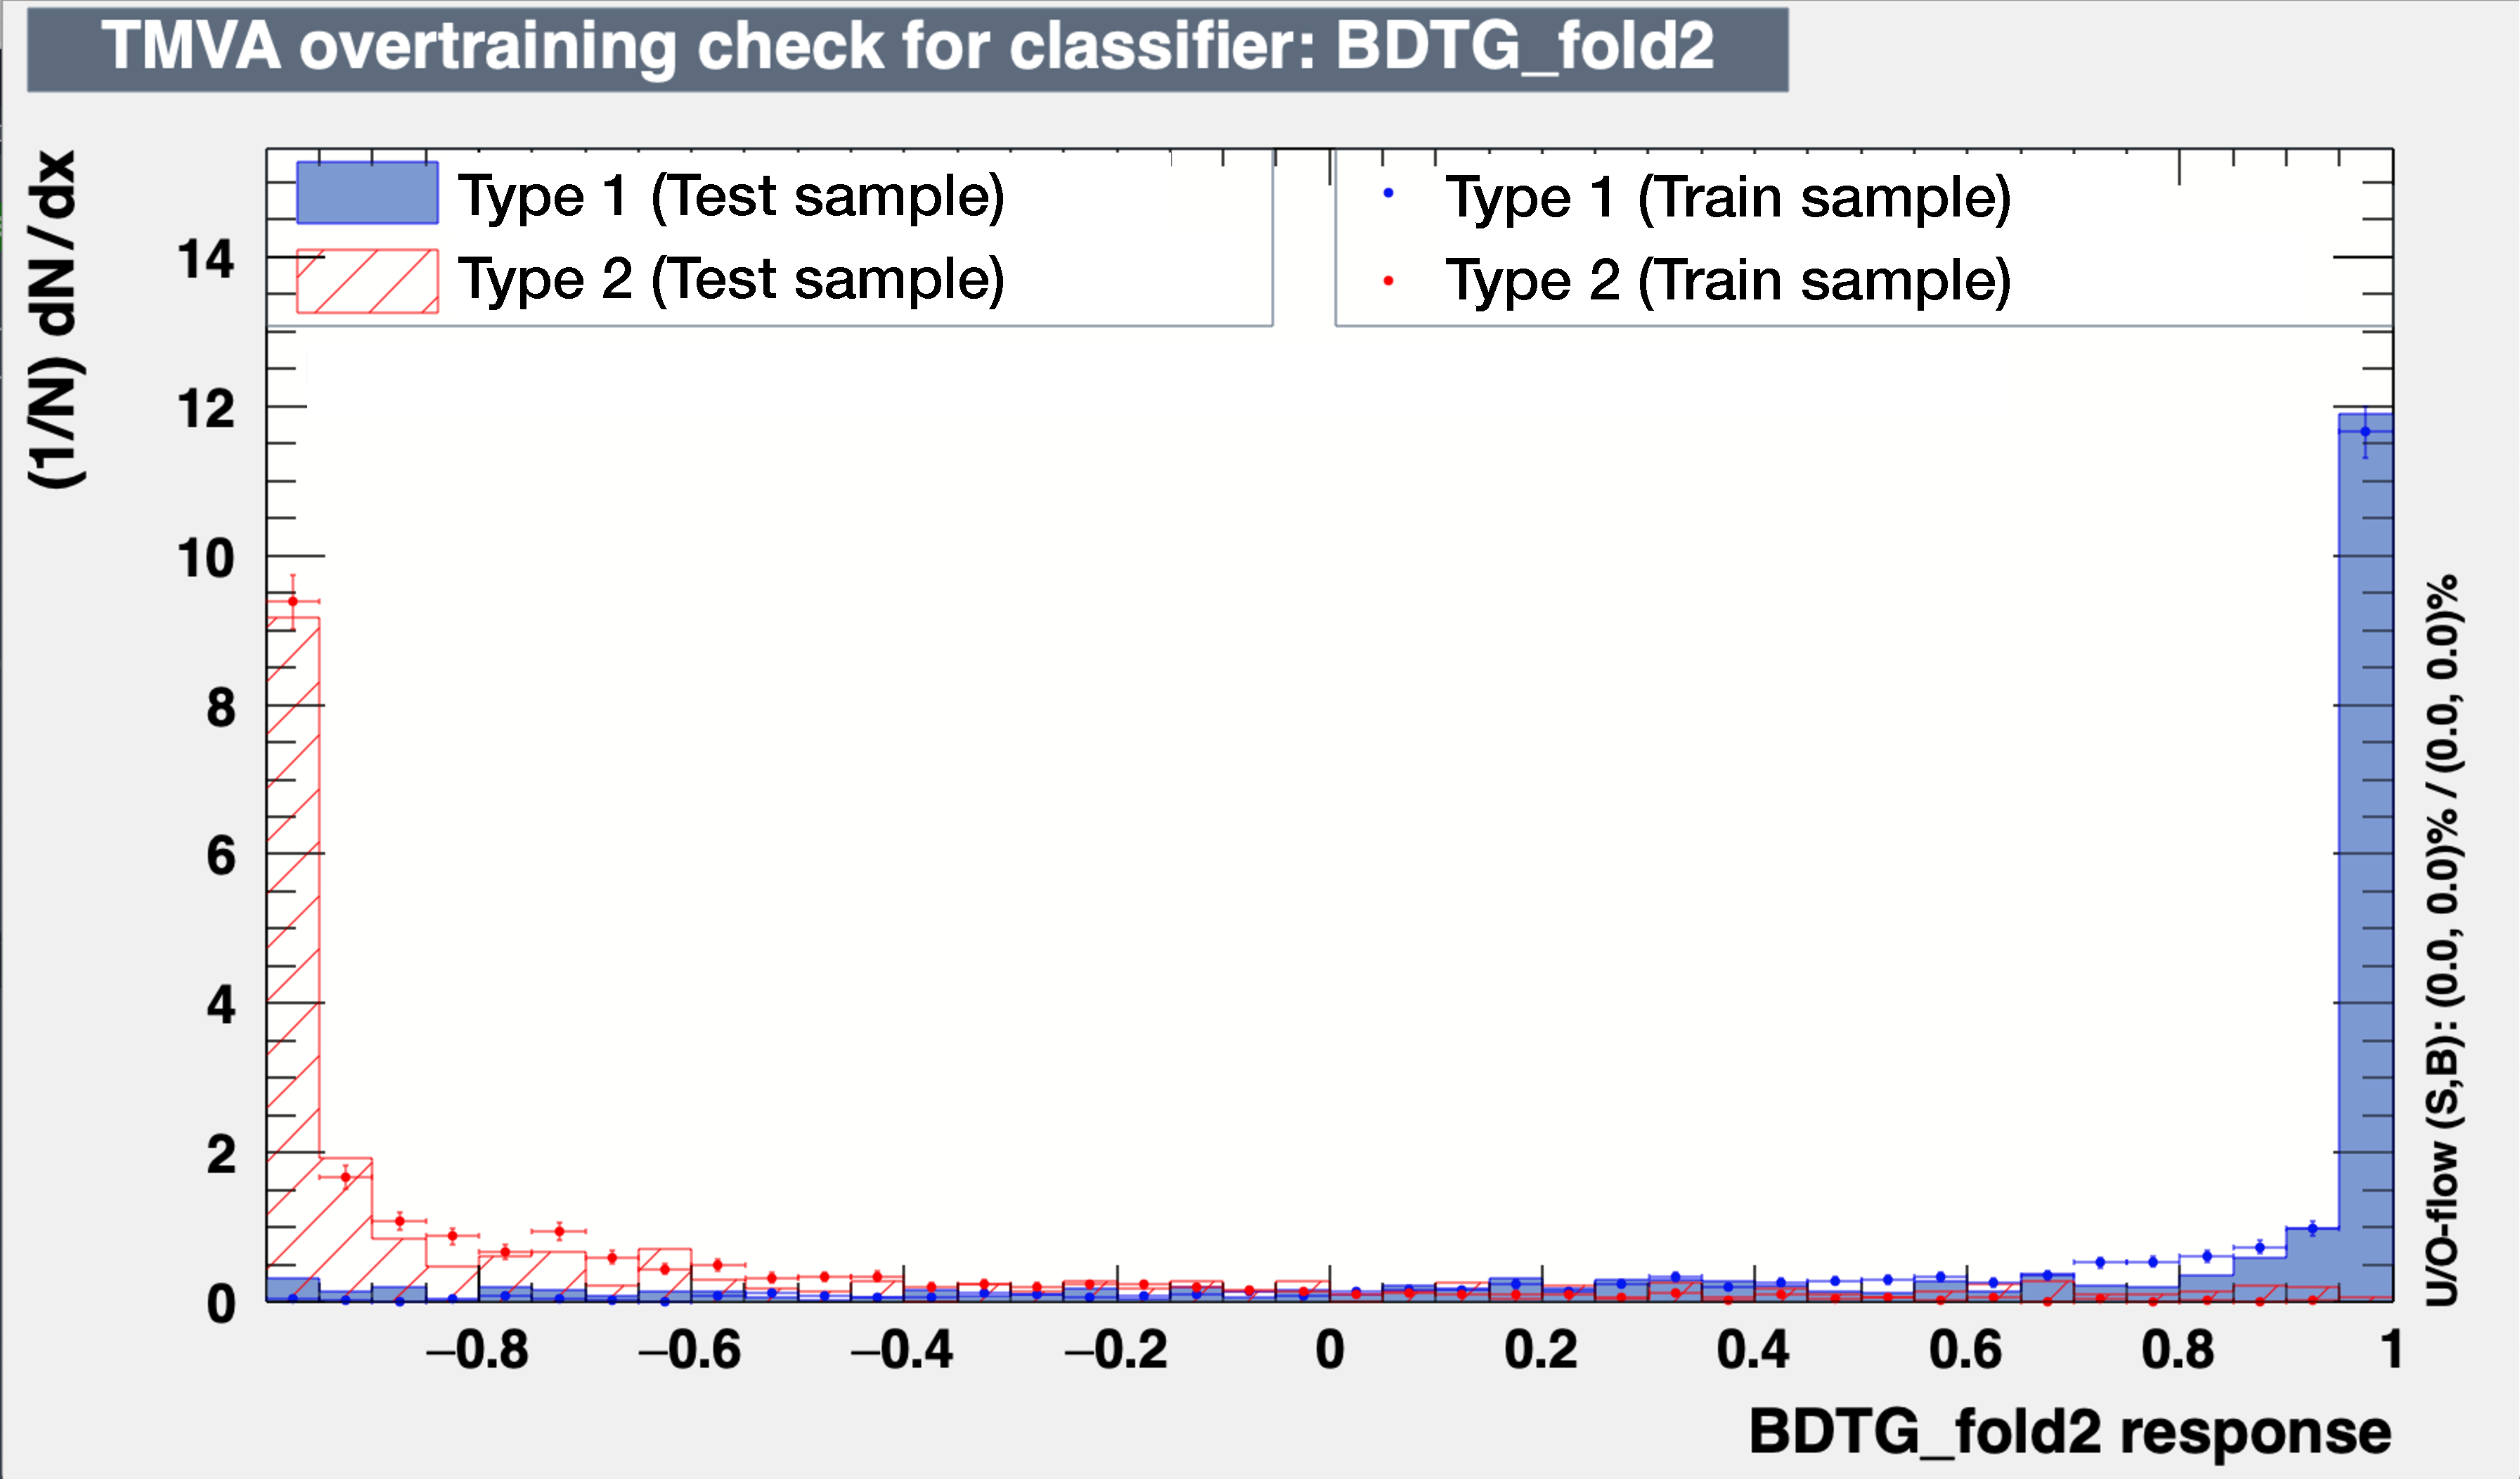
\includegraphics[width=.45\textwidth]{Chapter5_tHq/LeptAssociation/Dileptau_BDT_Based_Assignment_Score_Fold2}
\medskip
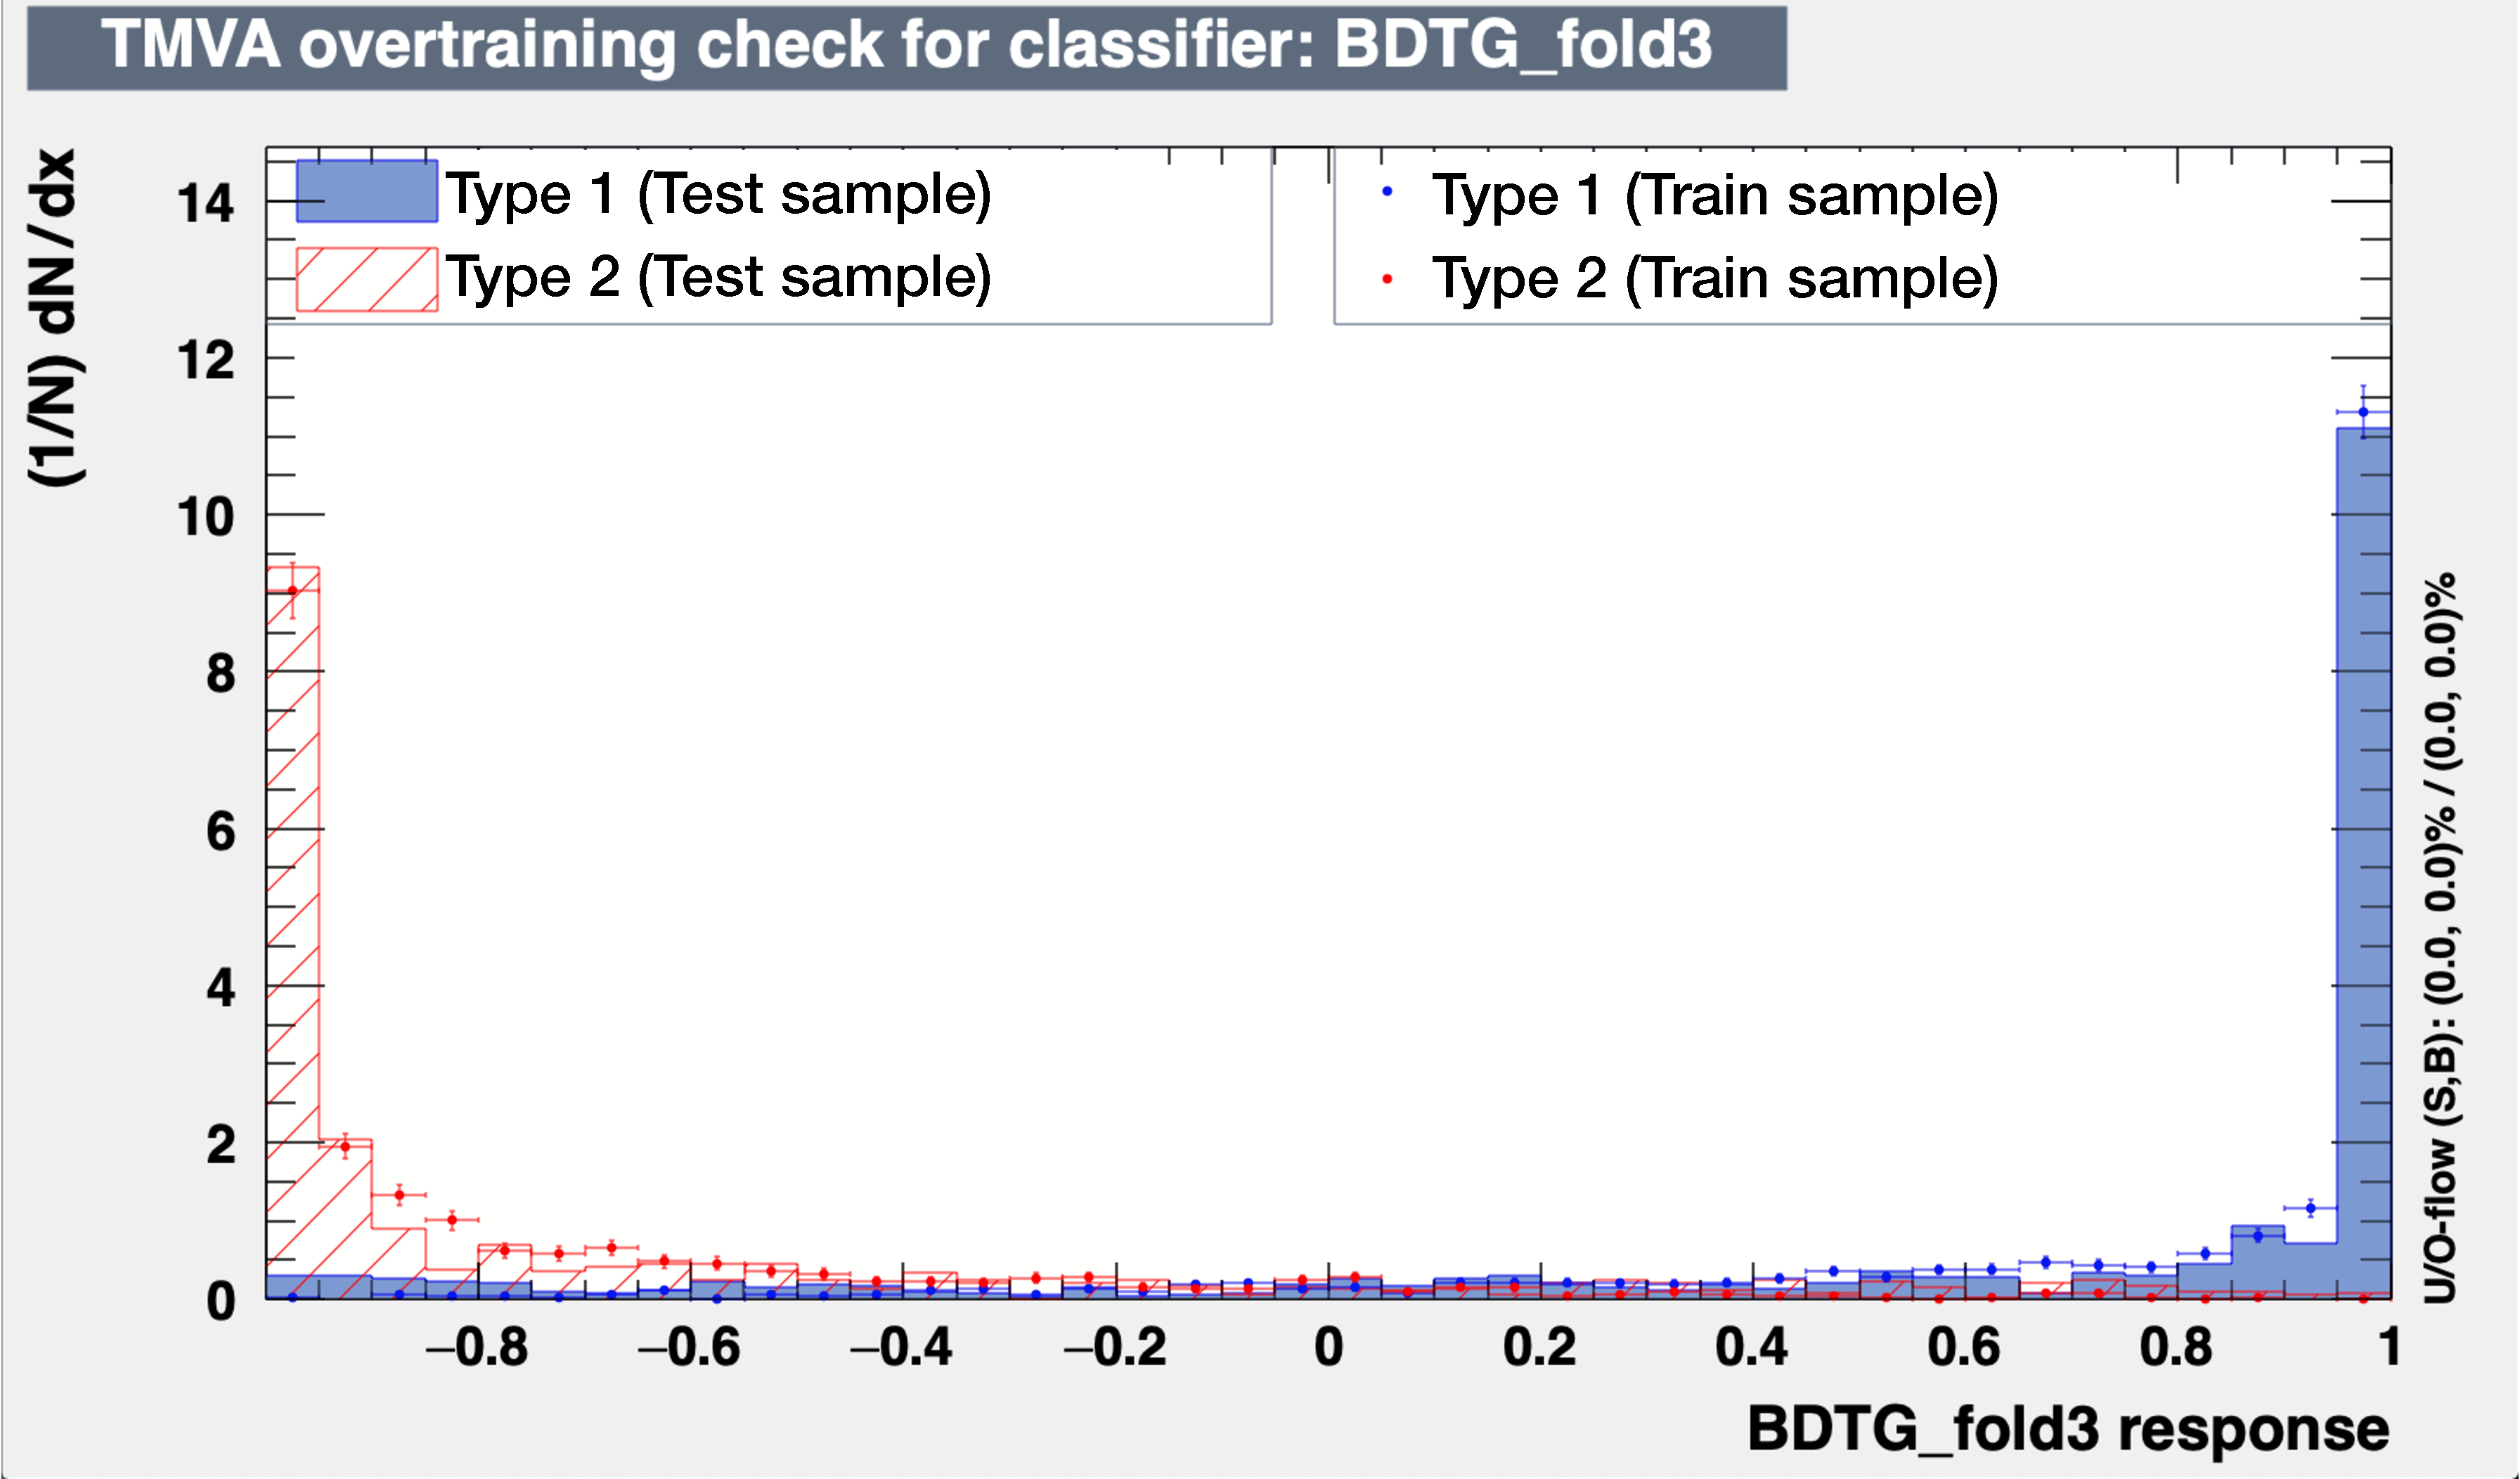
\includegraphics[width=.45\textwidth]{Chapter5_tHq/LeptAssociation/Dileptau_BDT_Based_Assignment_Score_Fold3}\quad

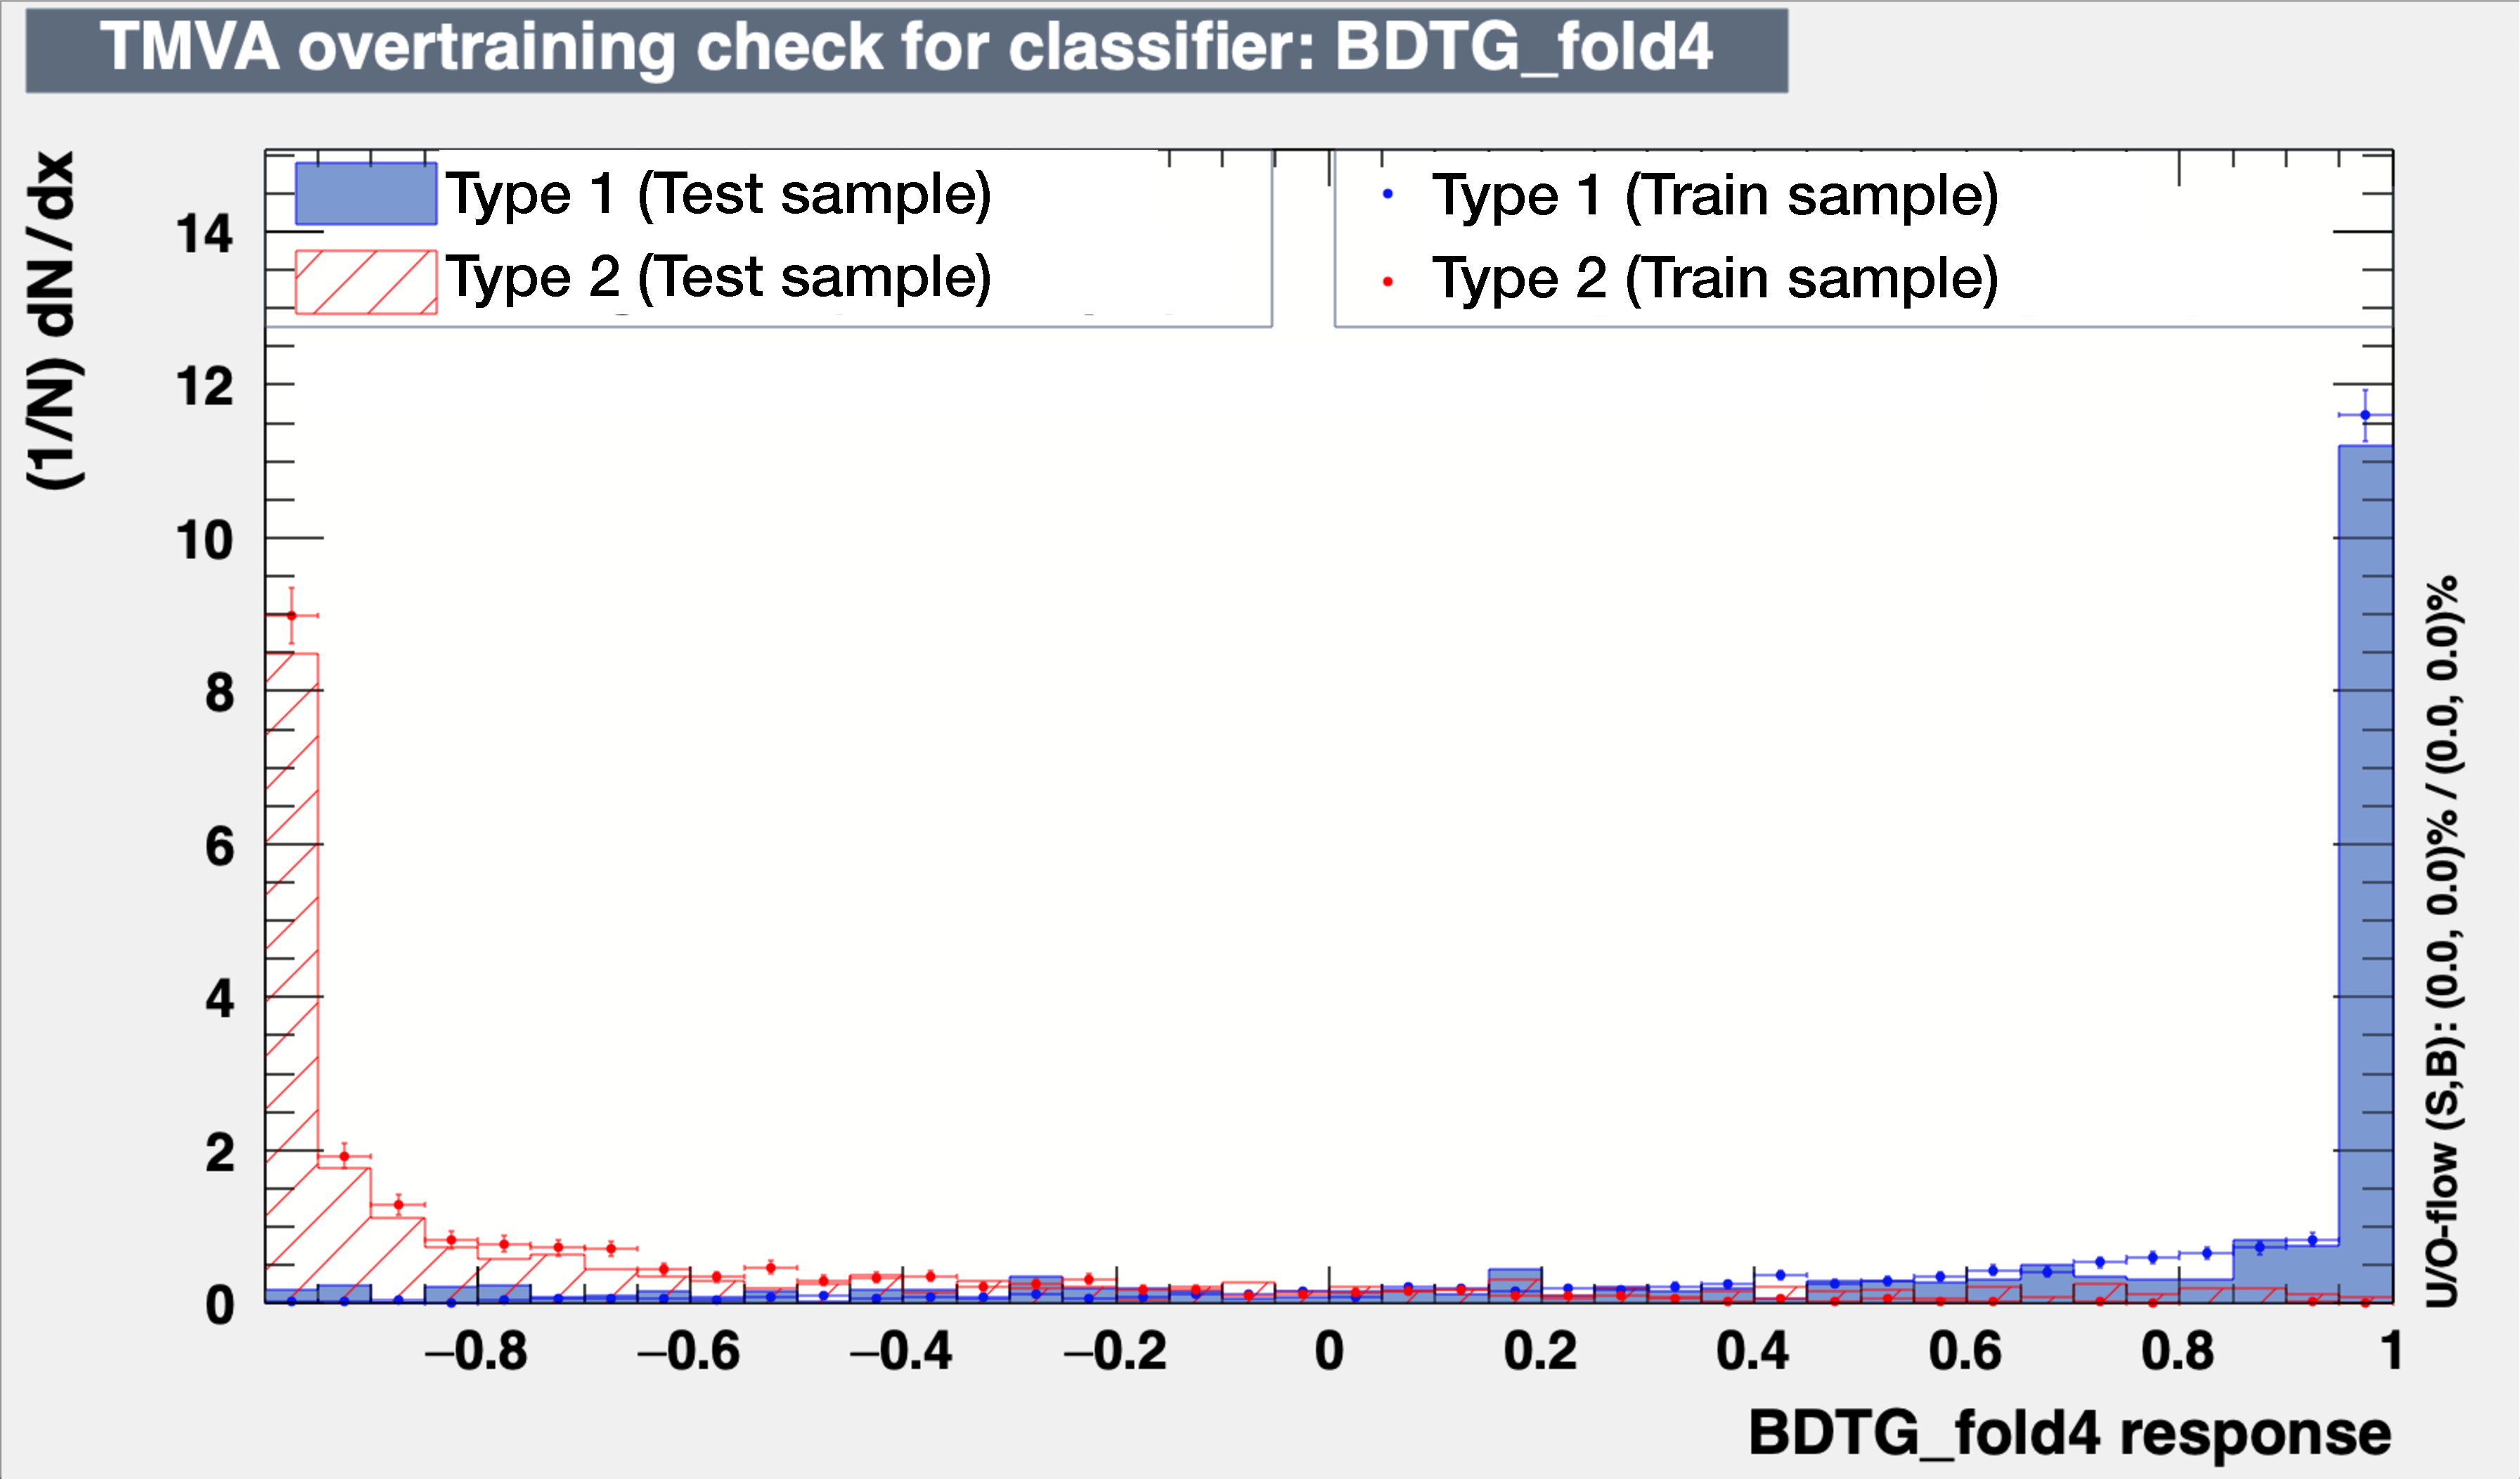
\includegraphics[width=.45\textwidth]{Chapter5_tHq/LeptAssociation//Dileptau_BDT_Based_Assignment_Score_Fold4}
\medskip
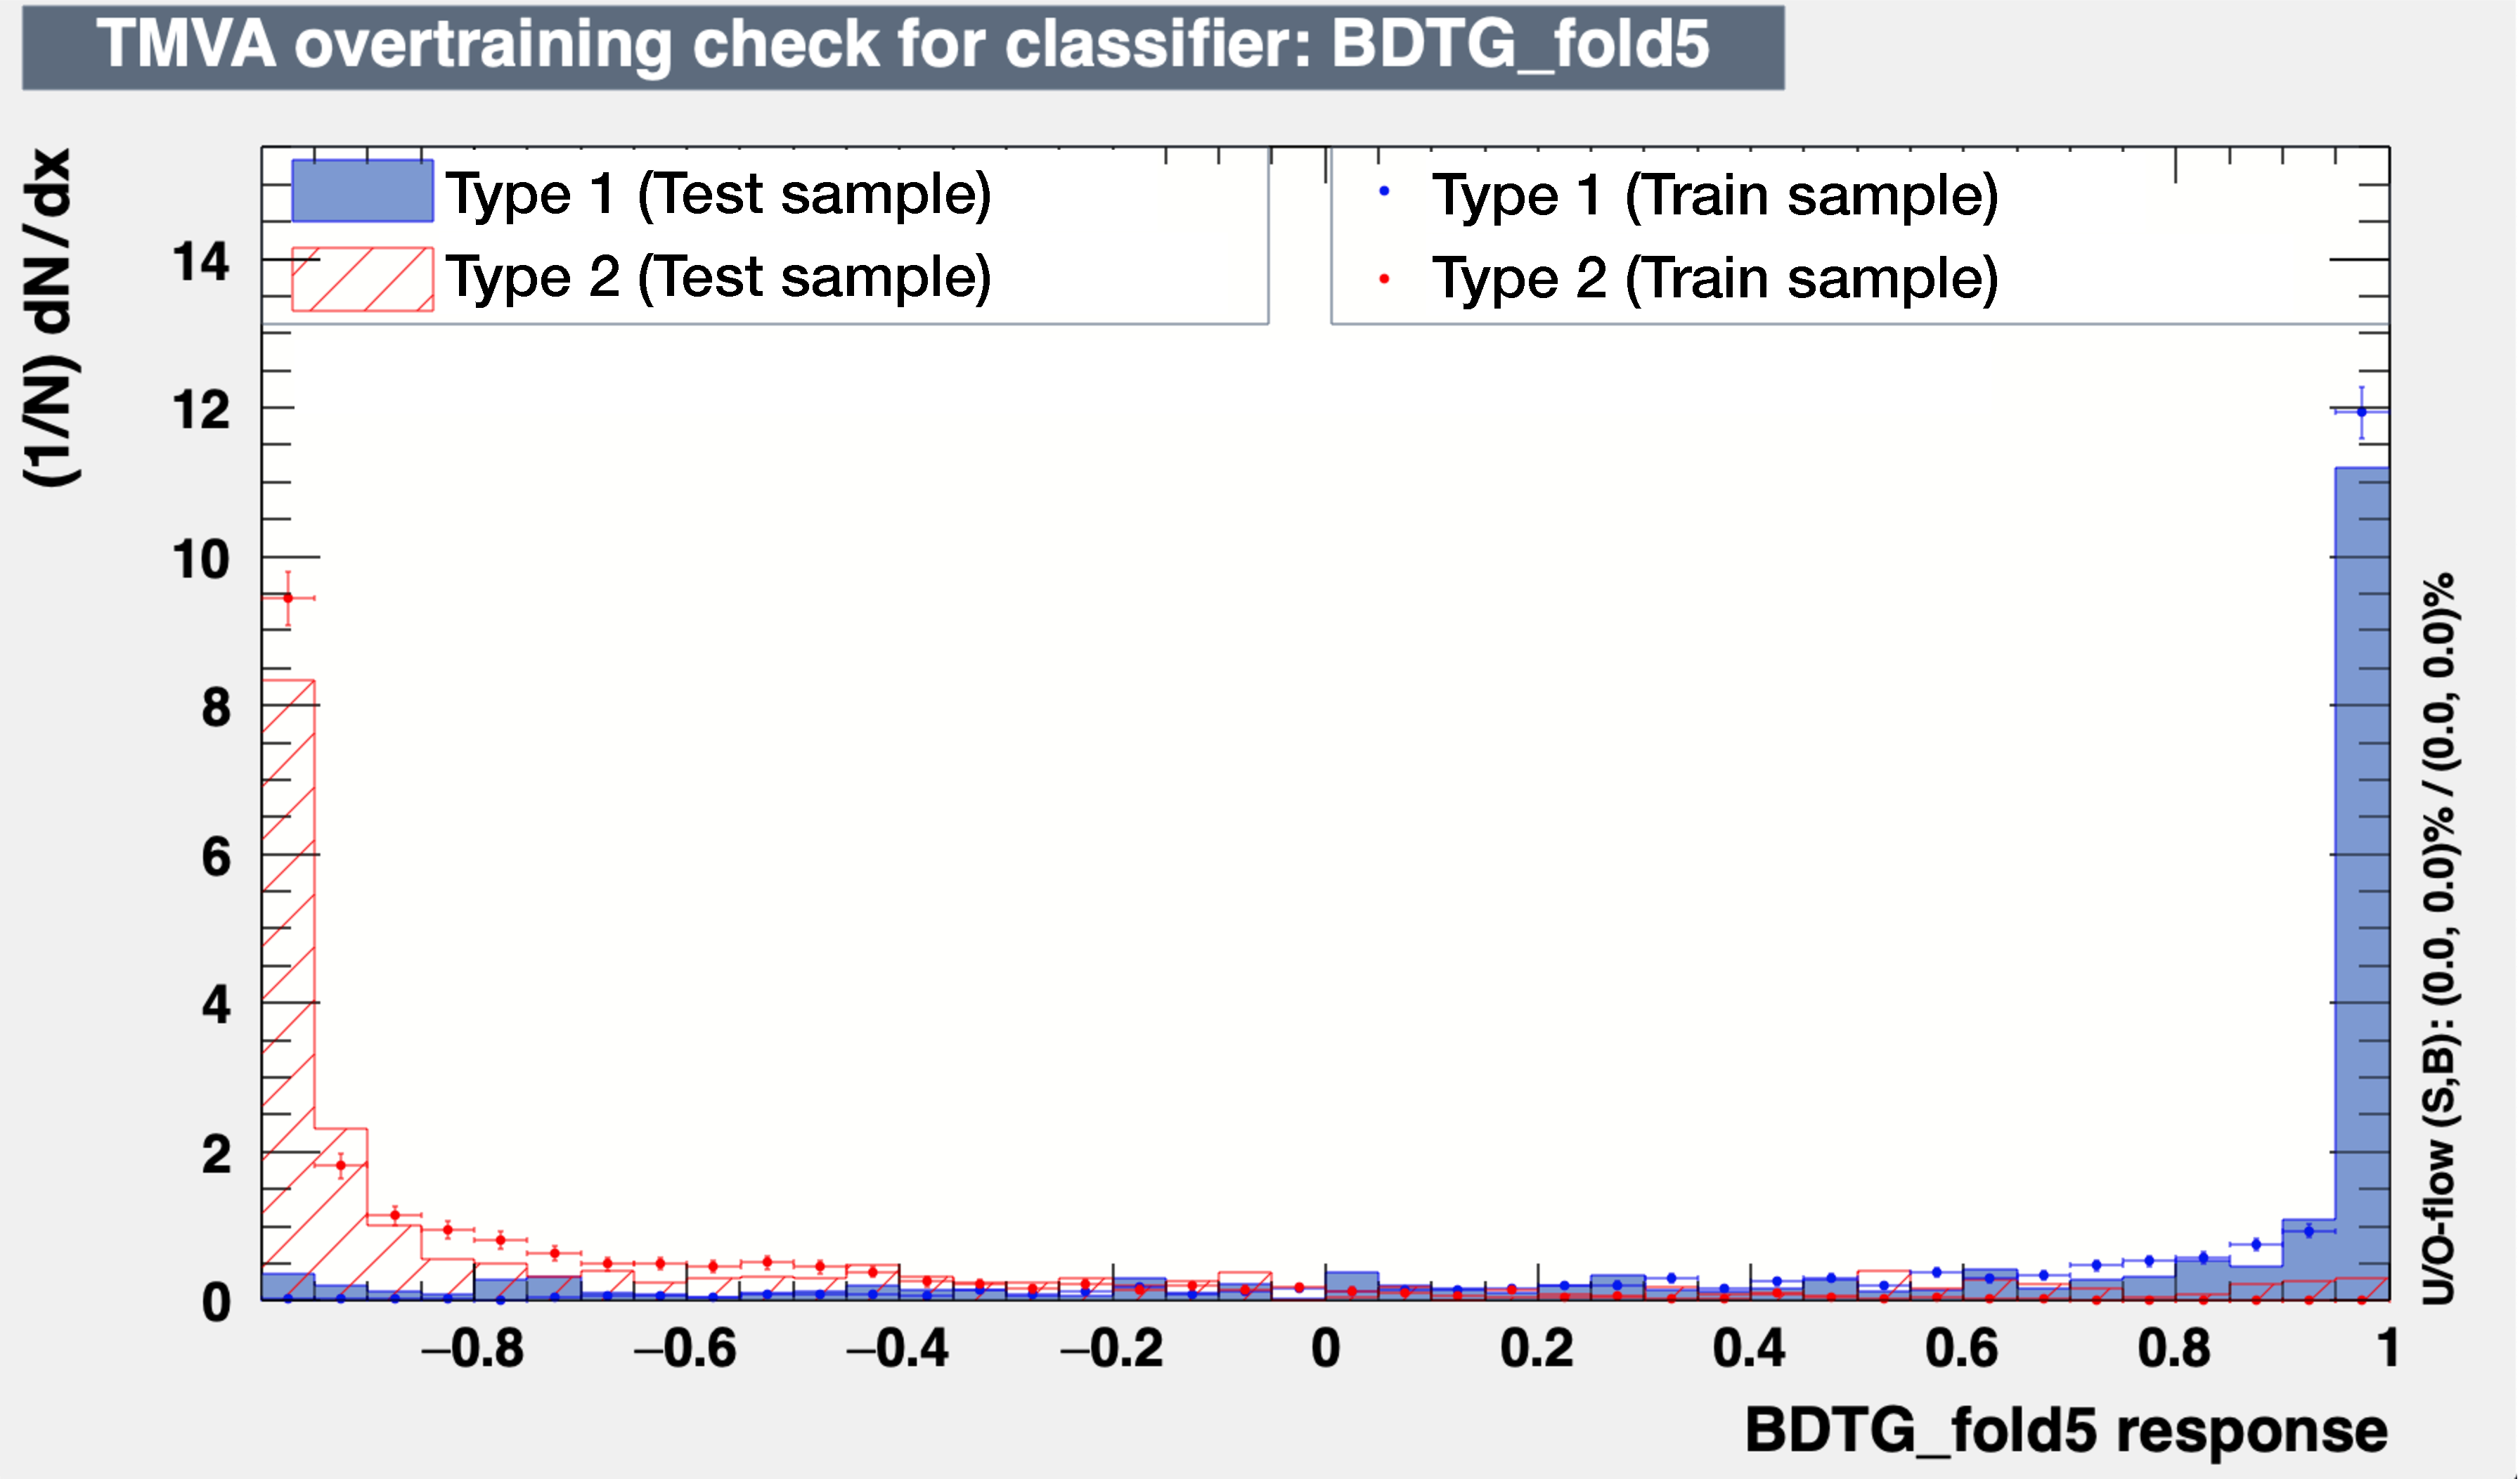
\includegraphics[width=.45\textwidth]{Chapter5_tHq/LeptAssociation/Dileptau_BDT_Based_Assignment_Score_Fold5}
\caption{$\text{BDT}^{\text{Lepton Assignment}}$ distributions for the different folds.
 Type$\,$1 and Type$\,$2 categories are presented in blue and red, respectively.
The doted distribution corresponds to the scores when the model is evaluated on the
training sample. The areas on the histogram refer to the score of the same model when
applied to the test sample. 
%The train and test samples  are superimposed, allowing to check for overtraining. 
On one side, these plots allow to compare the model of each fold. As can be seen,
both categories have the same behaviour through the five models. This indicates
that the subset of the MC sample used in each split is not affecting the model.
On the other side, it can also be checked that the distribution for each fold
is the same for the train and the test subsamples.}
\label{fig:dileptau:Assignment_appendix:ScoreDistributions}
\end{figure}

In Figure~\ref{fig:dileptau:Assignment_appendix:ROCs} are presented the ROC curves for the five models
trained in Section~\ref{sec:ChaptH:Sig:LepAsign:SS:BDT:Training}
 

\begin{figure}[h]
\centering
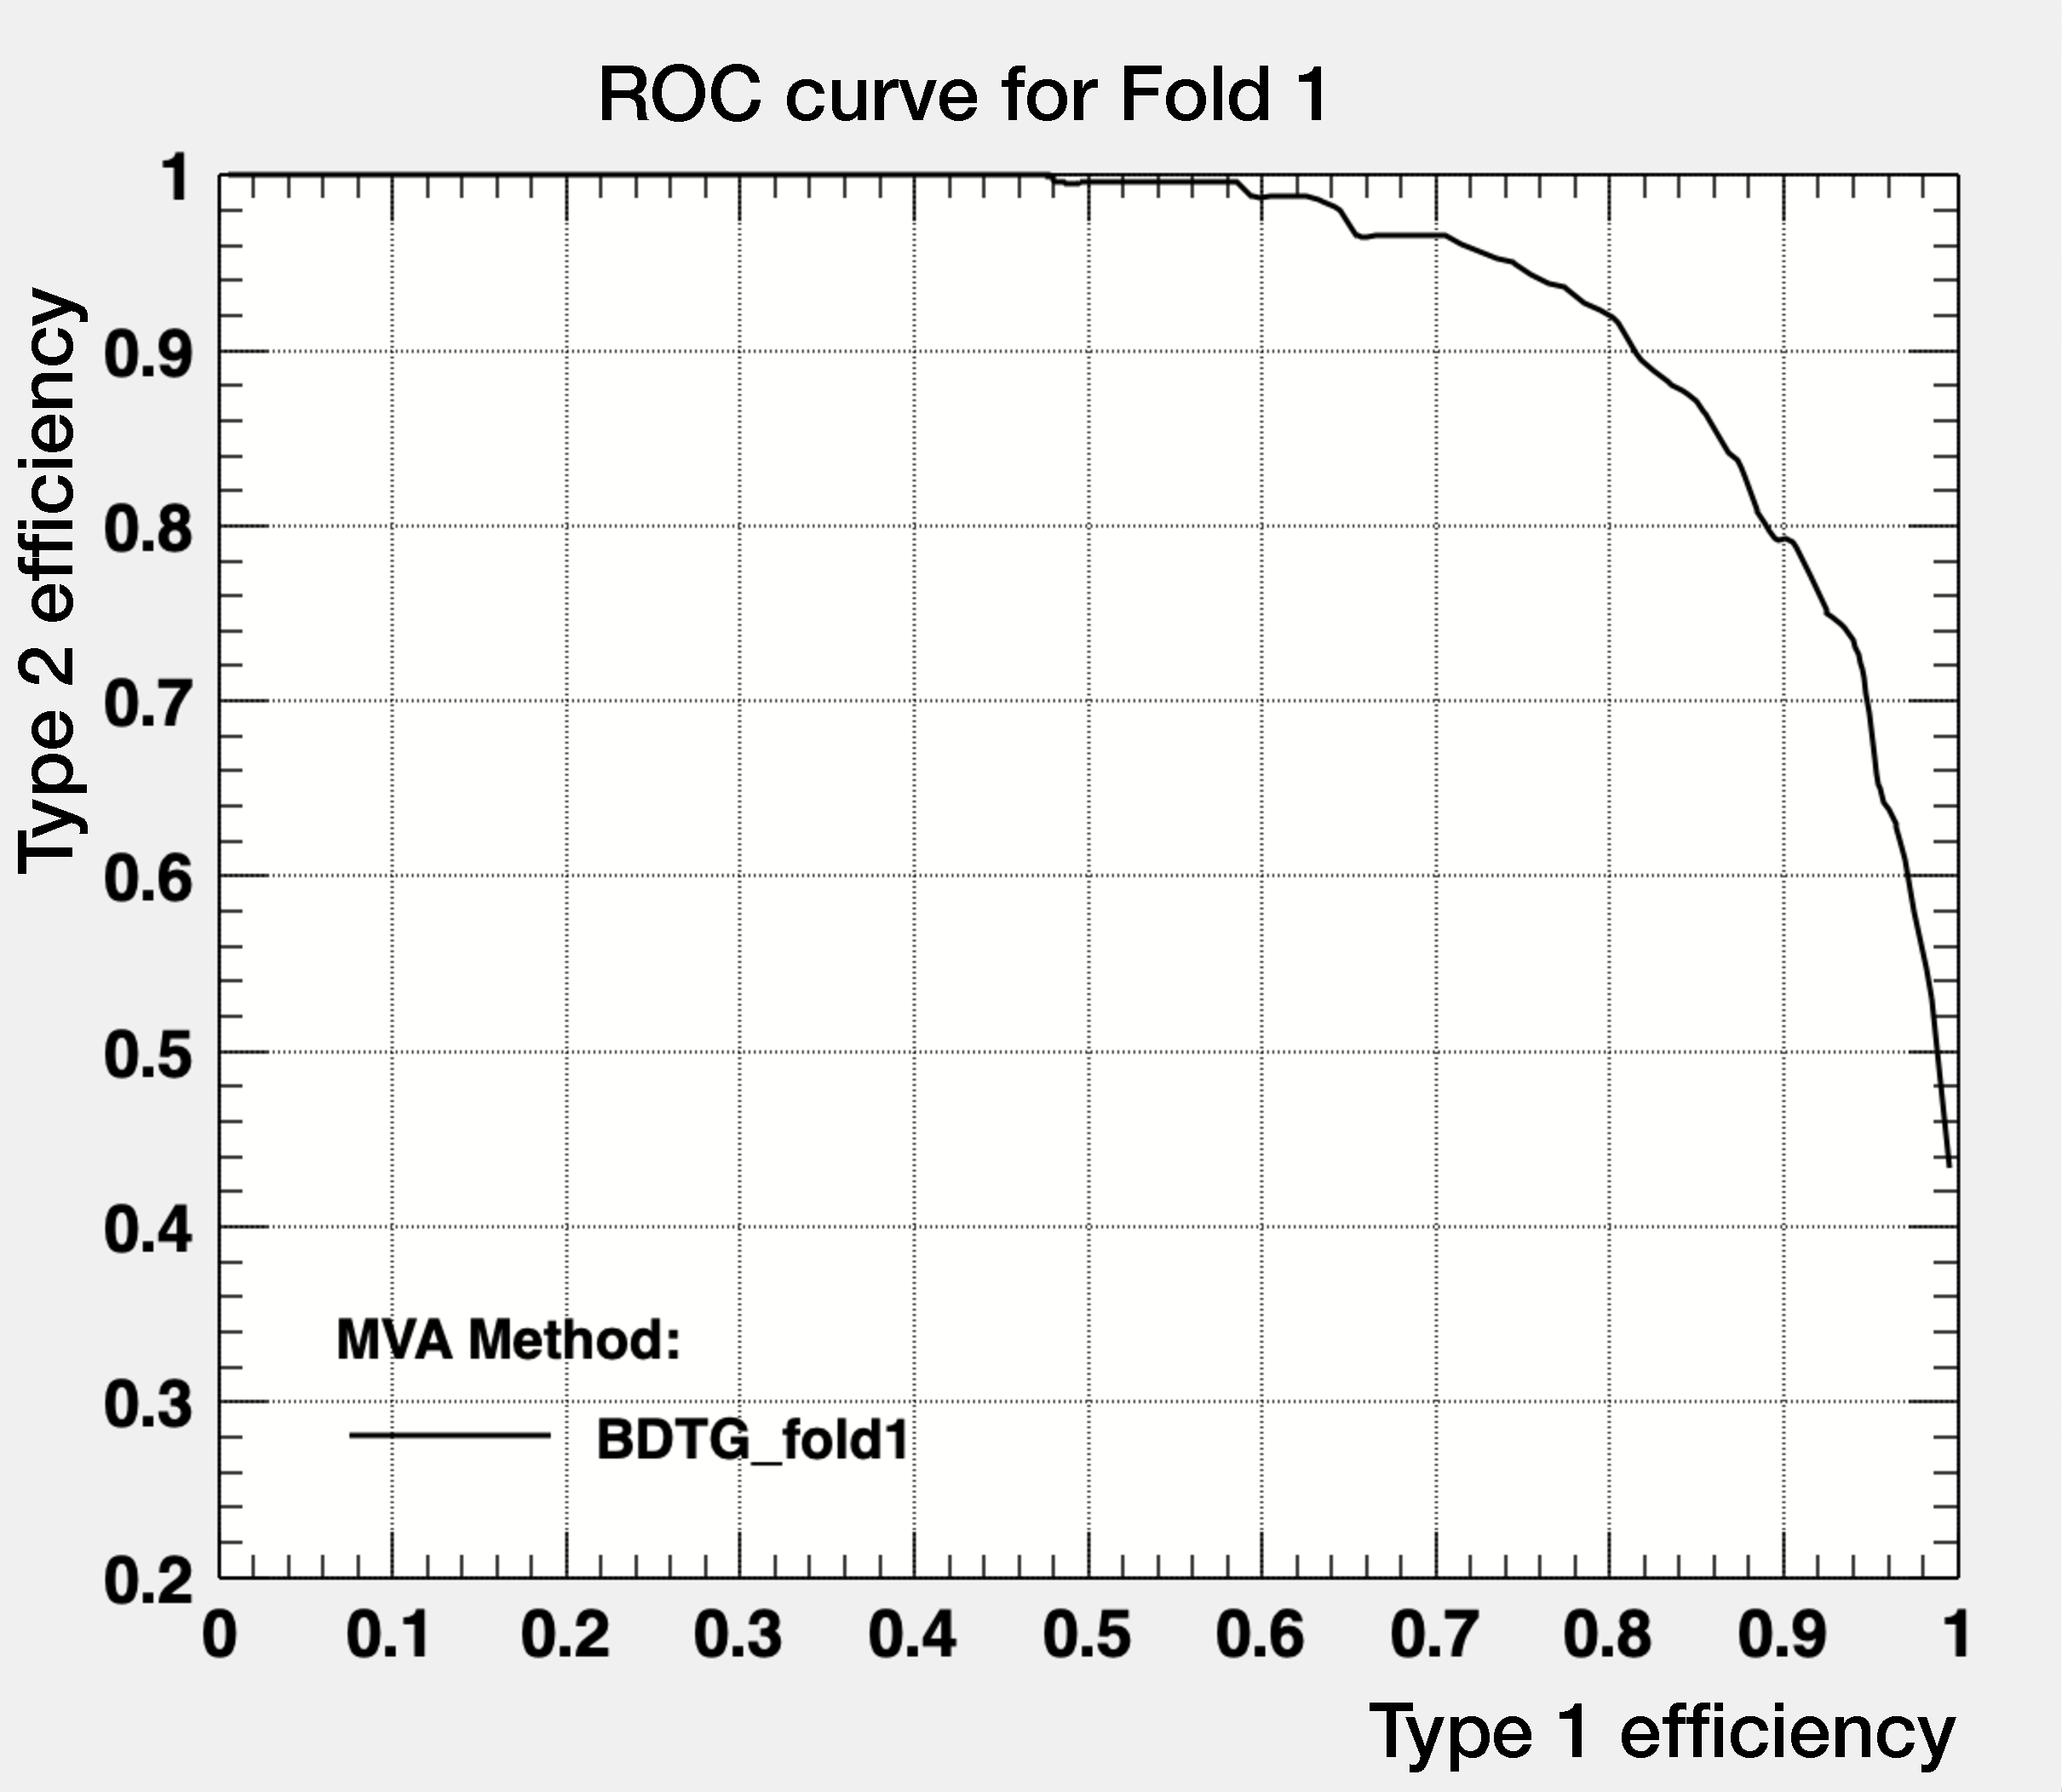
\includegraphics[width=.3\textwidth]{Chapter5_tHq/LeptAssociation/dileptau_ROC_Curve_Fold1}\quad
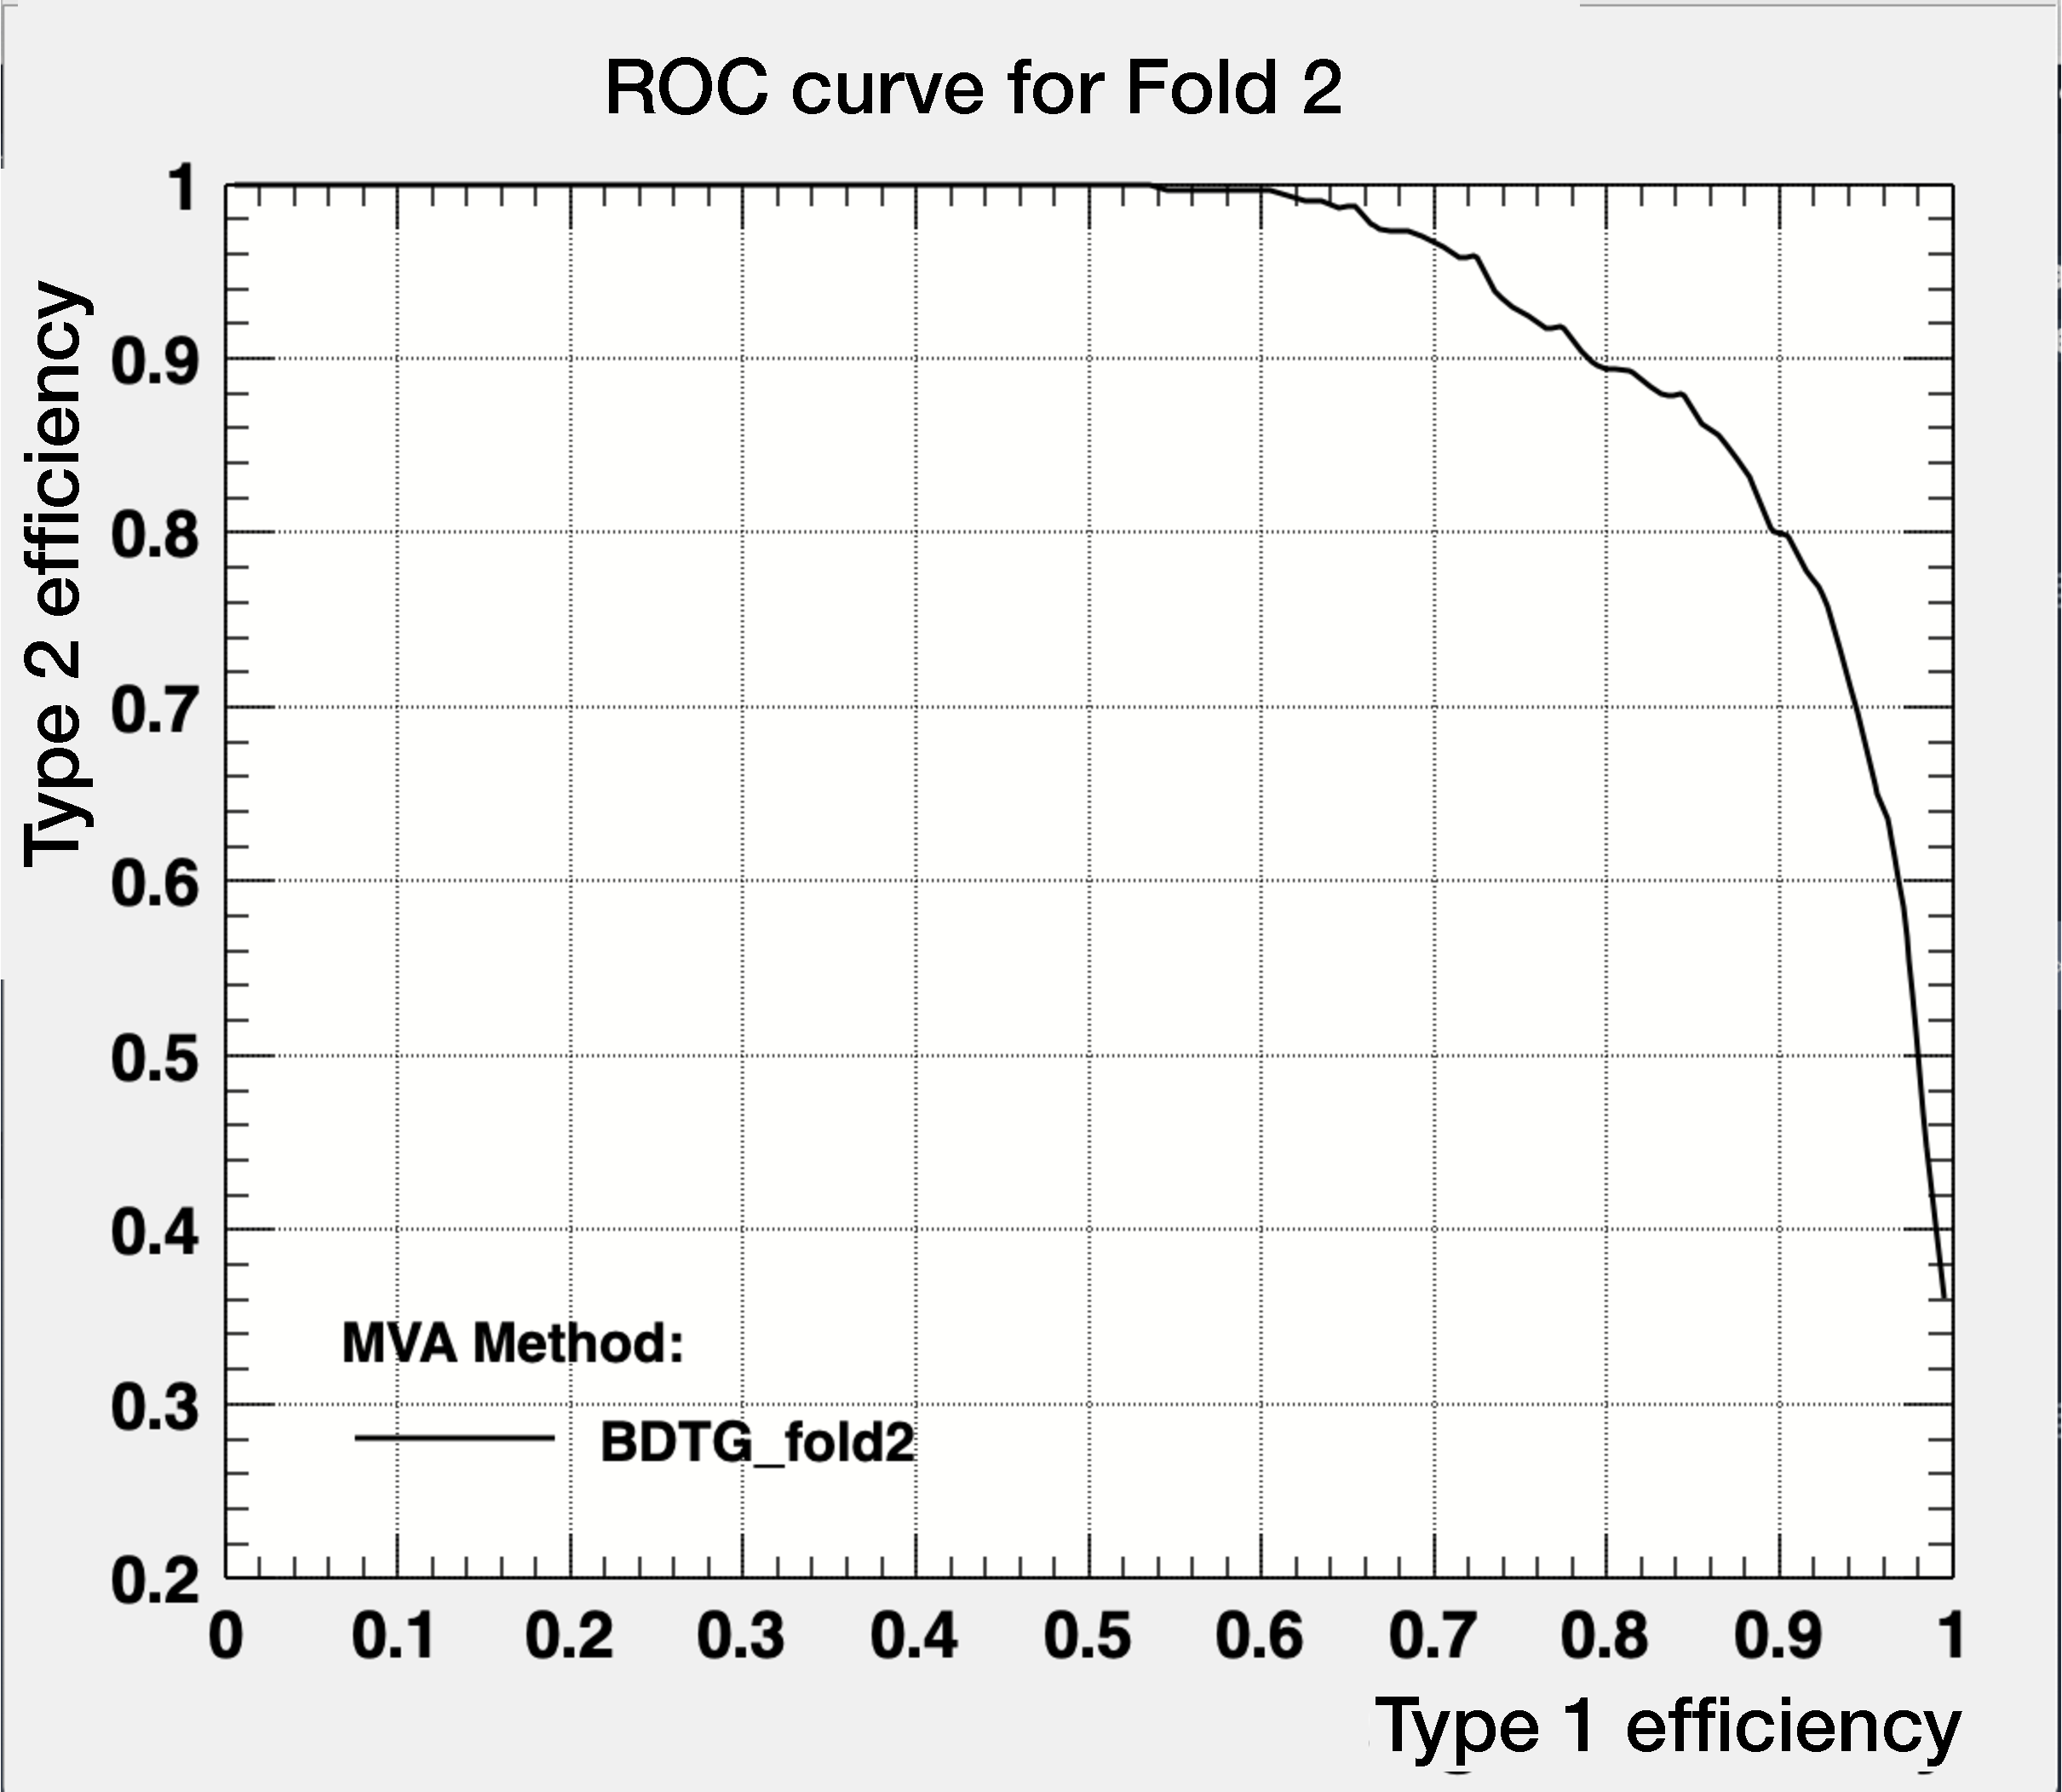
\includegraphics[width=.3\textwidth]{Chapter5_tHq/LeptAssociation/dileptau_ROC_Curve_Fold2}\quad
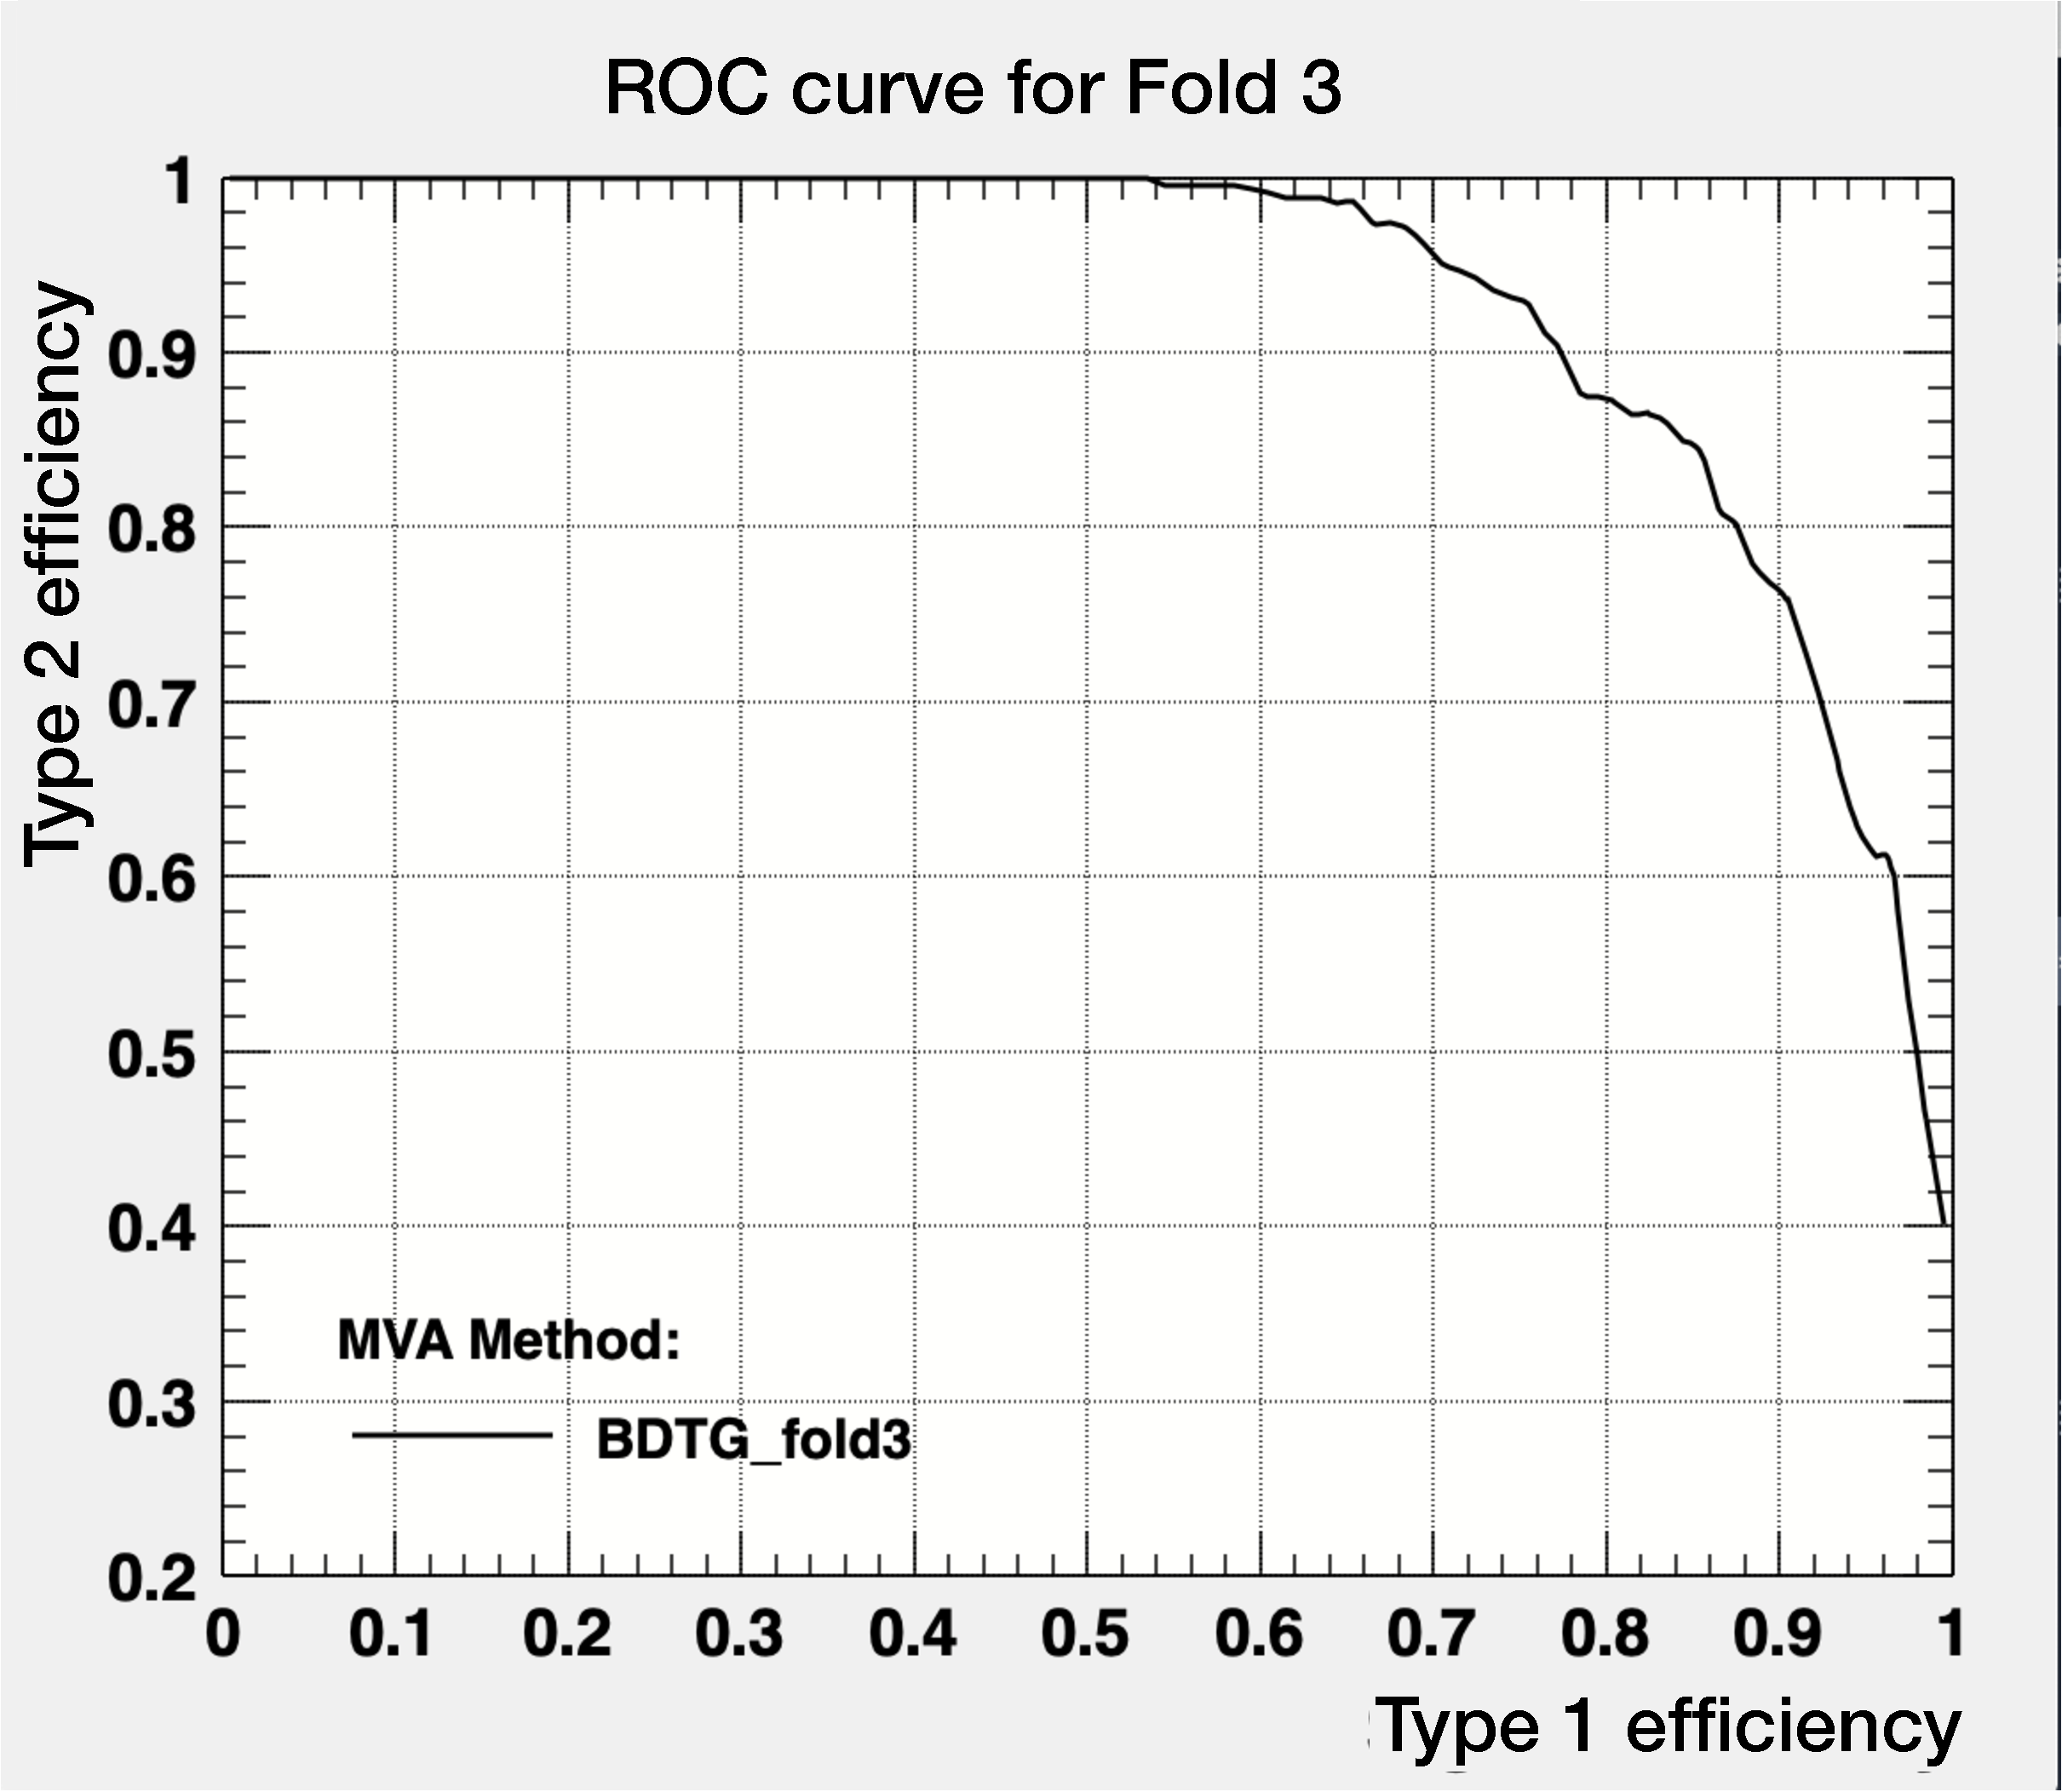
\includegraphics[width=.3\textwidth]{Chapter5_tHq/LeptAssociation/dileptau_ROC_Curve_Fold3}
\medskip
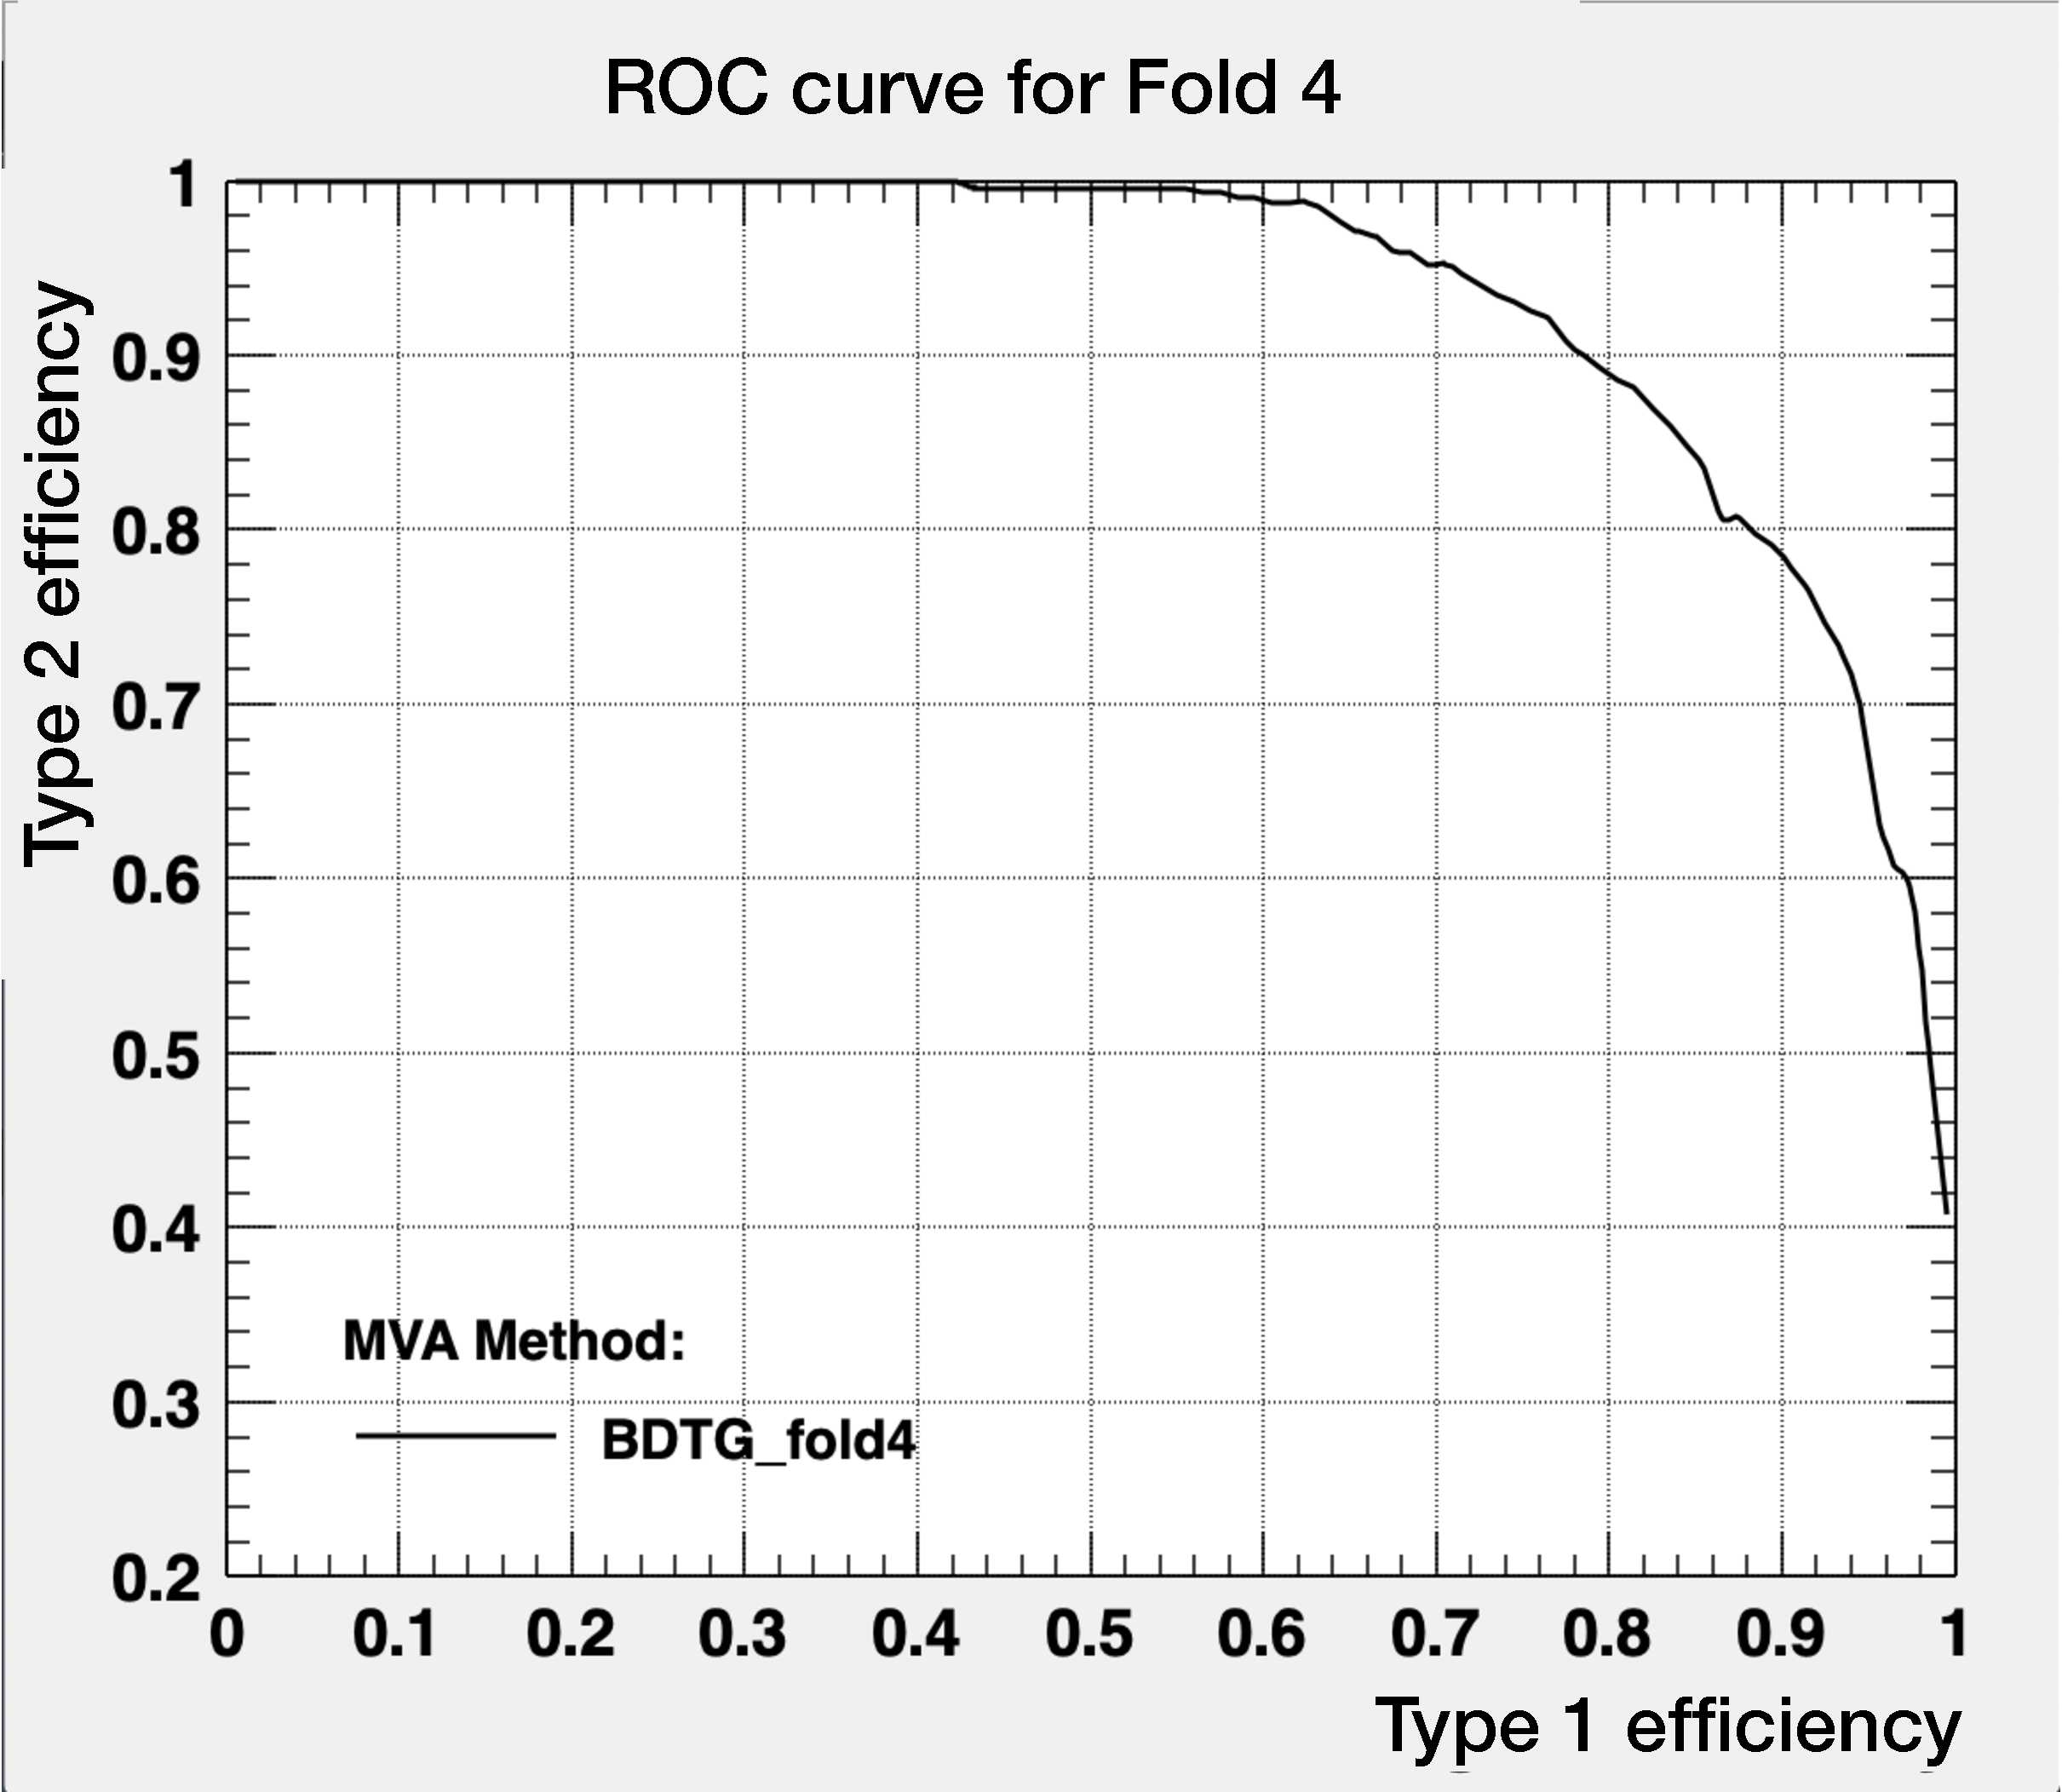
\includegraphics[width=.3\textwidth]{Chapter5_tHq/LeptAssociation/dileptau_ROC_Curve_Fold4}\quad
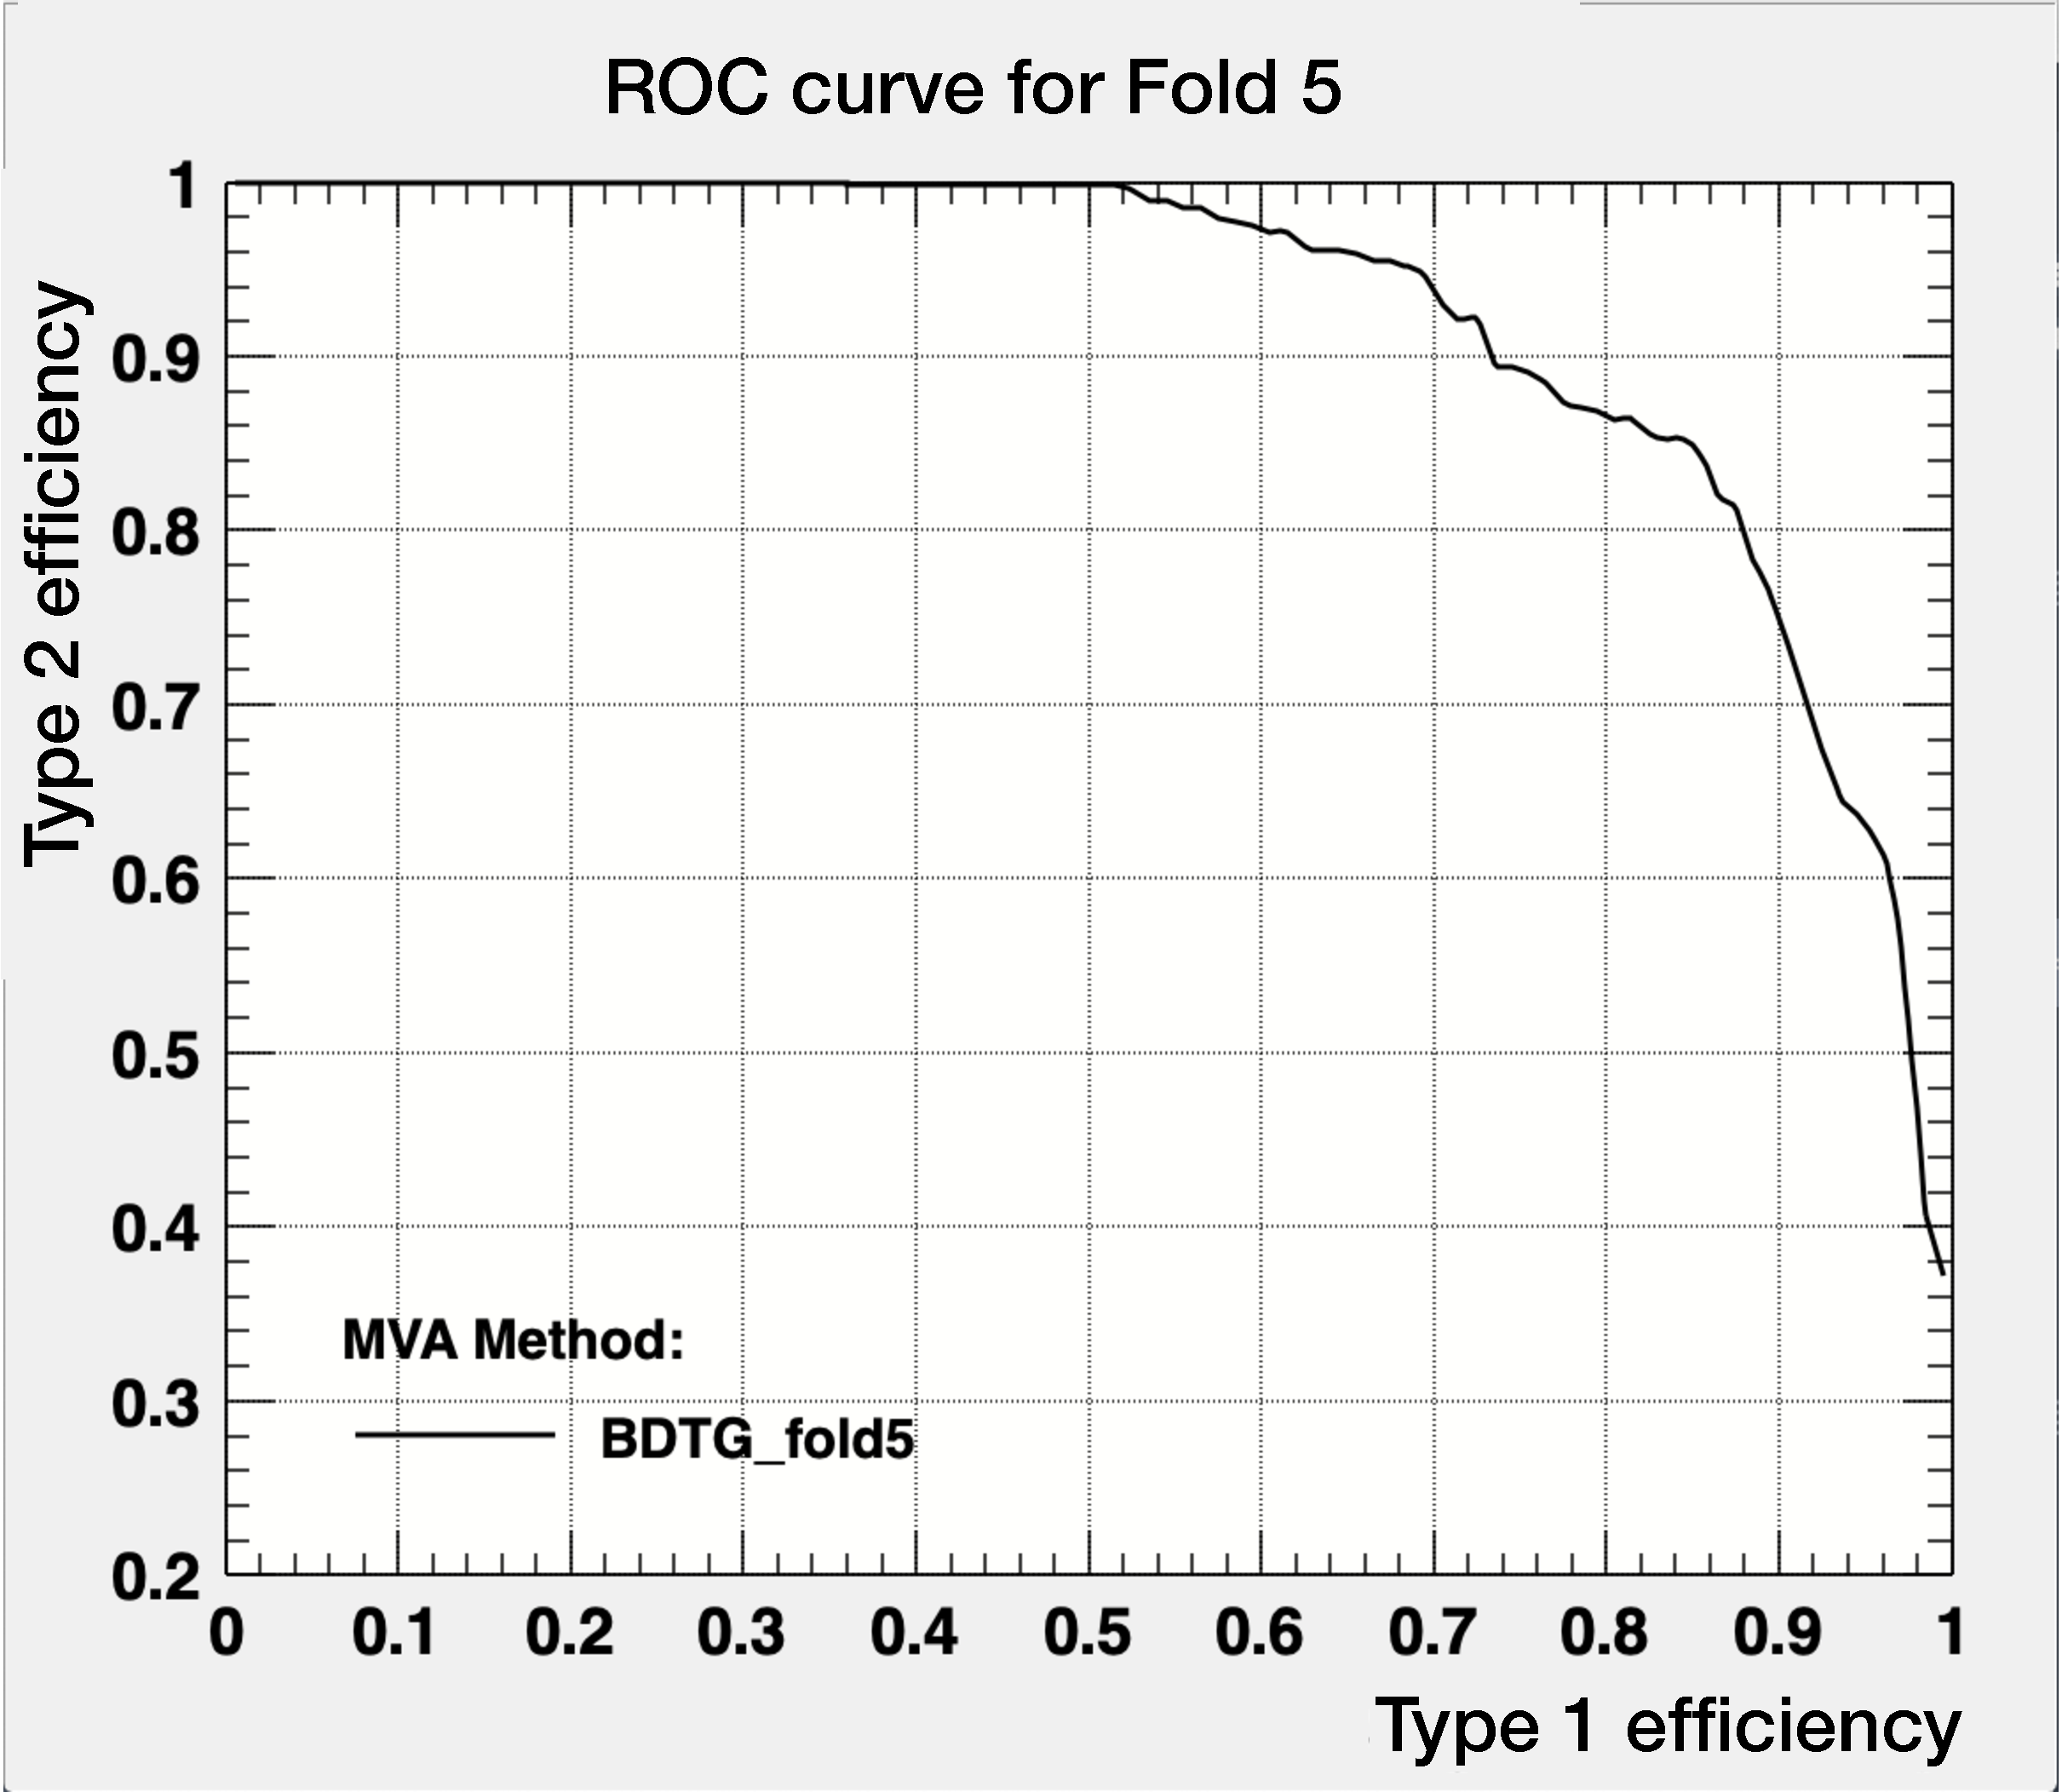
\includegraphics[width=.3\textwidth]{Chapter5_tHq/LeptAssociation/dileptau_ROC_Curve_Fold5}
\caption{ROC for the five different BDTs trained with k-folding for the $\text{BDT}^{\text{Lepton Assignment}}$ in Section~\ref{sec:ChaptH:Sig:LepAsign}.
All the curves show a similar behaviour.}
\label{fig:dileptau:Assignment_appendix:ROCs}
\end{figure}


%\begin{table}[]
%\centering
%\resizebox{\textwidth}{!}{
%\begin{tabular}{l|lllllllllllllllllllllllllll}
%\toprule
%BDT point         & -0.45 &    -0.4 &  -0.35 &  -0.33 & -0.32  & -0.315 & -0.31 & -0.395 & -0.3    & -0.29 & -0.28 & -0.27 & -0.25 & -0.2 & -0.15 & -0.1 & -0.05 & 0.0 & 0.05 & 0.1 & 0.15 & 0.2 & 0.25 & 0.3 & 0.35 & 0.4 & 0.45 \\ \midrule
%Accuracy (\%)  & 88.12 & 88.03 & 87.97 & 88.23 & 88.33 & 88.39  & 88.36 & 88.32  & 88.15 & 87.85 & 87.89 & 87.99 & 87.84 & 87.62 & 87.47 & 86.87 & 86.84 & 86.57 & 86.57 & 86.6 & 86.22 & 86.81 & 86.56 & 86.15 & 86.12 & 85.22 & 84.77  \\
%\bottomrule   
%\end{tabular}}
%\caption{Different thresholds for lepton association compared to its correspondent accuracy.}
%\label{tab:dileptau:Assignment_appendix:Thereshold_large}
%\end{table}



%%%%%%% Extra plots ::   Region definition
\subsection{BDTs for region definition}
\label{sec:BDT:AdditionalMaterial:Region}
The three BDTs used to define the analysis regions are presented in 
Section~\ref{sec:ChaptH:EventSelection:BDT}. Two of these are
trained on \dilepOStau events to target the signal and the \ttbar 
process. These are the BDT$(\tHq|_{\text{OS}})$ and BDT$(\ttbar|_{\text{OS}})$,
respectively. For the \dilepSStau channel, only one BDT is used for the analysis,
the BDT$(\tHq|_{\text{SS}})$, which targets the signal.  In this section, 
the correlations between the variables of each model are presented first.
Then, the training evolution is studied with the AUC and LogLoss progression
over the training epochs.

%%%%%%% Extra plots ::   Region definition - Correlations
\subsection{Correlation between input features}
\label{sec:BDT:AdditionalMaterial:Region:Correlations}
When choosing the input variables of an ML model, it is important to check for correlations 
between these variables because highly correlated variables can lead to redundancy, 
reducing the efficiency and interpretability of the model. This helps to avoid overfitting, 
ensuring the model generalises well to new, unseen data. 
For the feature selection described in Section~\ref{sec:ChaptH:EventSelection:BDT:Variables},
the linear correlations among all variables within a model have
been explored and the results are presented in Figures~\ref{fig:ChaptH:EventSelection:BDT:Correlation:tHqOS},
\ref{fig:ChaptH:EventSelection:BDT:Correlation:ttbarOS} and~\ref{fig:ChaptH:EventSelection:BDT:Correlation:tHqSS}.
In these figures, the more intense the colour, the higher the correlation. 
For the BDT$(\tHq|_{\text{OS}})$ is of particular relevance the correlation between the 
$\Delta \eta ($forward non-$b$-tagged jet, subleading $b$-tagged jet$)$ and the multiplicity
of forward jets. These two variables have a correlation of 87\% and 85\% for the signal and the
background, respectively, so it could be beneficial to remove one of these two. 
For the BDT$(\ttbar|_{\text{OS}})$ model there is not any highly correlated pair of variables, being
the highest correlation a 52\%. 
Similarly, for the BDT$(\tHq|_{\text{SS}})$, the only correlation appears for the \pT and the energy
of the top quark. Since the energy depends on the momentum, it is not surprising that these two
present a 66\% (\ttbar) and 72\% (other processes) correlation.



\begin{figure}[h]
\centering
\begin{subfigure}{.475\textwidth}
  \centering
  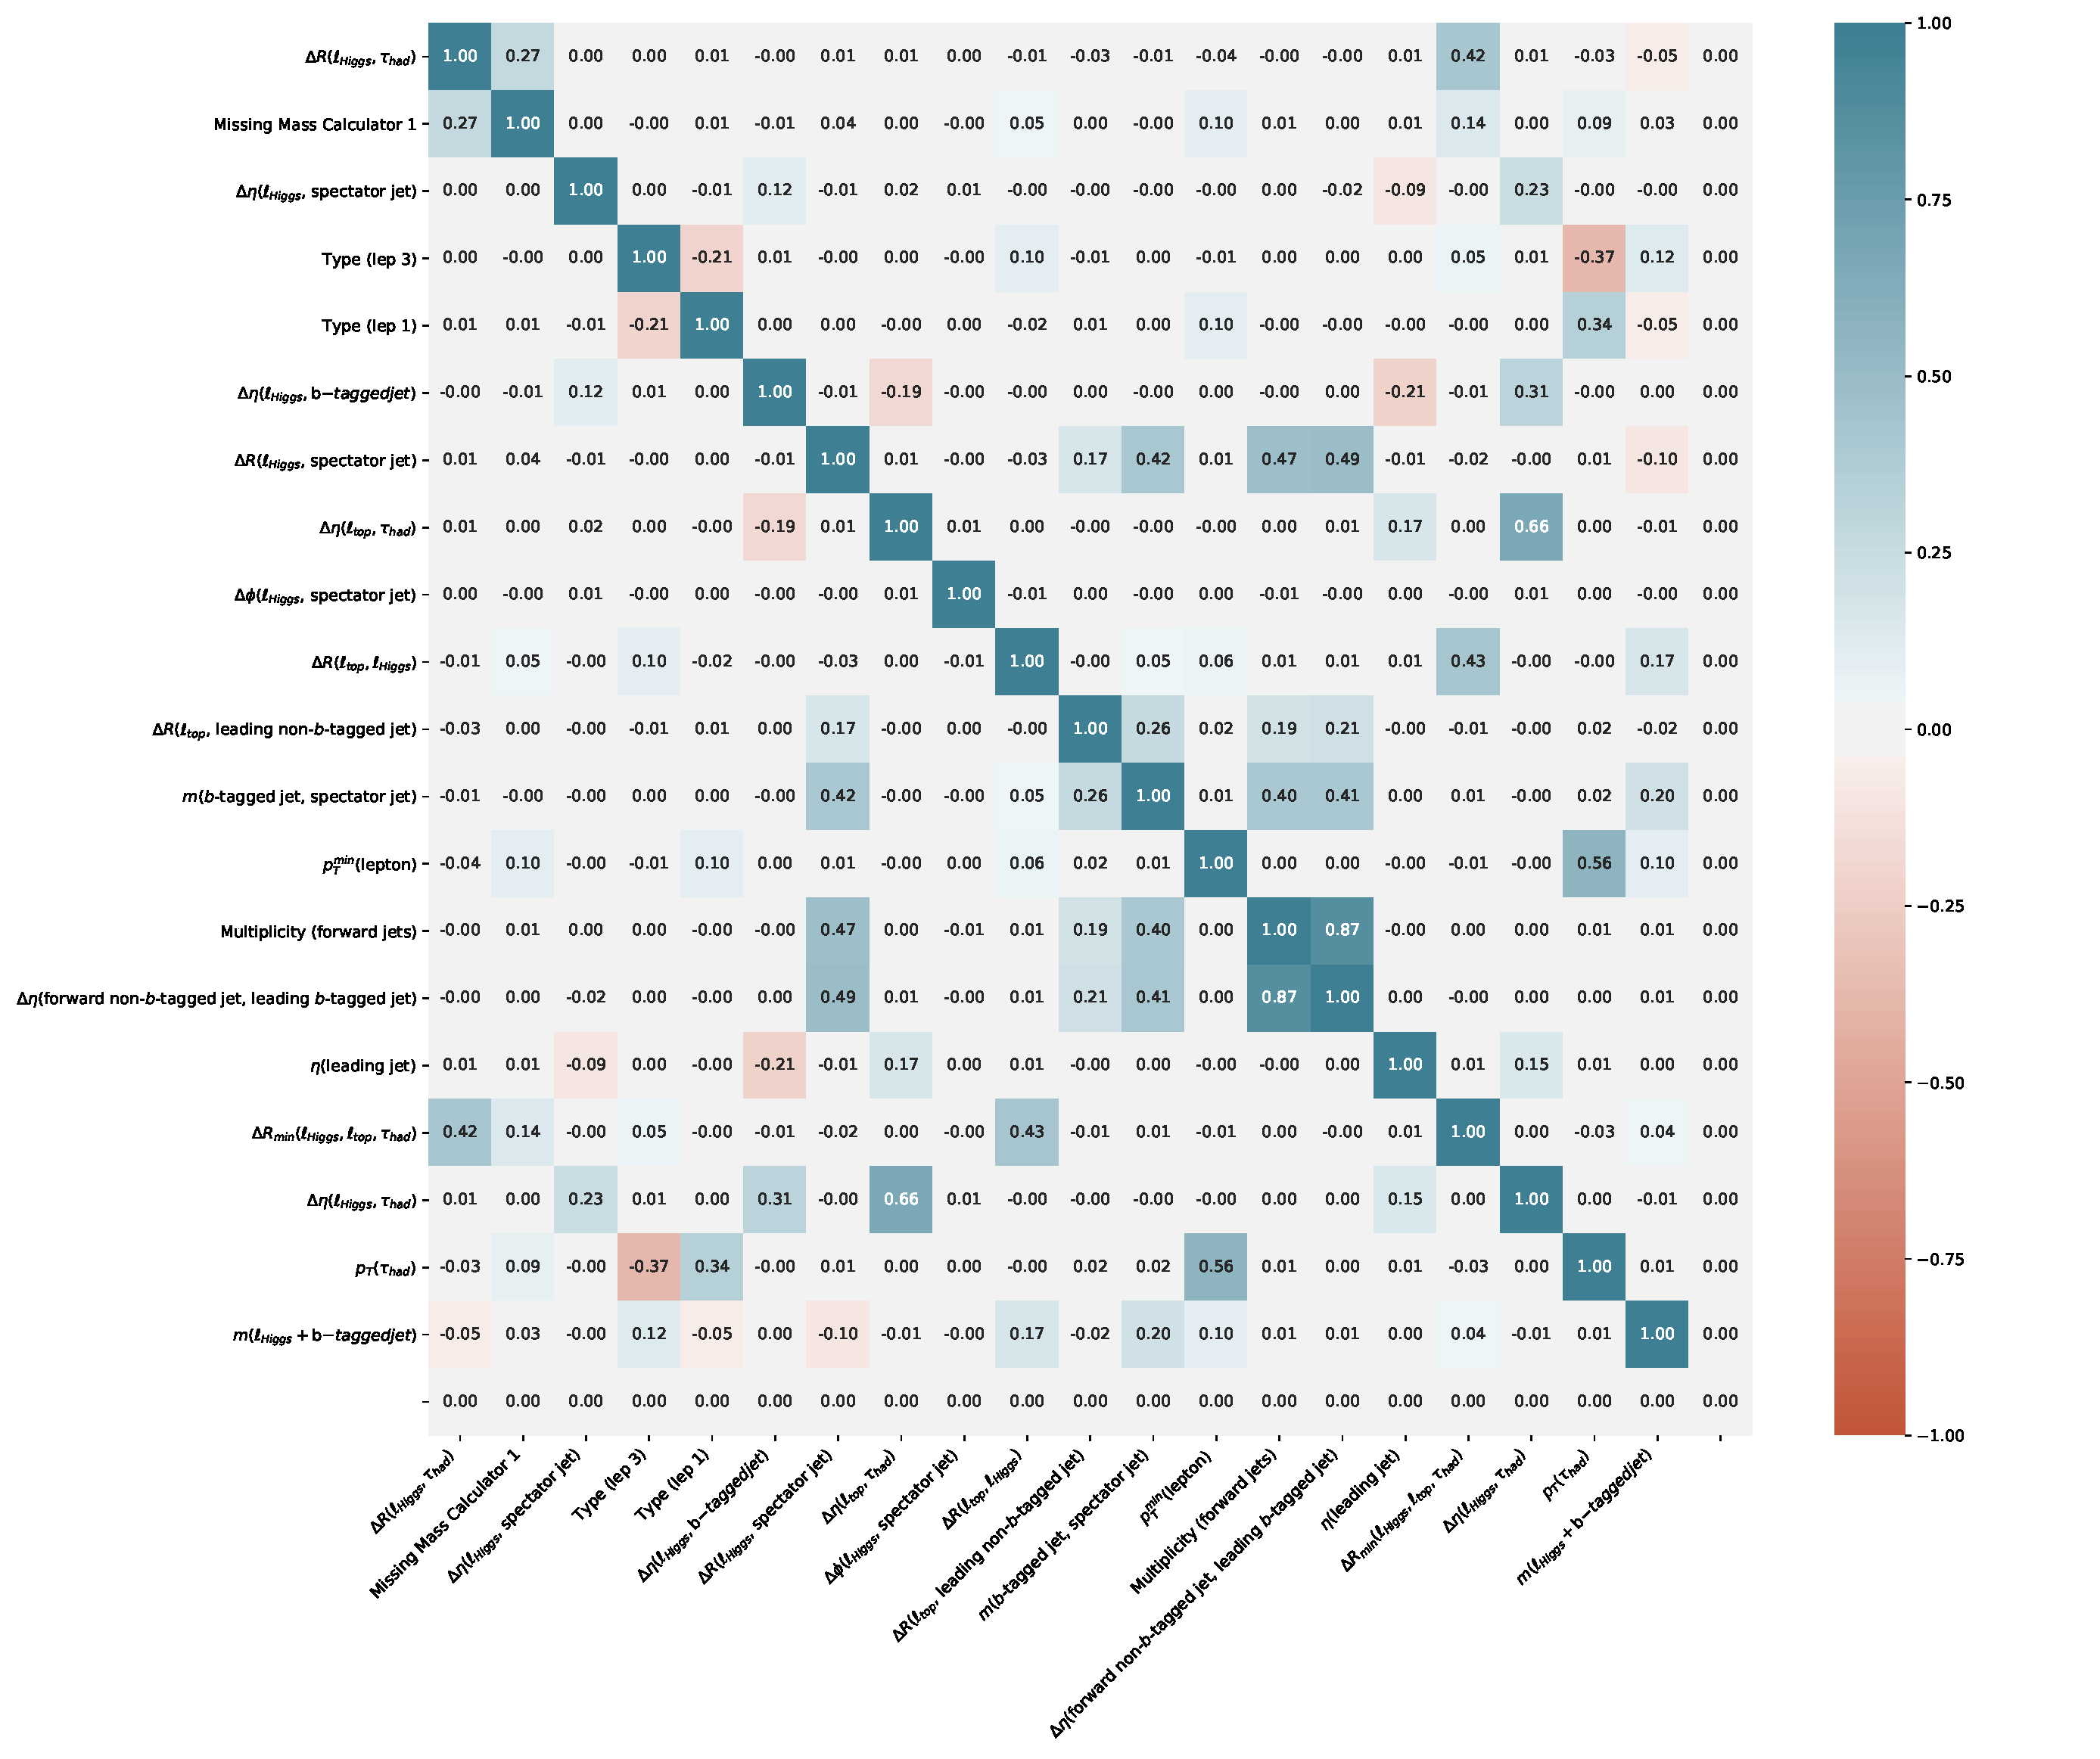
\includegraphics[width=.9\linewidth]{Chapter5_tHq/BDT_Results/correlation_number_2LOSTau_BDT_Target_tHq}
  \label{fig:ChaptH:EventSelection:BDT:Correlation:tHqOS:target}
\end{subfigure}%
\begin{subfigure}{.475\textwidth}
  \centering
  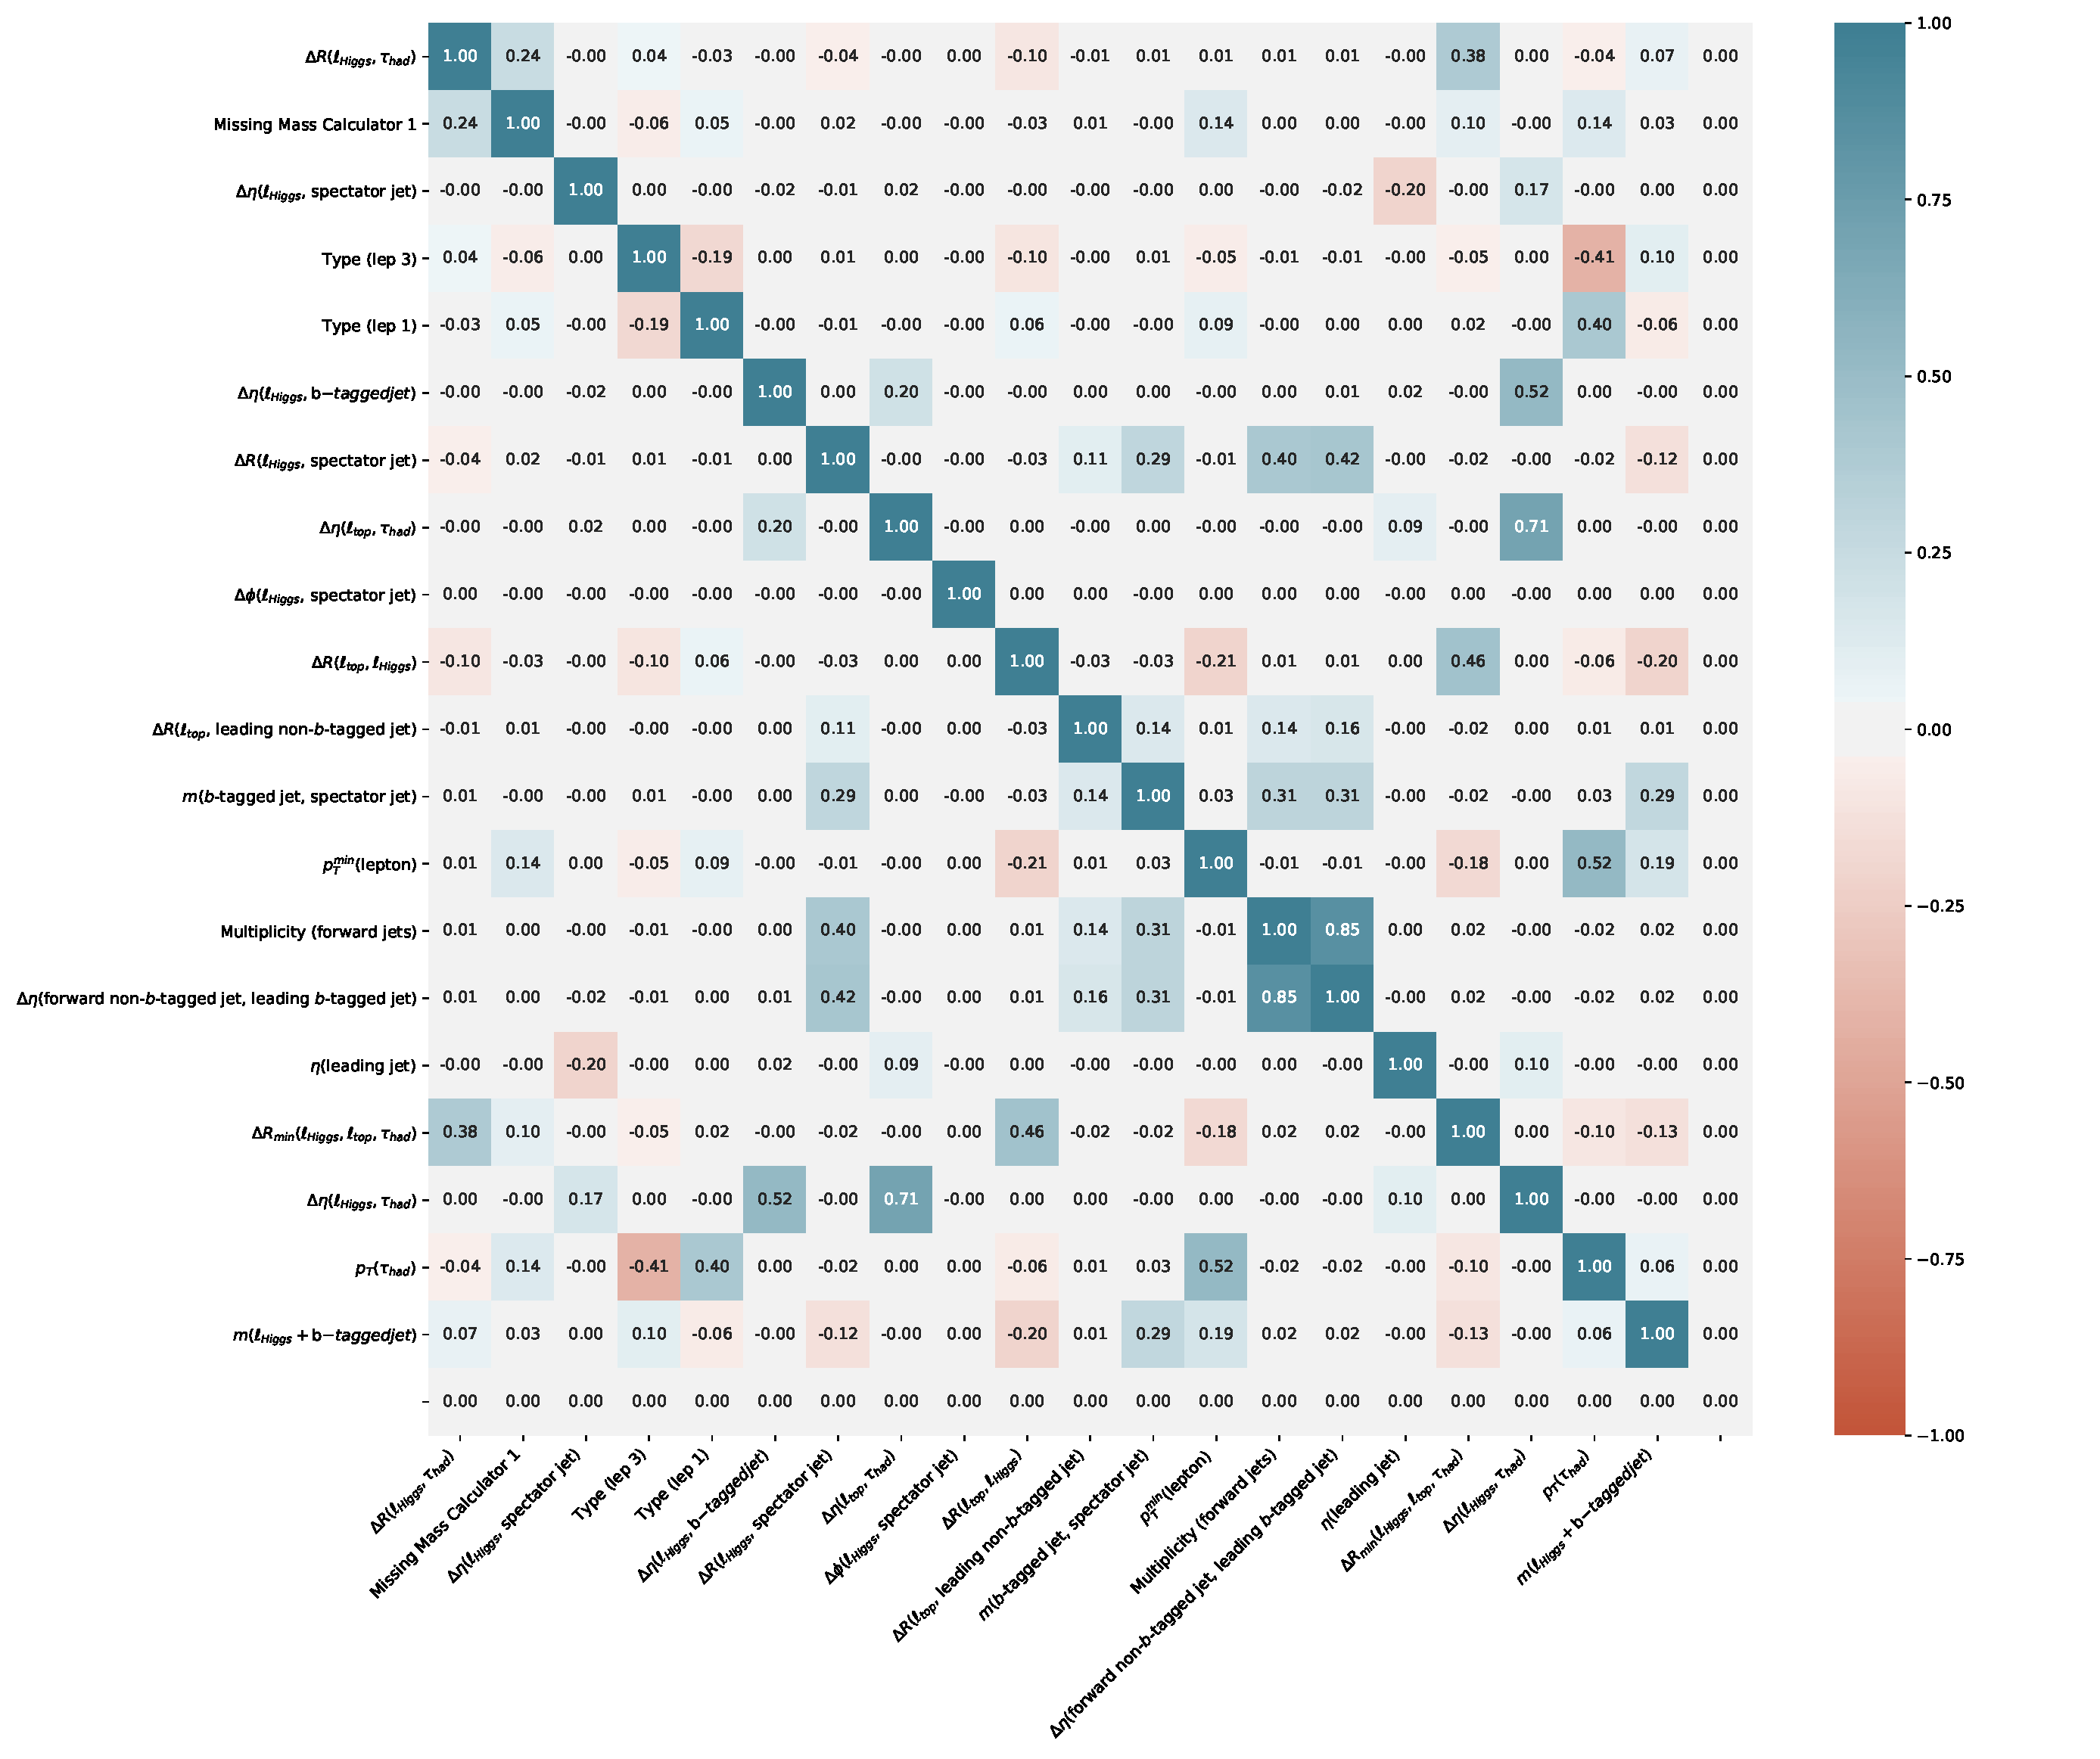
\includegraphics[width=.9\linewidth]{Chapter5_tHq/BDT_Results/correlation_number_2LOSTau_BDT_OthersThan_tHq}
  \label{fig:ChaptH:EventSelection:BDT:Correlation:tHqOS:rest}
\end{subfigure}
\caption{Correlation matrix of the variables used as input in the BDT$(\tHq|_{\text{OS}})$. 
For the left matrix, the correlations among variables are explored for the \tHq process only while, for the right plot, these
are studied for all the backgrounds. Correlations are presented in blue while anticorrelations are in orange.}
\label{fig:ChaptH:EventSelection:BDT:Correlation:tHqOS}
\end{figure}


\begin{figure}[h]
\centering
\begin{subfigure}{.475\textwidth}
  \centering
  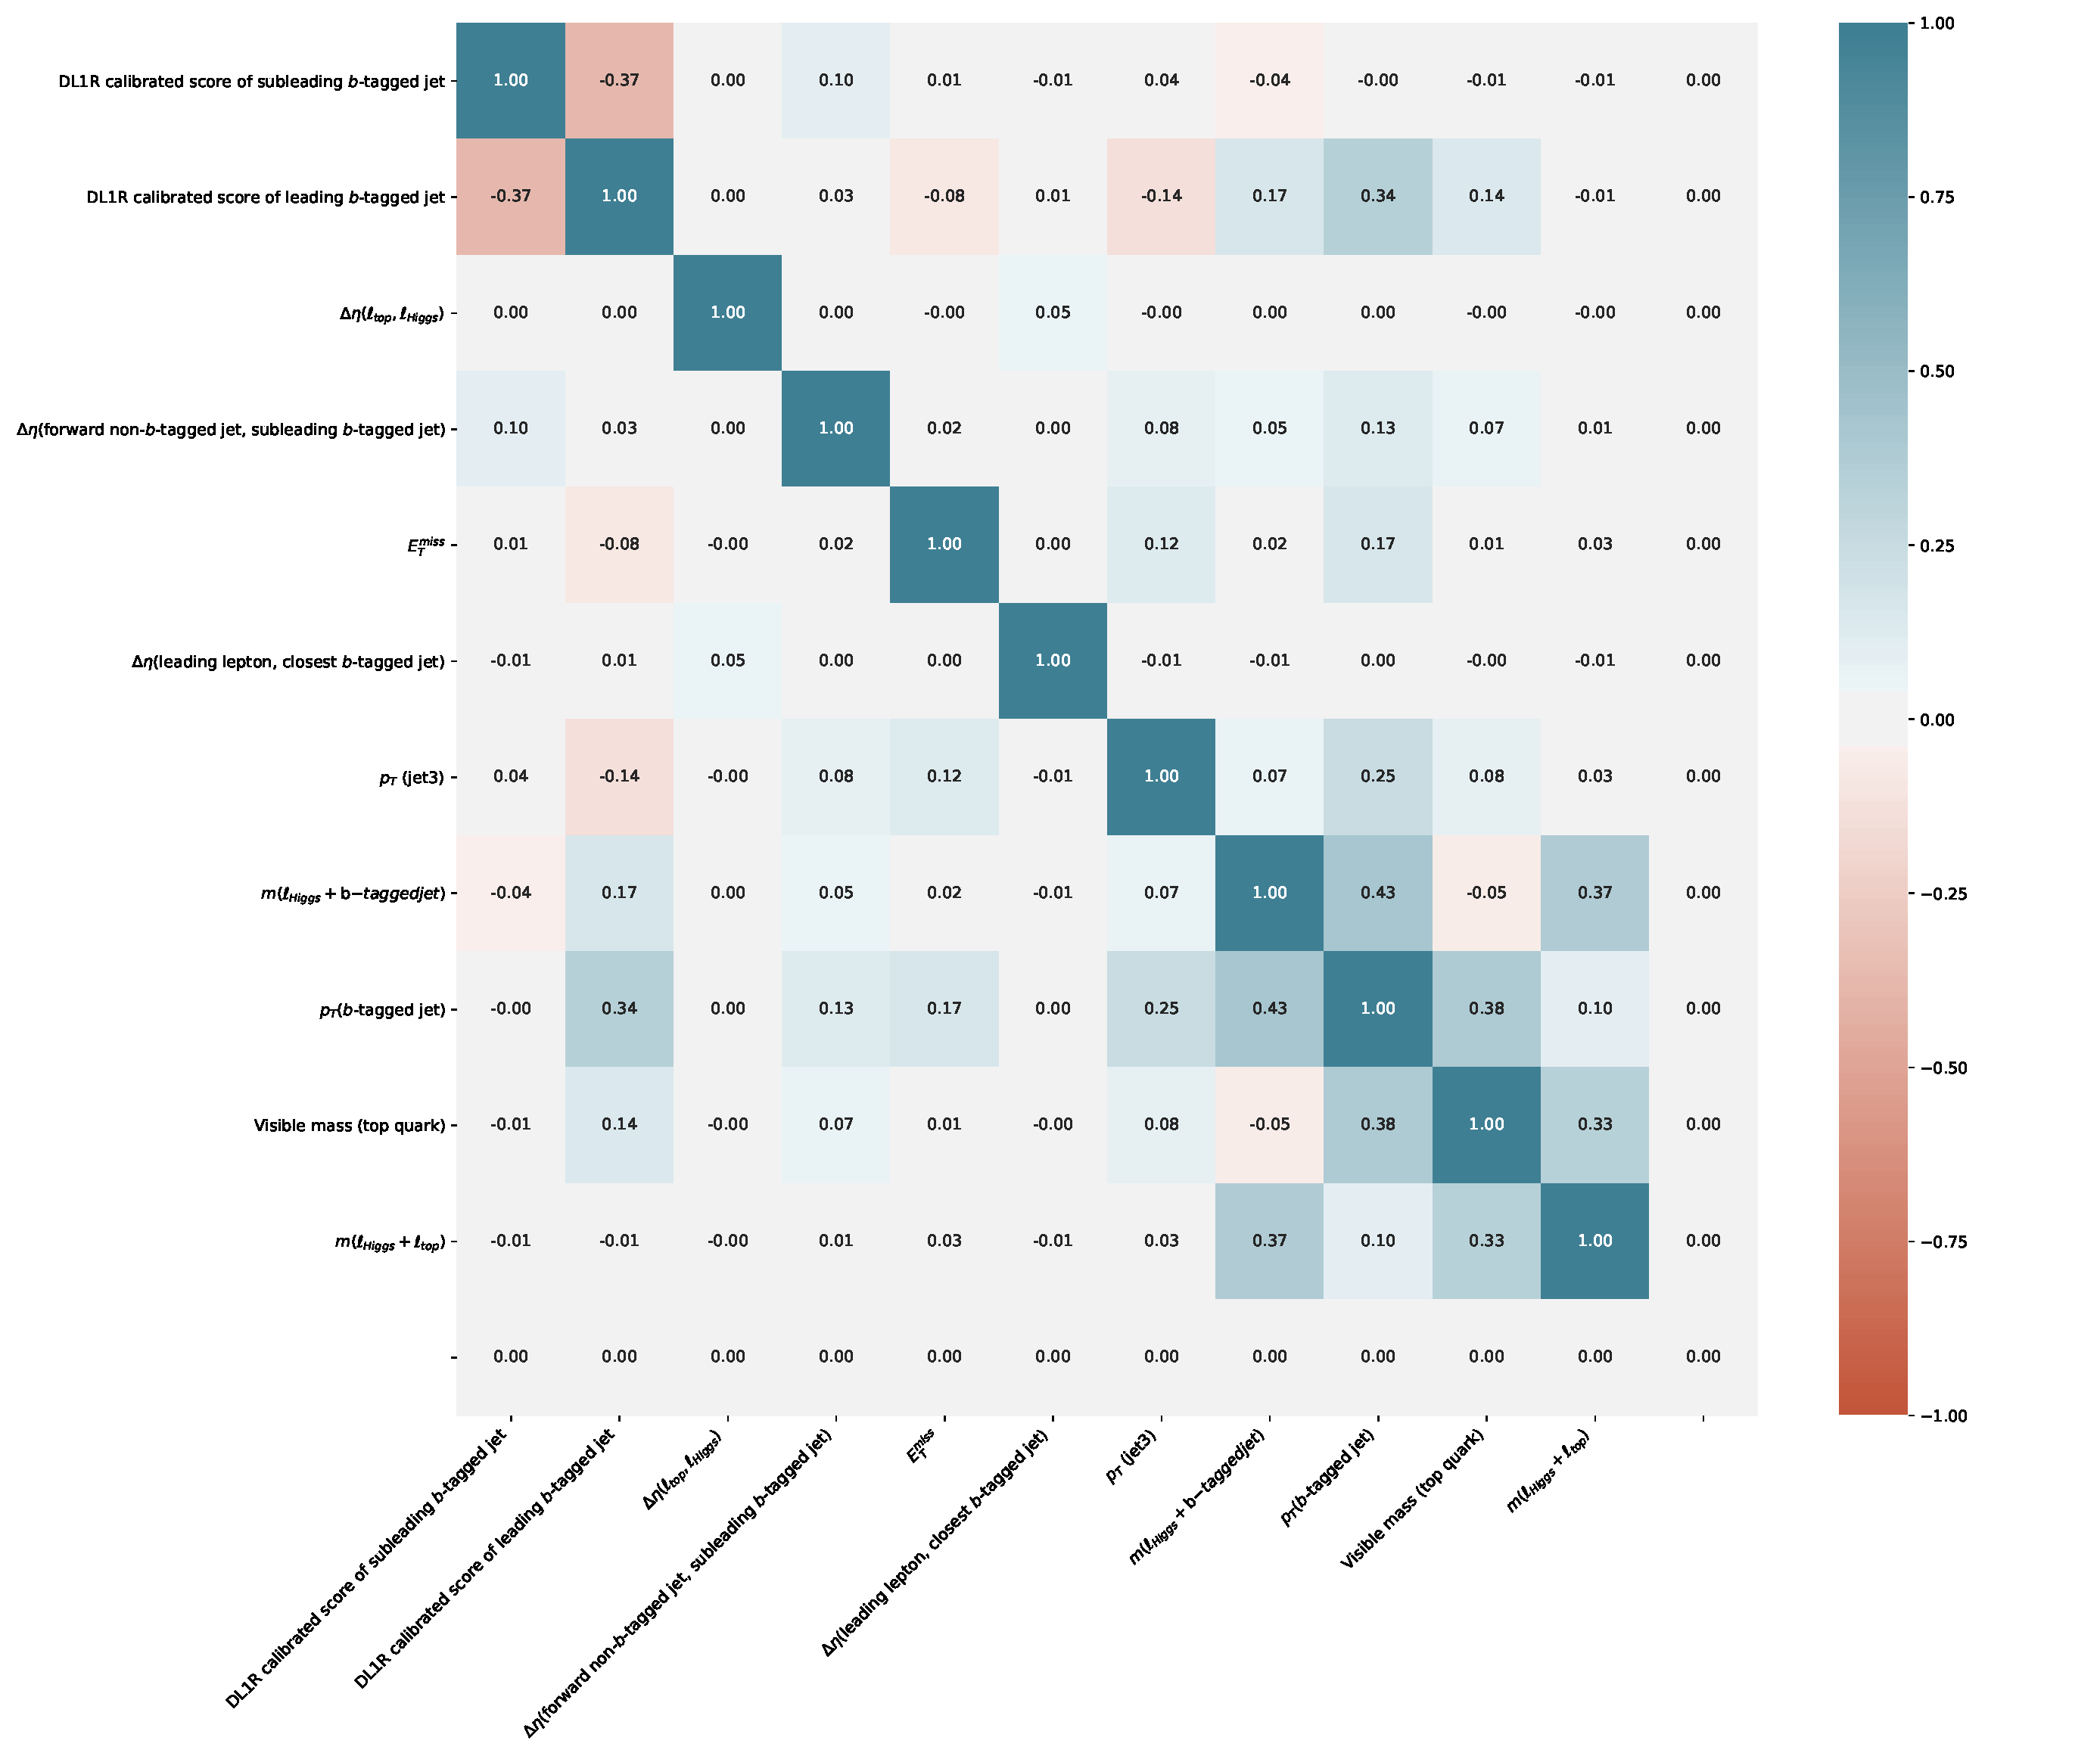
\includegraphics[width=.9\linewidth]{Chapter5_tHq/BDT_Results/correlation_number_2LOSTau_BDT_Target_ttbar}
  \label{fig:ChaptH:EventSelection:BDT:Correlation:ttbarOS:target}
\end{subfigure}%
\begin{subfigure}{.475\textwidth}
  \centering
  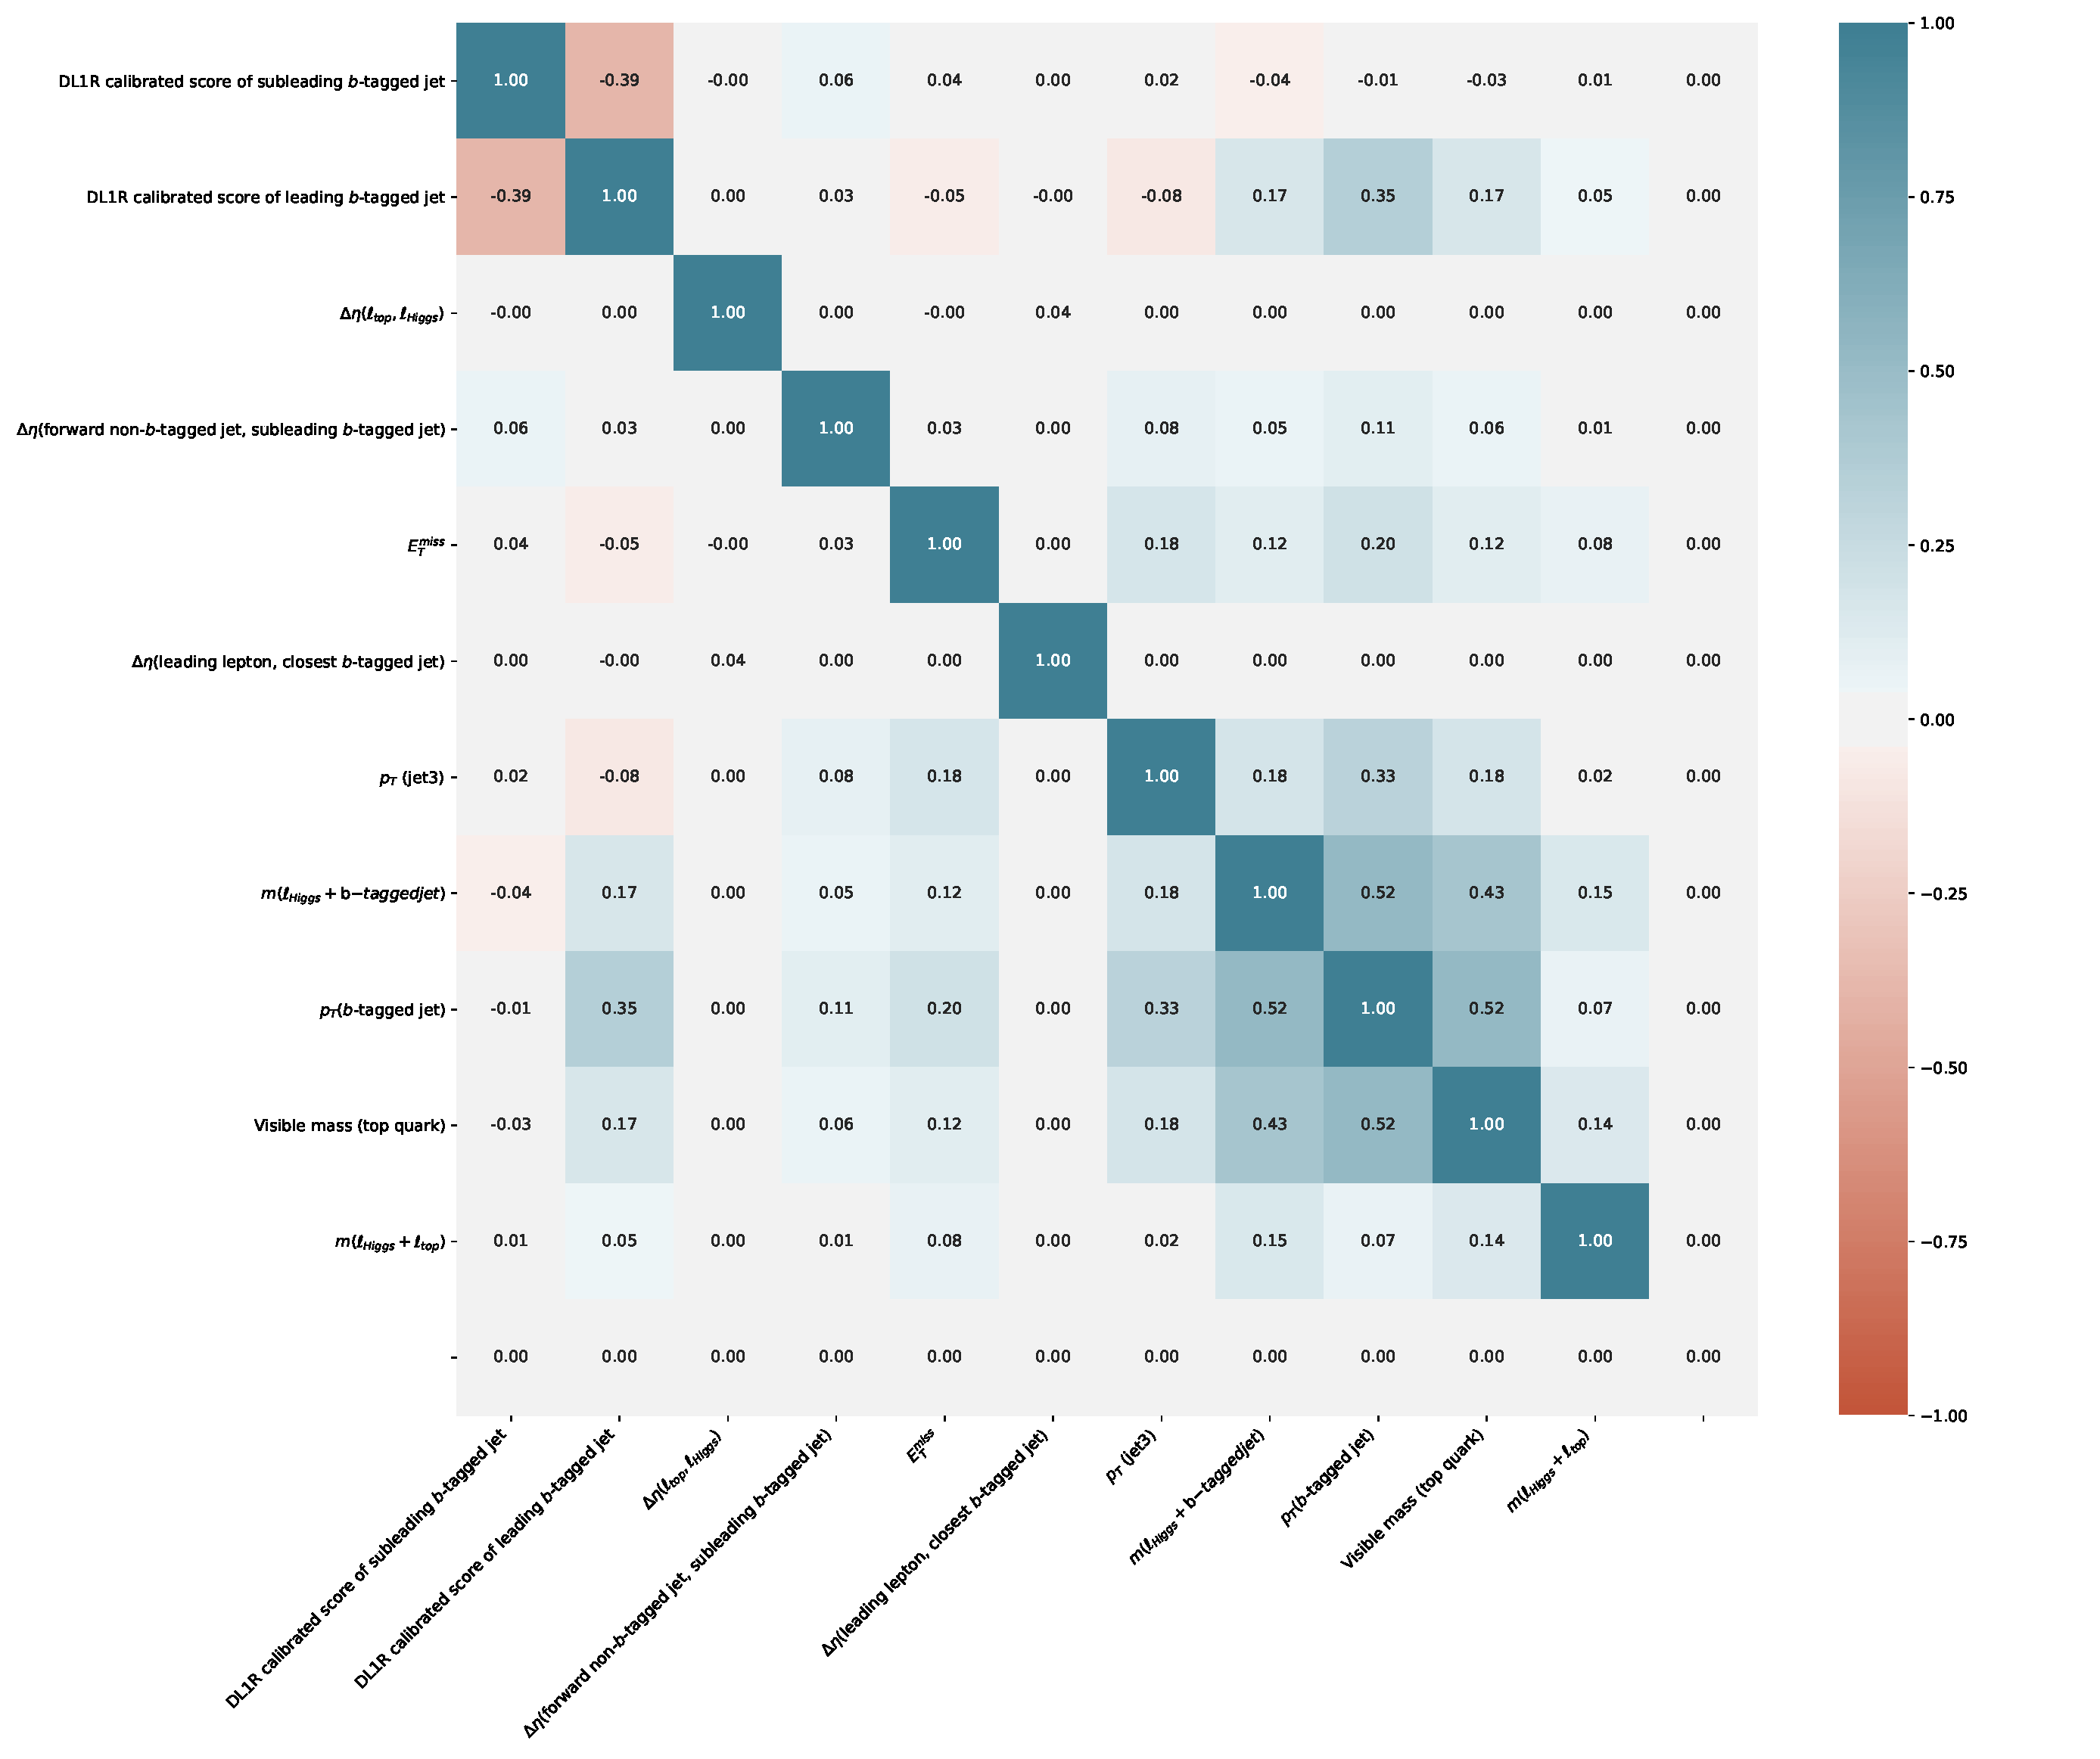
\includegraphics[width=.9\linewidth]{Chapter5_tHq/BDT_Results/correlation_number_2LOSTau_BDT_OthersThan_ttbar}
  \label{fig:ChaptH:EventSelection:BDT:Correlation:ttbarOS:rest}
\end{subfigure}
\caption{Correlation matrix of the variables used as input in the BDT$(\ttbar|_{\text{OS}})$. 
For the left matrix, the correlations among variables are explored for the \ttbar process only while, for the right plot, the
correlations are calculated for the other processes. Only linear correlations are shown and higher-order relationships may not
be reflected in this matrix.}
\label{fig:ChaptH:EventSelection:BDT:Correlation:ttbarOS}
\end{figure}


\begin{figure}[h]
\centering
\begin{subfigure}{.475\textwidth}
  \centering
  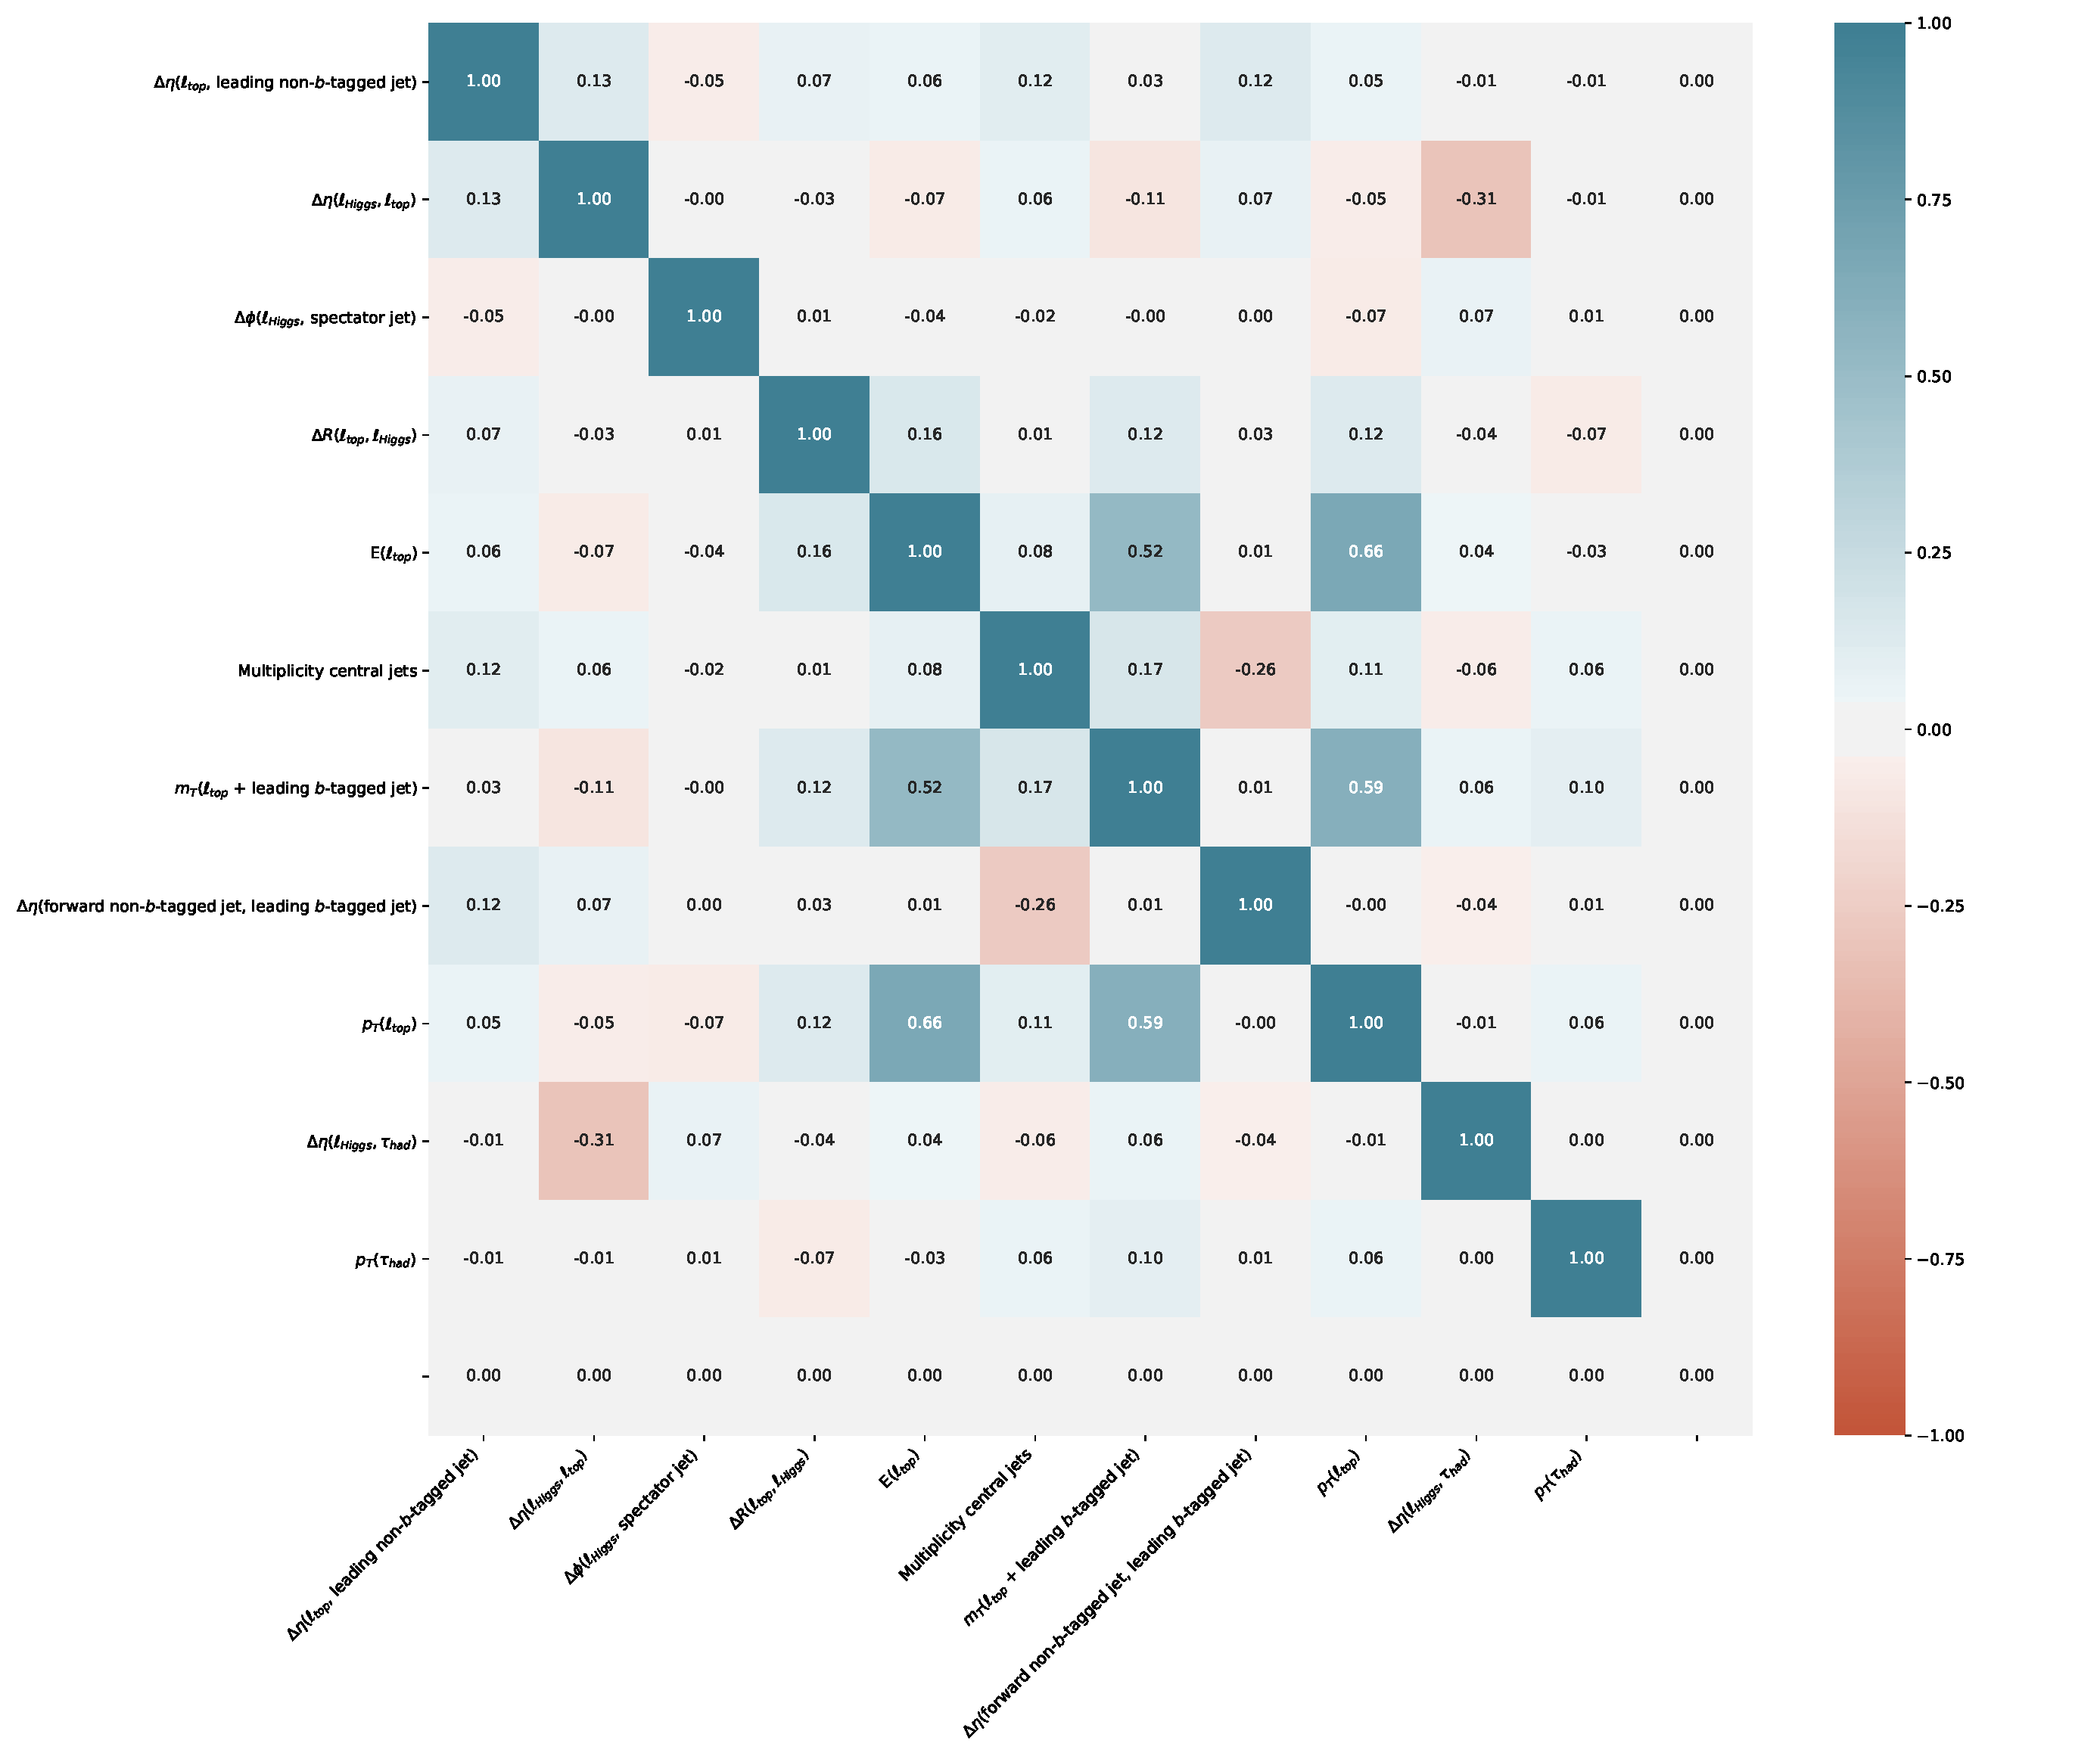
\includegraphics[width=.9\linewidth]{Chapter5_tHq/BDT_Results/correlation_number_2LSSTau_BDT_Target_tHq}
  \label{fig:ChaptH:EventSelection:BDT:Correlation:tHqSS:target}
\end{subfigure}%
\begin{subfigure}{.475\textwidth}
  \centering
  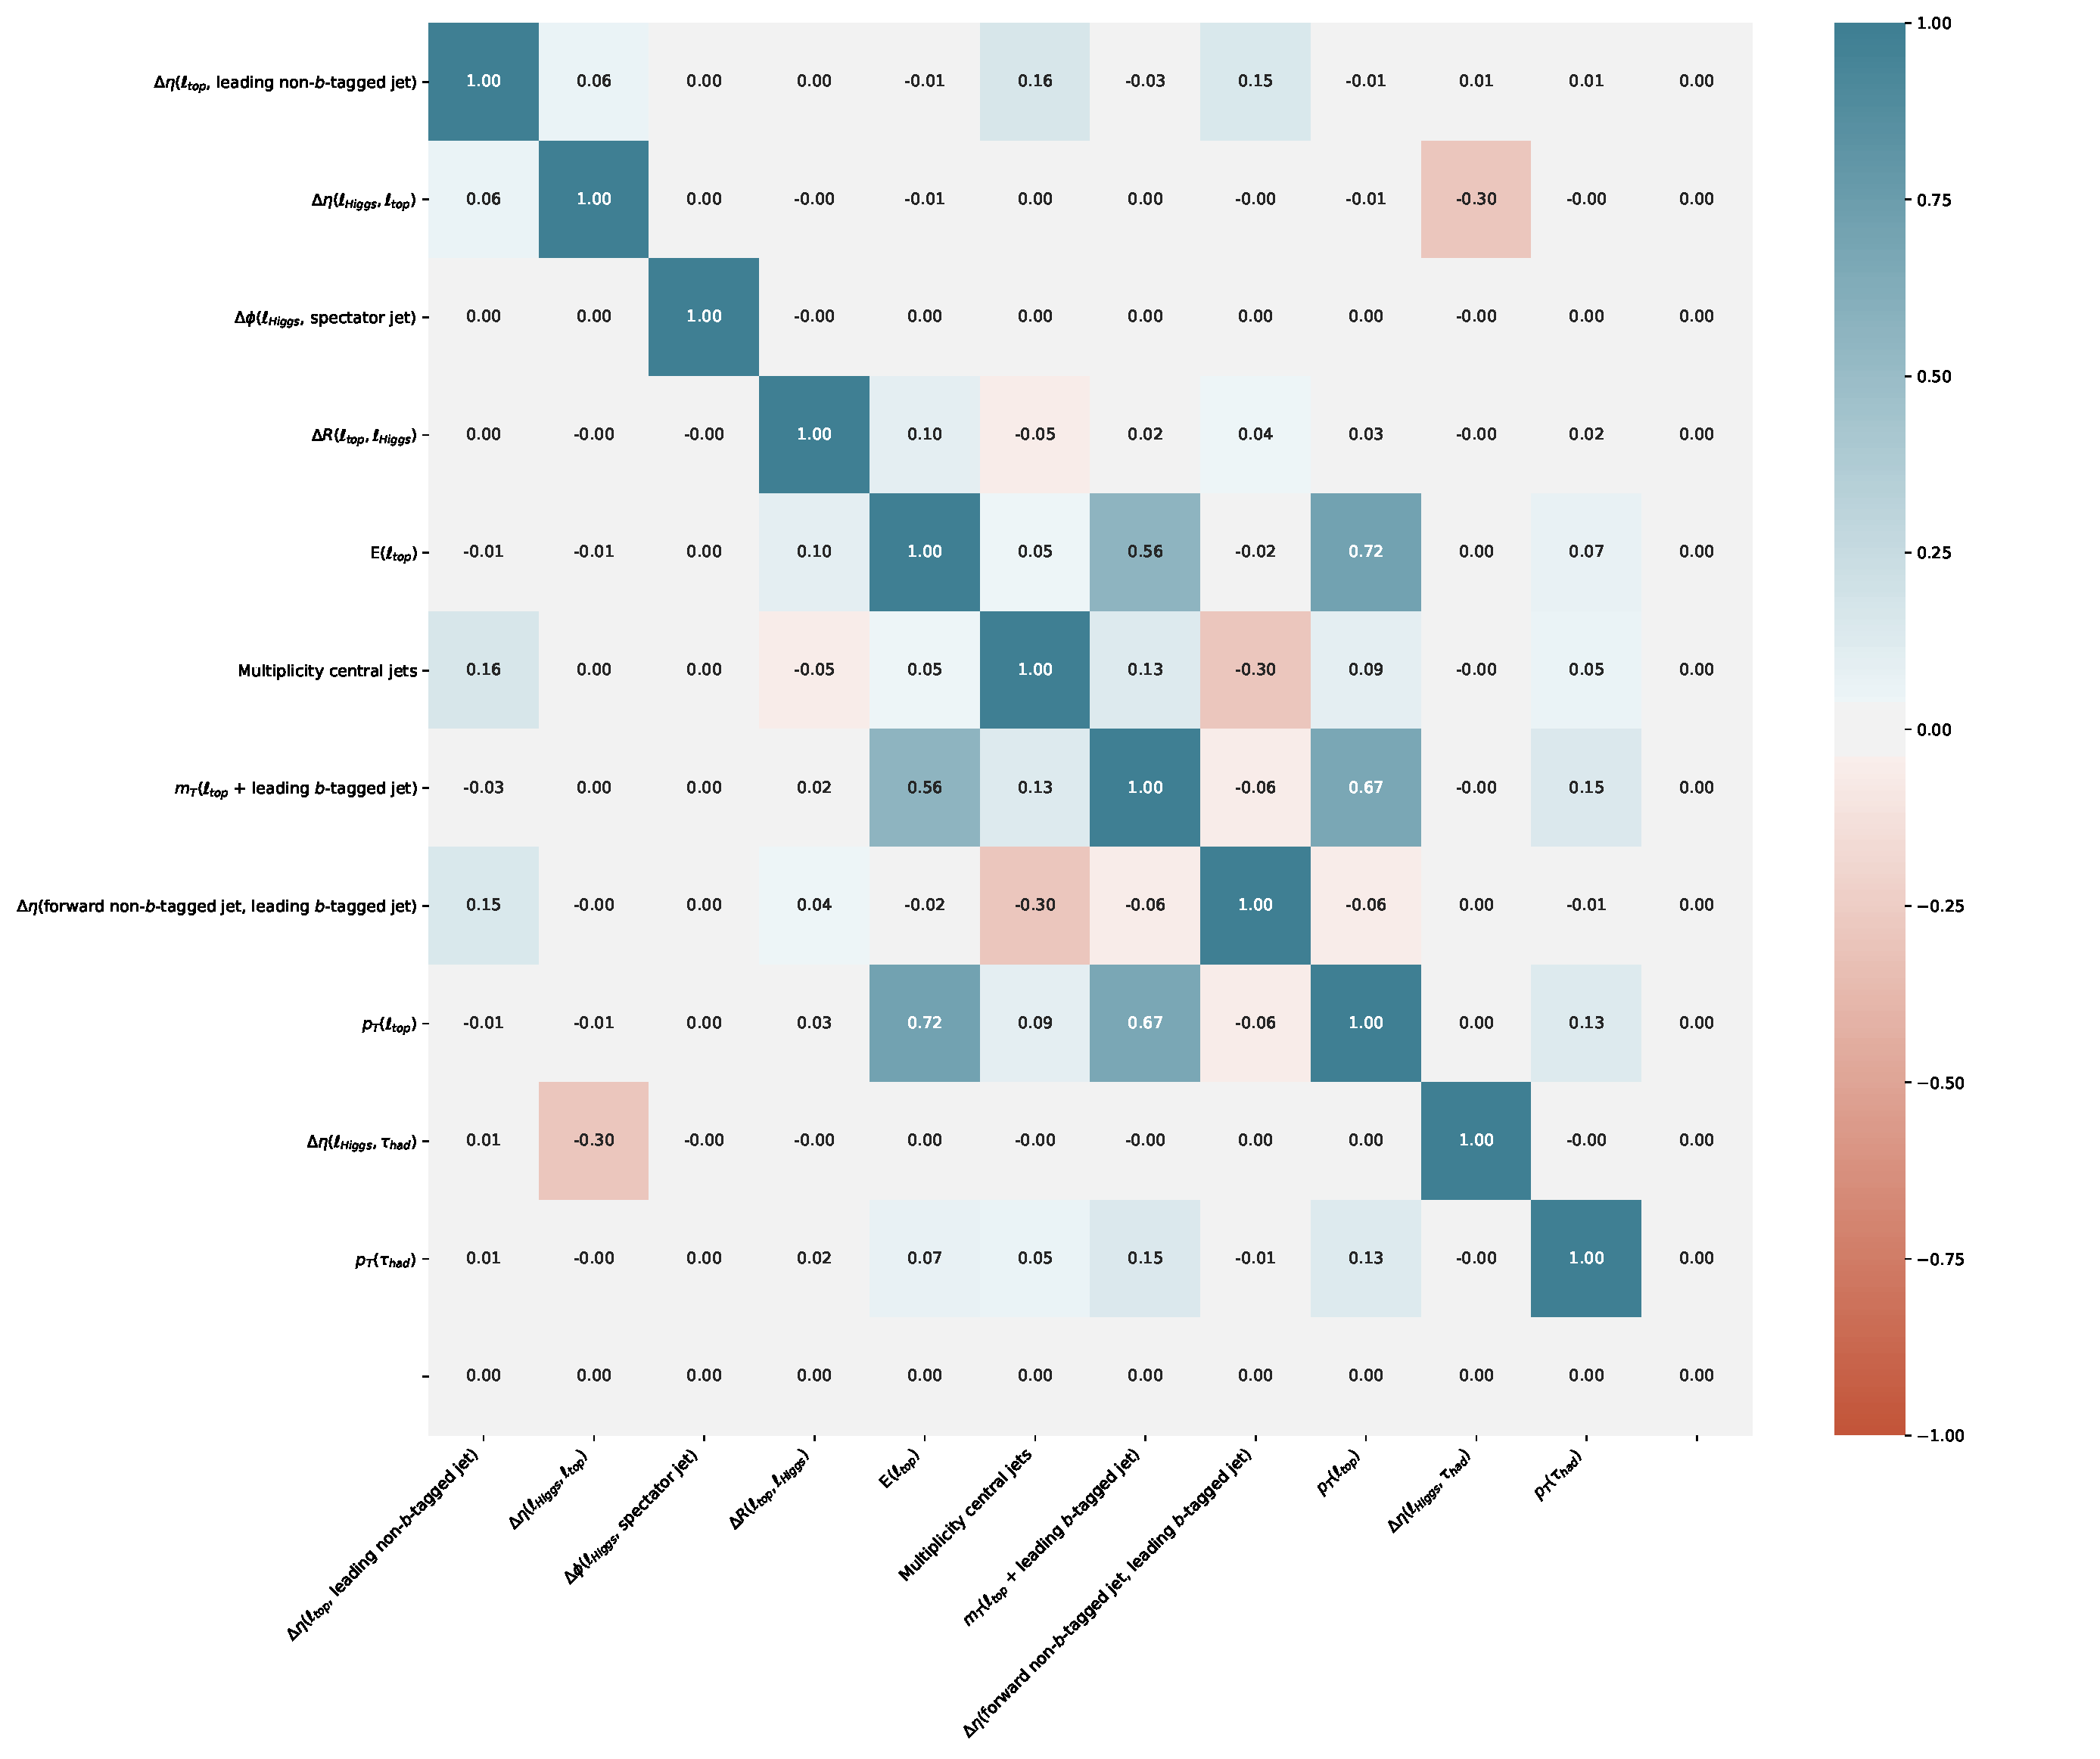
\includegraphics[width=.9\linewidth]{Chapter5_tHq/BDT_Results/correlation_number_2LSSTau_BDT_OthersThan_tHq}
  \label{fig:ChaptH:EventSelection:BDT:Correlation:tHqSS:rest}
\end{subfigure}
\caption{Correlation matrix of the variables used as input in the BDT$(\tHq|_{\text{SS}})$. 
For the left matrix, the correlations among variables are explored for the \tHq process only while, for the right plot, these
are studied for the background processes.}
\label{fig:ChaptH:EventSelection:BDT:Correlation:tHqSS}
\end{figure}


%%%%%%% Extra plots ::   Region definition - Evolution
\subsection{Evolution of training}
\label{sec:BDT:AdditionalMaterial:Region:Evolution}
The loss values of the training and test offer a deeper understanding of how learning performance 
evolves across different epochs. These metrics provide useful insight into how the learning performance 
changes over the number of epochs. This can help diagnose potential learning issues that might 
result in an underfitted or overfitted model. %Additionally, they guide the selection of the most appropriate
%epoch for using the trained model weights during the inferencing stage.

Figures~\ref{fig:ChaptH:EventSelection:BDT:Epochs:tHqOS},~\ref{fig:ChaptH:EventSelection:BDT:Epochs:ttbarOS} 
and~\ref{fig:ChaptH:EventSelection:BDT:Epochs:tHqSS} present the
evolution of the AUC and LogLoss functions at each iteration of the training procedure. 
These are plotted, separately for train and test, so that overtraining can be detected.
The values for the AUC and LogLoss of the last epoch correspond to those presented
in Figure~\ref{tab:ChaptH:EventSelection:BDT:Metrics} (although small discrepancies 
can appear).
%Figures~\ref{fig:ChaptH:EventSelection:BDT:Epochs:tHqOS, fig:ChaptH:EventSelection:BDT:Epochs:ttbarOS, fig:ChaptH:EventSelection:BDT:Epochs:tHqSS}
%correspond to a single fold and not to the average).
The train and test curves in these plots are not diverging (as in the overtraining example in Figure~\ref{fig:Appendix:BDT:Overtrain}),
indicating that no overfitting is present.



\begin{figure}[h]
\centering
\begin{subfigure}{.475\textwidth}
  \centering
  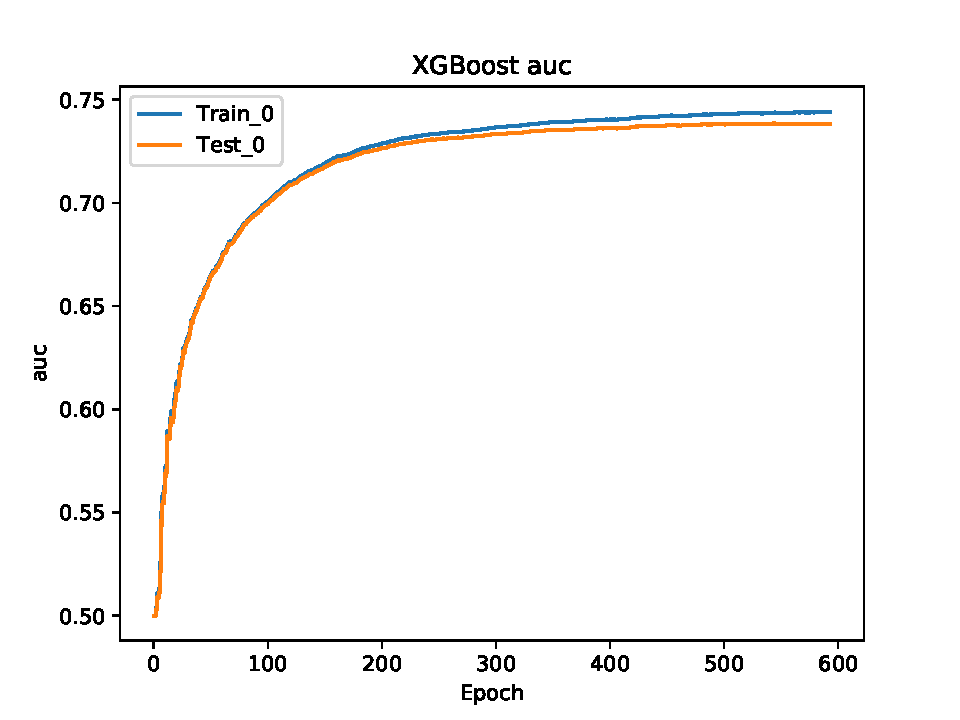
\includegraphics[width=.9\linewidth]{Appendices/BDT/Evolutionplots/auc_OS_tHq_K0}
  \caption{Area under the ROC curve.}
  \label{fig:ChaptH:EventSelection:BDT:Epochs:tHqOS:AUC}
\end{subfigure}%
\begin{subfigure}{.475\textwidth}
  \centering
  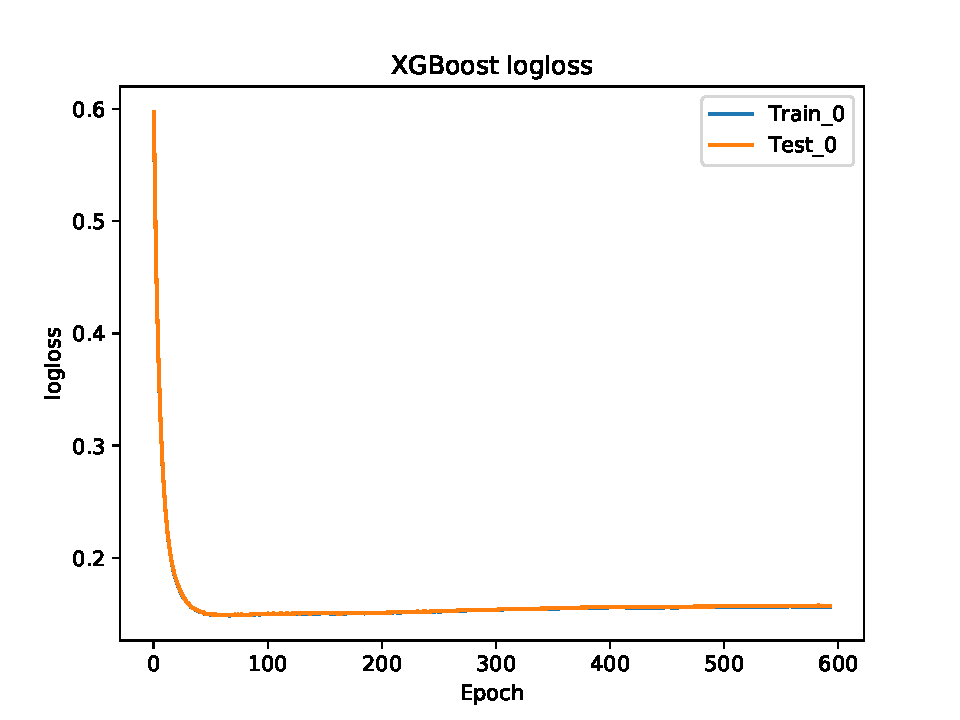
\includegraphics[width=.9\linewidth]{Appendices/BDT/Evolutionplots/logloss_OS_tHq_K0}
  \caption{Logarithm of the loss function.}
  \label{fig:ChaptH:EventSelection:BDT:Epochs:tHqOS:LogLoss}
\end{subfigure}
\caption{Evolution of the AUC and LogLoss functions for the training of the BDT$(\tHq|_{\text{OS}})$.
The x-axis shows the training iteration.}
\label{fig:ChaptH:EventSelection:BDT:Epochs:tHqOS}
\end{figure}

\begin{figure}[h]
\centering
\begin{subfigure}{.475\textwidth}
  \centering
  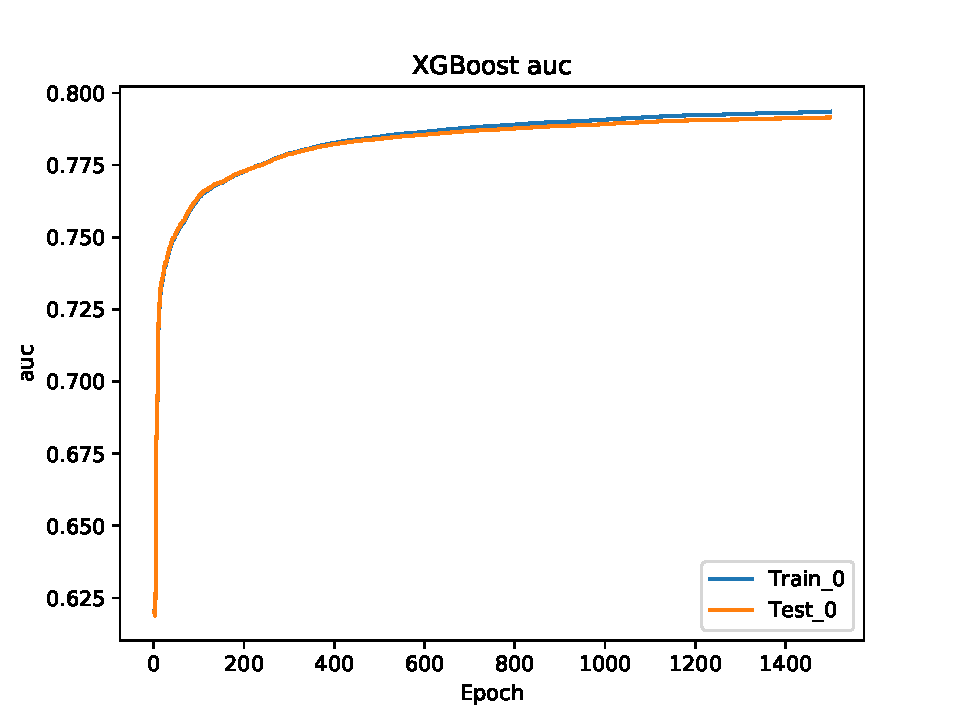
\includegraphics[width=.9\linewidth]{Appendices/BDT/Evolutionplots/auc_OS_ttbar_K0}
  \caption{Area under the ROC curve.}
  \label{fig:ChaptH:EventSelection:BDT:Epochs:ttbarOS:AUC}
\end{subfigure}%
\begin{subfigure}{.475\textwidth}
  \centering
  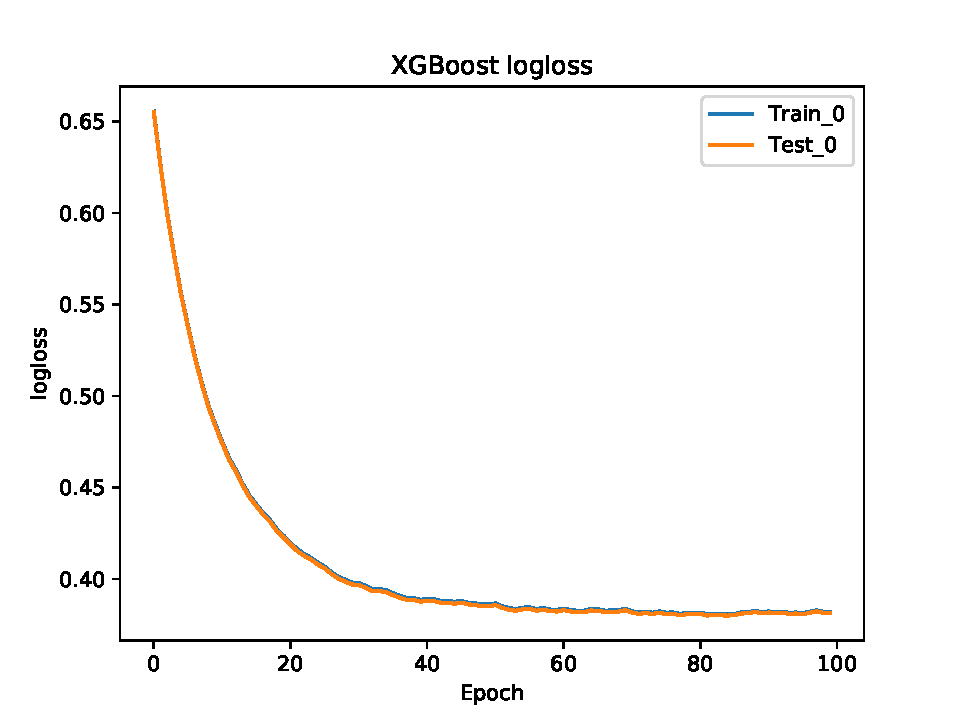
\includegraphics[width=.9\linewidth]{Appendices/BDT/Evolutionplots/logloss_OS_ttbar_K0}
  \caption{Logarithm of the loss function.}
  \label{fig:ChaptH:EventSelection:BDT:Epochs:ttbarOS:LogLoss}
\end{subfigure}
\caption{Evolution of the AUC and LogLoss functions for the training of the BDT$(\ttbar|_{\text{OS}})$.
The x-axis shows the training iteration.}
\label{fig:ChaptH:EventSelection:BDT:Epochs:ttbarOS}
\end{figure}

\begin{figure}[h]
\centering
\begin{subfigure}{.475\textwidth}
  \centering
  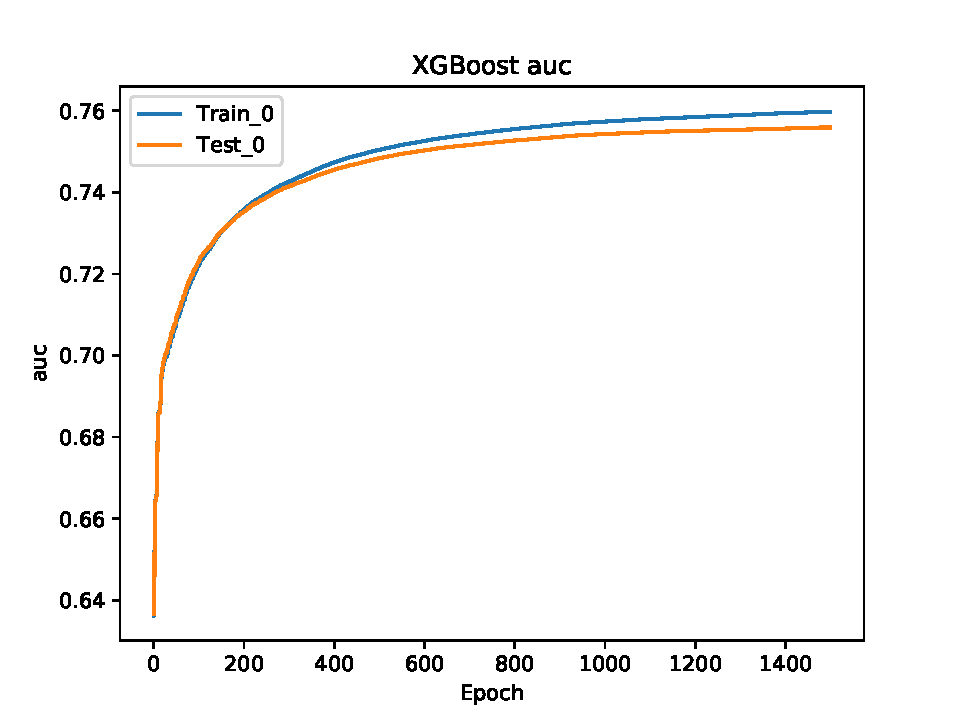
\includegraphics[width=.9\linewidth]{Appendices/BDT/Evolutionplots/auc_SS_tHq_K0}
  \caption{Area under the ROC curve.}
  \label{fig:ChaptH:EventSelection:BDT:Epochs:tHqSS:AUC}
\end{subfigure}%
\begin{subfigure}{.475\textwidth}
  \centering
  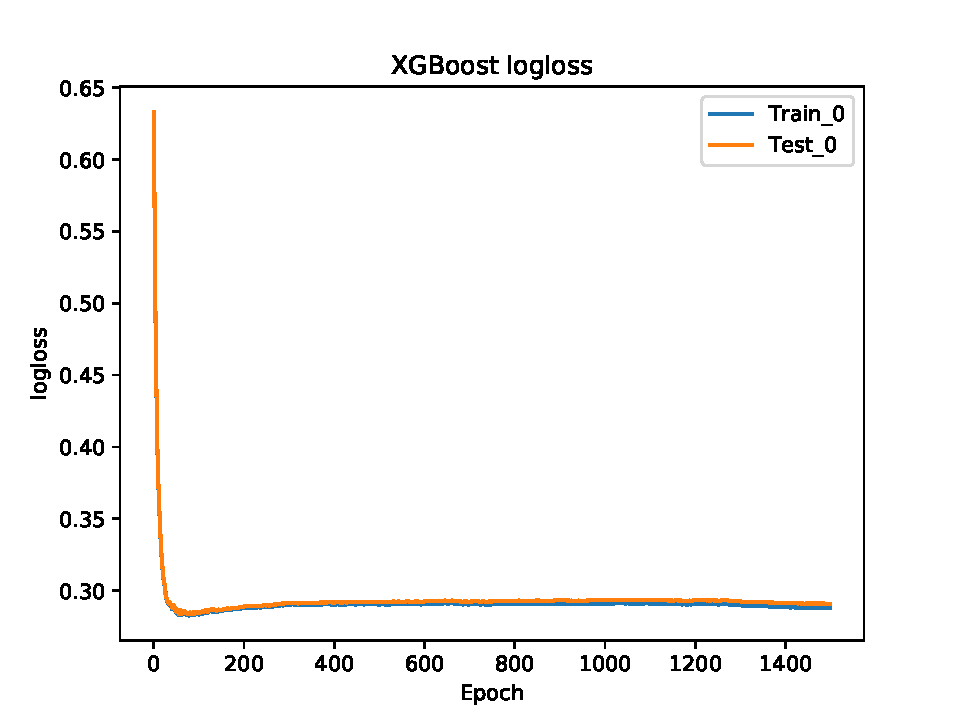
\includegraphics[width=.9\linewidth]{Appendices/BDT/Evolutionplots/logloss_SS_tHq_K0}
  \caption{Logarithm of the loss function.}
  \label{fig:ChaptH:EventSelection:BDT:Epochs:tHqSS:LogLoss}
\end{subfigure}
\caption{Evolution of the AUC and LogLoss functions for the training of the BDT$(\tHq|_{\text{SS}})$.
The x-axis shows the training iteration.}
\label{fig:ChaptH:EventSelection:BDT:Epochs:tHqSS}
\end{figure}

\begin{comment}
\begin{table}[]
\centering
\begin{tabular}{|l|l|l|l|l|}
\toprule
Region       			& \tHq & Total & \StoB (\%) & Significance \\ \midrule
Preselection 			& 1.2 & 130.1 & 0.93    & 0.106             \\
BDT$(\tHq) \geq$0.05       & 1.2 & 130.1 & 0.93    & 0.106             \\
BDT$(\tHq) \geq$0.10       & 1.2 & 130.1 & 0.93    & 0.106             \\
BDT$(\tHq) \geq$0.15       & 1.2 & 128.9 & 0.94    & 0.106             \\
BDT$(\tHq) \geq$0.20       & 1.2 & 123.9 & 0.98    & 0.108             \\
BDT$(\tHq) \geq$0.25       & 1.2 & 115.9 & 1.05    & 0.112             \\
BDT$(\tHq) \geq$0.30       & 1.2 & 105.7 & 1.15    & 0.117             \\
BDT$(\tHq) \geq$0.35       & 1.2 & 94.5  & 1.29    & 0.124             \\
BDT$(\tHq) \geq$0.40       & 1.1 & 82.8  & 1.35    & 0.121             \\
BDT$(\tHq) \geq$0.45       & 1.1 & 70.4  & 1.59    & 0.132             \\
BDT$(\tHq) \geq$0.50       & 1.1 & 59.6  & 1.88    & 0.143             \\
BDT$(\tHq) \geq$0.55       & 1.0 & 49.8  & 2.05    & 0.143             \\
BDT$(\tHq) \geq$0.60       & 1.0 & 40.3  & 2.54    & 0.159             \\
BDT$(\tHq) \geq$0.65       & 0.9 & 31.2  & 2.97    & 0.163             \\
BDT$(\tHq) \geq$0.70       & 0.8 & 23.4  & 3.54    & 0.167             \\
BDT$(\tHq) \geq$0.75       & 0.7 & 16.4  & 4.46    & 0.175             \\
BDT$(\tHq) \geq$0.80       & 0.6 & 10.9  & 5.83    & 0.185             \\
BDT$(\tHq) \geq$0.85       & 0.4 & 5.1   & 8.51    & 0.182             \\
BDT$(\tHq) \geq$0.90       & 0.2 & 1.8   & 12.50   & 0.155             \\
BDT$(\tHq) \geq$0.95       & 0.0 & 0.0   & 0.00    & 0.000            \\ \bottomrule
\end{tabular}
\caption{Signal to background ratio and significance of the \tHq signal in the \dilepSStau channel
depending on the cut applied on the BDT(\tHq - \dilepSStau) score distribution. \pablo{Esto se puede convertir en una gràfica}}
\label{tab:ChaptH:EventSelection:SR:SS:BDT_score_distribution}
\end{table}




\pablo{Poner el escaneo de valores de cortes en \HT en forma de plot}
\begin{table}[]
\centering
\begin{tabular}{l|l|l|l|l}
\toprule
BDT$(\tHq)<$ 0.65 + & \multirow{2}{*}{\ttX} & \multirow{2}{*}{Total} & \multirow{2}{*}{$\frac{\ttX}{Total}$ (\%)} & \multirow{2}{*}{Significance} \\
\HT [GeV] cut      &                      &                        &                                &                               \\ \midrule
$\HT >$250 & 59.9 & 80.5 & 74.41 & 9.98 \\
$\HT >$255 & 58.7 & 78.8 & 74.49 & 9.90 \\
$\HT >$260 & 57.4 & 77.3 & 74.26 & 9.75 \\
$\HT >$265 & 56.5 & 75.7 & 74.64 & 9.73 \\
$\HT >$270 & 55.2 & 73.6 & 75.00 & 9.68 \\
$\HT >$275 & 53.8 & 71.8 & 74.93 & 9.54 \\
$\HT >$280 & 52.7 & 70.3 & 74.96 & 9.45 \\
$\HT >$285 & 51.4 & 68.5 & 75.04 & 9.34 \\
$\HT >$290 & 50.1 & 66.6 & 75.23 & 9.26 \\
$\HT >$295 & 48.8 & 64.5 & 75.66 & 9.20 \\
$\HT >$300 & 47.5 & 62.9 & 75.52 & 9.06 \\ \bottomrule
\end{tabular}
\caption{ Concentration of the \ttX processes as a function of the minimum \HT required in the region of the phase space orthogonal to \dilepSStau SR.
This is used to define the CR(\ttX). \pablo{quitar tabla}}
\label{tab:tHq:EventSelection:CR:SS:HTScan_ttX}
\end{table}




\begin{table}[]
\centering
\begin{tabular}{l|l|l|l|l|l|l|l}
\toprule
BDT(\tHq) < 0.65 + & \multirow{2}{*}{\ttX} & \multirow{2}{*}{\ttW} & \multirow{2}{*}{\ttZ} & \multirow{2}{*}{\ttH} & \multirow{2}{*}{Total} & \multirow{2}{*}{$\frac{\ttX}{Total}$ (\%)} & \multirow{2}{*}{Significance} \\
 \HT [GeV] cut                 &                      &                      &                      &                      &                        &                                &                               \\ \midrule
 $ \HT >$250 & 59.9 & 27.1 & 14.7 & 18.1 & 80.5 & 74.41 & 9.982 \\
 $ \HT >$255 & 58.7 & 26.5 & 14.5 & 17.7 & 78.8 & 74.49 & 9.895 \\
 $ \HT >$260 & 57.4 & 26.0 & 14.0 & 17.4 & 77.3 & 74.26 & 9.746 \\
 $ \HT >$265 & 56.5 & 25.5 & 14.0 & 17.0 & 75.7 & 74.64 & 9.731 \\
 $ \HT >$270 & 55.2 & 24.9 & 13.7 & 16.6 & 73.6 & 75.00 & 9.678 \\
 $ \HT >$275 & 53.8 & 24.3 & 13.4 & 16.1 & 71.8 & 74.93 & 9.543 \\
 $ \HT >$280 & 52.7 & 23.8 & 13.1 & 15.8 & 70.3 & 74.96 & 9.451 \\
 $ \HT >$285 & 51.4 & 23.2 & 12.8 & 15.4 & 68.5 & 75.04 & 9.345 \\
 $ \HT >$290 & 50.1 & 22.6 & 12.6 & 14.9 & 66.6 & 75.23 & 9.255 \\
 $ \HT >$295 & 48.8 & 22.1 & 12.2 & 14.5 & 64.5 & 75.66 & 9.202 \\
 $ \HT >$300 & 47.5 & 21.6 & 11.8 & 14.1 & 62.9 & 75.52 & 9.057            \\ \bottomrule            

\end{tabular}
\caption{Scanning the abundance of the \ttX process depending on the minimum \HT required in the region of 
the phase space orthogonal to \dilepSStau SR. This is used to define the CR(\ttX). This table also 
presents the yields of the \ttW, \ttZ, and \ttH processes, showing that \ttW is the dominant among them.}
\label{tab:tHq:EventSelection:CR:SS:HTScan_ttX_b}
\end{table}


\begin{table}[]
\centering
\begin{tabular}{l|l|l|l|l}
\toprule
BDT$(\tHq)<$ 0.6 + & \multirow{2}{*}{\ttbar} 	& \multirow{2}{*}{Total} & \multirow{2}{*}{$\frac{\ttbar}{Total}$ (\%)} & \multirow{2}{*}{Significance} \\
\HT [GeV] cut           &                      			&                                  &                                				     &                               \\ \midrule
$ \HT \leq $245 & 6.9 & 19.1 & 36.13 & 1.823 \\
$ \HT \leq $250 & 7.4 & 20.8 & 35.58 & 1.869 \\
$ \HT \leq $255 & 7.9 & 22.5 & 35.11 & 1.914 \\
$ \HT \leq $260 & 8.1 & 24.0 & 33.75 & 1.888 \\
$ \HT \leq $265 & 8.3 & 25.6 & 32.42 & 1.861 \\
$ \HT \leq $270 & 8.8 & 27.6 & 31.88 & 1.896 \\
$ \HT \leq $275 & 9.1 & 29.5 & 30.85 & 1.887 \\
$ \HT \leq $280 & 9.3 & 31.0 & 30.00 & 1.875 \\
$ \HT \leq $285 & 9.6 & 32.8 & 29.27 & 1.875 \\ \bottomrule
\end{tabular}
\caption{Scanning purity of the \ttbar process depending requirement on the maximum \HT allowed 
in the region of the phase space orthogonal to \dilepSStau SR.
This is used to define the CR(\ttbar).}
\label{tab:tHq:EventSelection:CR:SS:HTScan_ttbar}
\end{table}

\end{comment}


\begin{comment}
\FloatBarrier
%%%%%%%%%%%%%%%%%%
%             Additional models           %
%%%%%%%%%%%%%%%%%%
\section{Alternative BDT-based Models}
\label{sec:BDT:AltModels}
In this section, I present some of the most relevant BDT-based models that were trained but not ultimately used in the final analysis of this PhD thesis. These models were developed as alternative approaches to tackle specific aspects of the analysis or to explore different signal and background processes. Although they were not included in the final analysis, they provide valuable insights and potential avenues for future research.

%% Assignment
\subsection{Alternative model for lepton assignment in the \dilepSStau channnel}
\label{sec:BDT:AltModels:Assignment}
Apart from the $\text{BDT}^{\text{Lepton Assignment}}$ used for the light-lepton assignment algorithm
described in Section~\ref{sec:ChaptH:Sig:LepAsign}, other ML-based approaches were explored
as well.  
Within the gradient BDTs, different configurations are explored regarding the number of folds, the hyperparameters
and the collection of input variables. Several of these offer a similar performance to the chosen $\text{BDT}^{\text{Lepton Assignment}}$.
Besides the BDTs, other algorithms such as NN and random forests~\cite{ho1995random} have been teste and, although they showed
promising performances, none of them are adopted in the final analysis.

%One of the BDT-based models developed during this study focused on improving the lepton assignment algorithm. 
%The lepton assignment plays a crucial role in reconstructing the final state particles in many physics analyses. 
%The alternative BDT model was trained to optimise the assignment of leptons in the event, taking into account 
% their kinematic properties, isolation, and other relevant observables.
%Although this model showed promising performance in preliminary studies, it was not ultimately adopted in the final 
%analysis due to the need for further validation and a through assessment of its impact on the analysis outcomes.


%% Zjets OS
\subsection{BDT$(\PZ+\text{jets}|_{\text{OS}})$}
\label{sec:BDT:AltModels:ZjetsOS}
The production of \PZ bosons in association with jets (\Zjets) is, along with \ttbar, the most important background process for the \dilepOStau. 
To better discriminate between the \Zjets background, %and the signal process of interest, 
a dedicated BDT model was trained. 

However, further investigations revealed that the BDT model targeting \ttbar is achieving the same
same as the BDT for \Zjets, which was to separate these two processes. Therefore, the decision was 
made to use only the BDT$(\ttbar|_{\text{OS}})$, as it already effectively accounted for the separation from the \Zjets and \ttbar.

The capabilities of the BDT$(\ttbar|_{\text{OS}})$ are very similar to the model that targeted \Zjets, BDT$(\Zjets|_{\text{OS}})$.
This model is presented here through its features (Figure~\ref{fig:BDT:AltModels:ZjetsOS:Vars}) and hyperparameters 
(Table~\ref{tab:BDT:AltModels:ZjetsOS:hyper}). 
Not surprisingly, the \MET ranks the highest. It is presented in Figure~\ref{fig:Appendix:BDTVARS:ttbarOS:a02_PR_MET} of
 Appendix~\ref{chap:Appendix:BDT_Variables}. This variable is very efficient separating the \Zjets and \ttbar production in
the \dilepOStau final state because there are fewer final-state neutrinos for the \Zjets.
While this model is not used, its ability to discriminate is more than acceptable
as it can be seen trough its ROC (Figure~\ref{fig:BDT:AltModels:ZjetsOS:ROC}) and its score distribution 
(Figure~\ref{fig:BDT:AltModels:ZjetsOS:Score}). 

%\begin{figure}[ht!]
%    \centering
    \begin{minipage}[c]{0.55\textwidth}
    %\begin{figure}[h]
        %\centering
        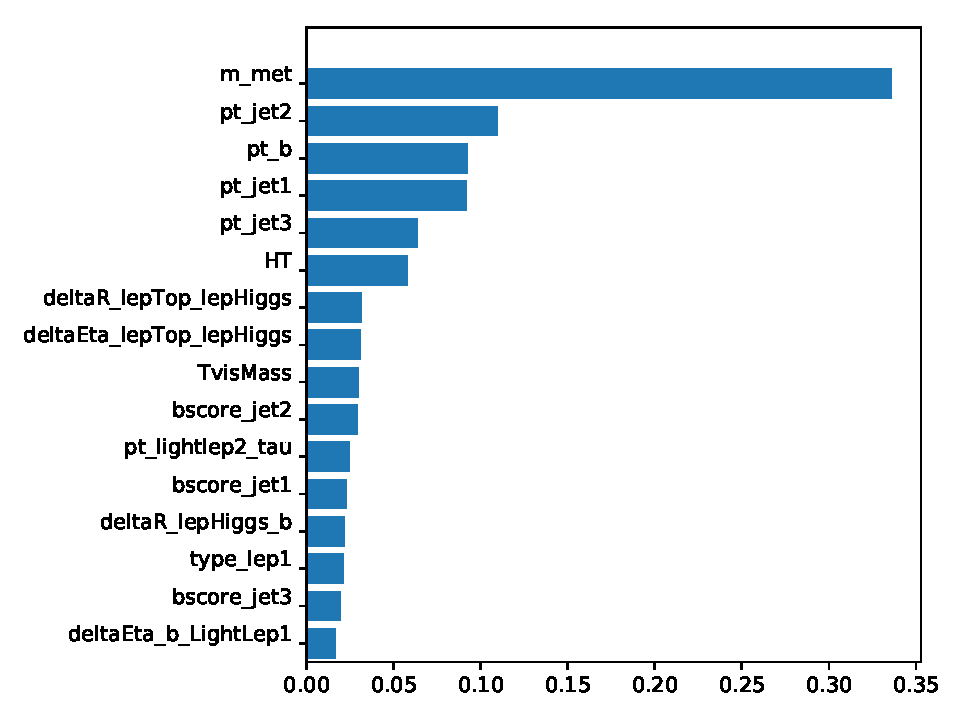
\includegraphics[width=\textwidth]{Appendices/BDT/AlternativeModels/OS_Zjets/Feature_importance_Zjets_OS} 
        \captionof{figure}{Ranking of input variables for BDT$(\Zjets|_{\text{OS}})$}
        \label{fig:BDT:AltModels:ZjetsOS:Vars}
        %\end{figure}
    \end{minipage}
    \hfill
    \begin{minipage}{0.4\textwidth}
	\centering
	\begin{adjustbox}{max width=0.99\textwidth}
		\begin{tabular}{l|c}
		\toprule
		Hyperparameter            	& BDT$(\tWH|_{\text{OS}})$ \\ \midrule
		Maximum depth             	& 5                        \\
		Learning rate             	& 0.05                   \\
		Number of estimators      	& 2500                     \\
		Minimum child weight       	& 0.7                     \\
		Scale of positive weights 	& 12                  \\
		Neg. weight strategy      	& Pos. only           \\ \bottomrule
		\end{tabular}
	\end{adjustbox}
	\captionof{table}{Hyperparameters controlling the training of the BDT$(\Zjets|_{\text{OS}})$.}
	\label{tab:BDT:AltModels:ZjetsOS:hyper}
    \end{minipage}
%\end{figure}

\begin{figure}[h]
\centering
\begin{subfigure}{.475\textwidth}
  \centering
  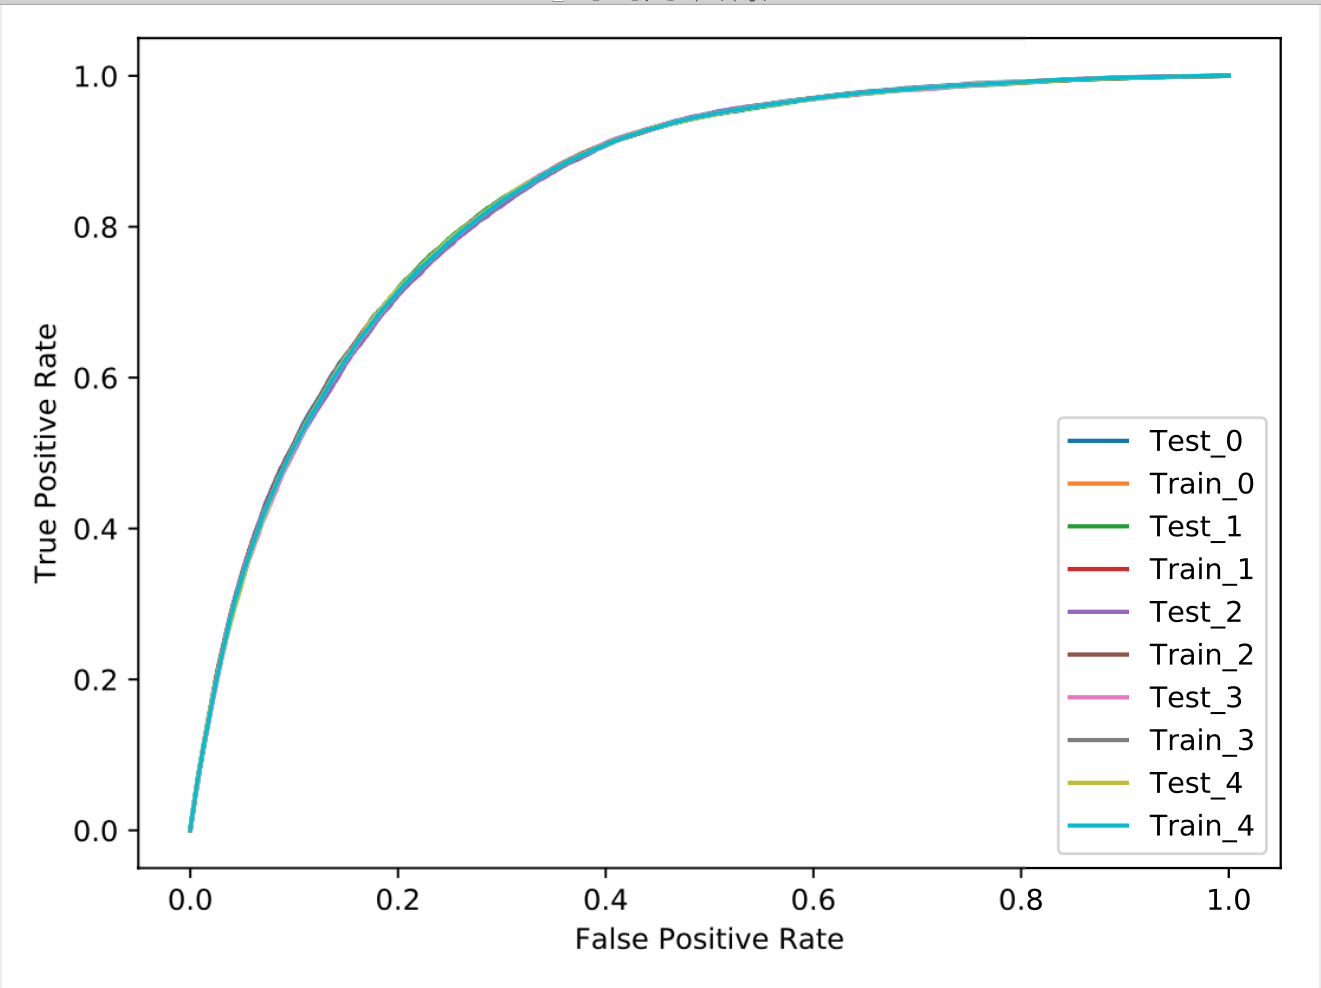
\includegraphics[width=.9\linewidth]{Appendices/BDT/AlternativeModels/OS_Zjets/Roc_curve_Zjets_OS_LowRes}
  \caption{ROC}
  \label{fig:BDT:AltModels:ZjetsOS:ROC}
\end{subfigure}%
\begin{subfigure}{.5\textwidth}
  \centering
  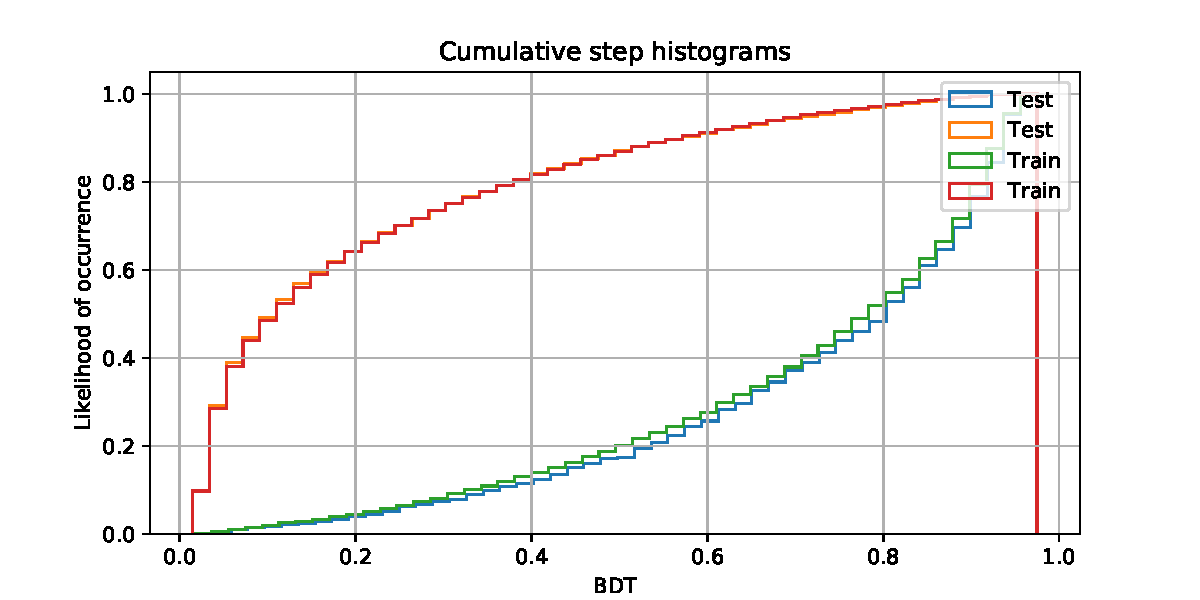
\includegraphics[width=.99\linewidth]{Appendices/BDT/AlternativeModels/OS_Zjets/BDT_cumulative_response_Zjets_K1_OS}
  \caption{Cumulative distribution}
  \label{fig:BDT:AltModels:ZjetsOS:Score}
\end{subfigure}
\caption{ROC and cumulative distribution of the BDT$(\Zjets|_{\text{OS}})$.
The \Zjets production is presented in green (train) and blue (test), and the score for the rest of the processes
is presented in red (train) and orange (test).}
\label{fig:BDT:AltModels:Result:ZjetsOS}
\end{figure}



%% tWH OS
\subsection{BDT$(\tWH|_{\text{OS}})$}
\label{sec:BDT:AltModels:tWHOS}
In order to comprehensively test the hypothesis $\yt = -1$, it is essential to consider not only the \tHq production process but also the \tWH process. To perform a combined fit where the entire \tH production is treated as a signal, it is important to have a BDT model that can effectively identify the \tWH process to fit it alongside \tHq.

The first practical approach consists of creating separate BDT models for each process rather than to have a single 
BDT model that targets both processes simultaneously. While it may seem intuitive to train a single BDT model targeting both processes, 
such an approach can be challenging due to the inherent differences between \tHq and \tWH events. 
Creating individual BDT models, one for \tHq and another for \tWH, allows for a more focused and optimised training process. 
Each model can be tailored to the specific characteristics and kinematic properties of its respective process, resulting in improved 
performance and discrimination power.

The training of the model targeting the \tWH process in the \dilepOStau channel is presented through the 
selection of its features in Figure~\ref{fig:BDT:AltModels:tWHOS:Vars} and its hyperparameters
in Table~\ref{tab:BDT:AltModels:tWHOS:hyper}. The evolution of the training is shown via
its AUC and LogLoss in Figures~\ref{fig:BDT:AltModels:tWHOS:AUC} and~\ref{fig:BDT:AltModels:tWHOS:LogLoss}.
The divergence in the train a test curves in the AUC evolution plot is a symptom of overtraining. 
Figure~\ref{fig:BDT:AltModels:tWHOS:ROC} shows the ROC curves for all folds of the model.
In this figure, it can be seen that the ROC is not identical for all folds. 
The capability of the model to separate \tWH from the rest of the precesses is best described by
Figure~\ref{fig:BDT:AltModels:tWHOS:Score}, where it can be seen that by performing a but
in BDT$(\tWH|_{\text{OS}})=0.2$, less than 30\% of \tWH is lost and more than 80\% of
the other processes can be removed. 

Since the scope of this thesis is limited to the study of the \tHq production, the trained BDT$(\tWH|_{\text{OS}}$)
model has not been implemented but it can be used in the ongoing ATLAS analysis in order to search
for the more inclusive \tH production. 

%\begin{figure}[h]
%    \centering
    \begin{minipage}{0.55\textwidth}
        \centering
        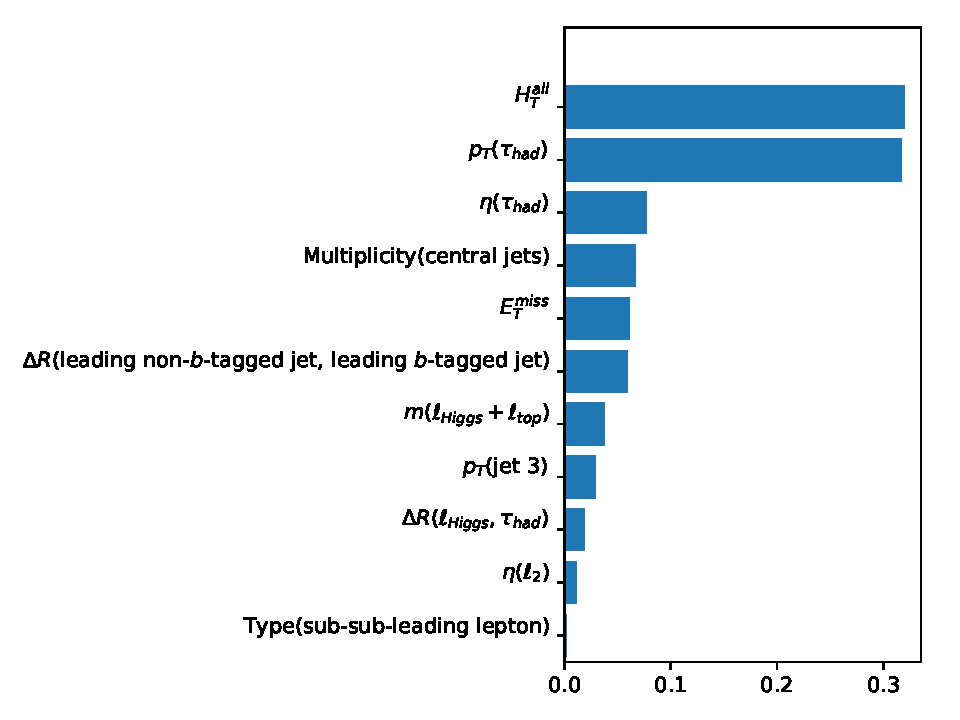
\includegraphics[width=\textwidth]{Appendices/BDT/AlternativeModels/OS_tWH/Feature_importance_tWH_OS_test} 
        \captionof{figure}{Ranking of input variables for BDT$(\tWH|_{\text{OS}})$}
        \label{fig:BDT:AltModels:tWHOS:Vars}
    \end{minipage}
    \hfill
    \begin{minipage}{0.4\textwidth}
	\centering
	\begin{adjustbox}{max width=0.99\textwidth}
		\begin{tabular}{l|c}
		\toprule
		Hyperparameter            	& BDT$(\tWH|_{\text{OS}})$ \\ \midrule
		Maximum depth             	& 4                        \\
		Learning rate             	& 0.15                   \\
		Number of estimators      	& 1000                     \\
		Minimum child weight       	& 1.3                     \\
		Scale of positive weights 	& 400                  \\
		Neg. weight strategy      	& All events           \\ \bottomrule
		\end{tabular}
	\end{adjustbox}
	\captionof{table}{Hyperparameters controlling the training of the BDT$(\tWH|_{\text{OS}})$.}
	\label{tab:BDT:AltModels:tWHOS:hyper}
    \end{minipage}
%\end{figure}

\begin{figure}[h]
\centering
\begin{subfigure}{.475\textwidth}
  \centering
  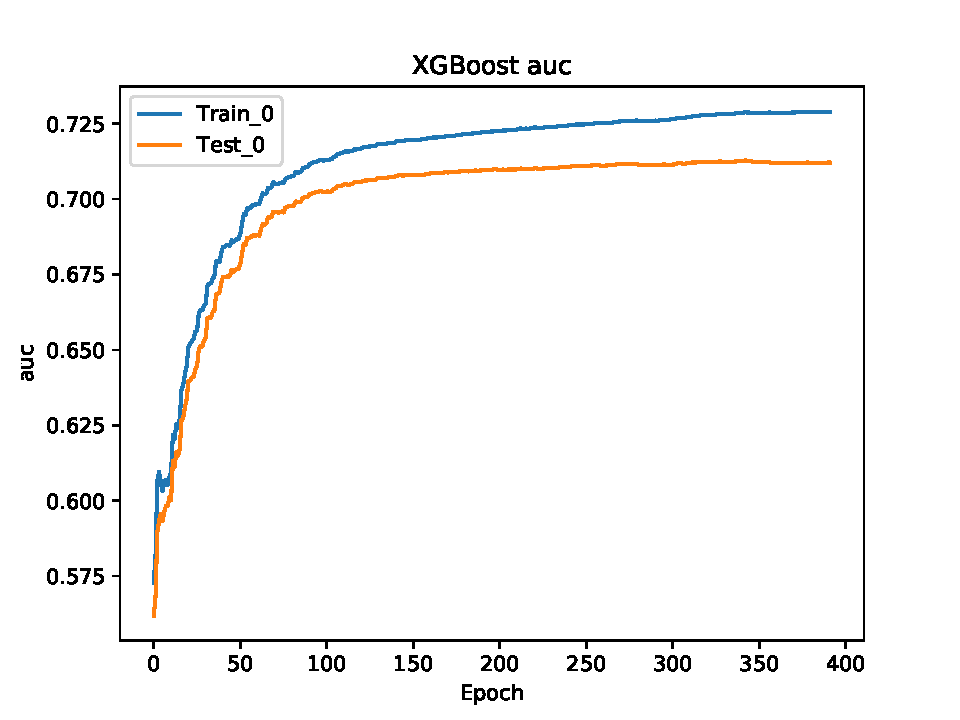
\includegraphics[width=.9\linewidth]{Appendices/BDT/AlternativeModels/OS_tWH/auc_tWH_K3_OS_test}
  \caption{Area under the ROC curve.}
  \label{fig:BDT:AltModels:tWHOS:AUC}
\end{subfigure}%
\begin{subfigure}{.475\textwidth}
  \centering
  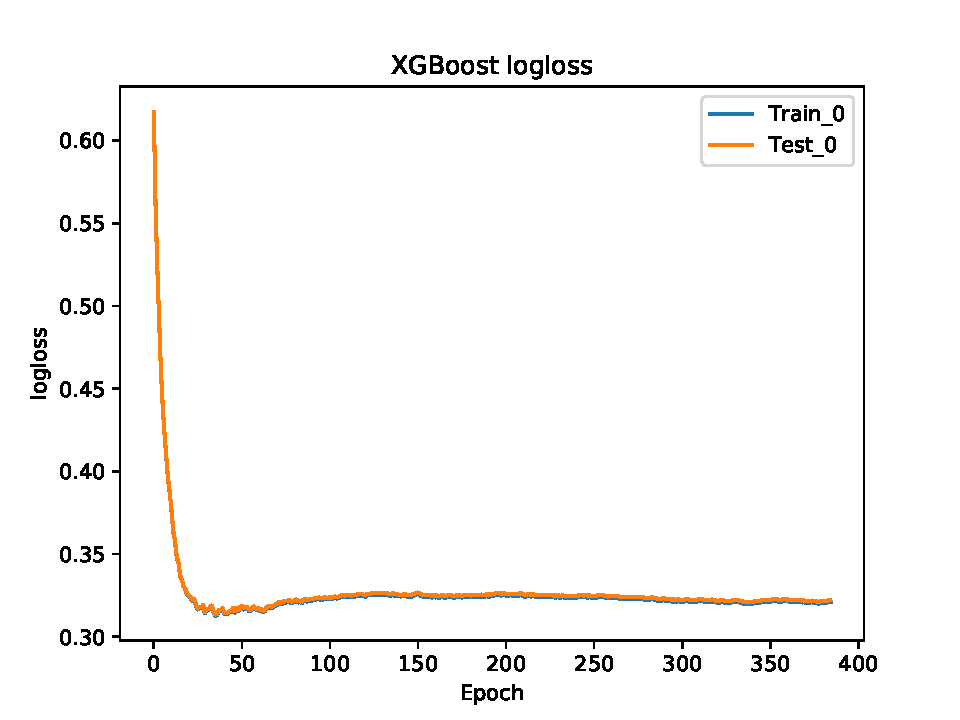
\includegraphics[width=.9\linewidth]{Appendices/BDT/AlternativeModels/OS_tWH/logloss_tWH_K2_OS_test}
  \caption{Logarithm of the loss function.}
  \label{fig:BDT:AltModels:tWHOS:LogLoss}
\end{subfigure}
\caption{Evolution of the AUC and LogLoss functions for the training of the BDT$(\tWH|_{\text{OS}})$.
As the training progress, in the AUC plot can be observed a separation between the distributions for the 
train and test. While it can look like overtraining, note that the difference in train and test is less than 4\%.}
\label{fig:BDT:AltModels:Epochs:tWHOS}
\end{figure}


\begin{figure}[h]
\centering
\begin{subfigure}{.475\textwidth}
  \centering
  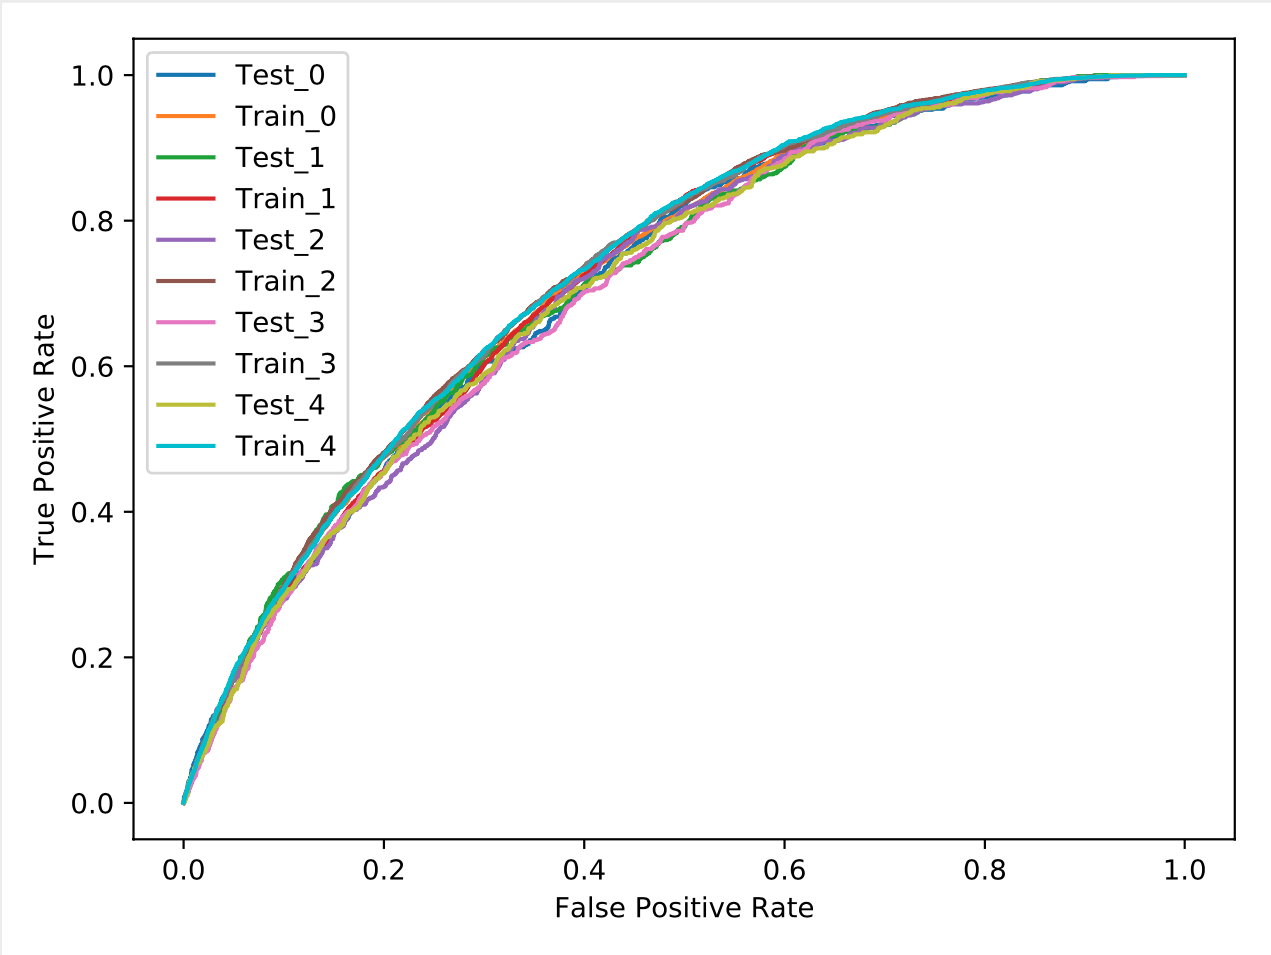
\includegraphics[width=.9\linewidth]{Appendices/BDT/AlternativeModels/OS_tWH/Roc_curve_tWH_OS_test_LowRes}
  \caption{ROC}
  \label{fig:BDT:AltModels:tWHOS:ROC}
\end{subfigure}%
\begin{subfigure}{.5\textwidth}
  \centering
  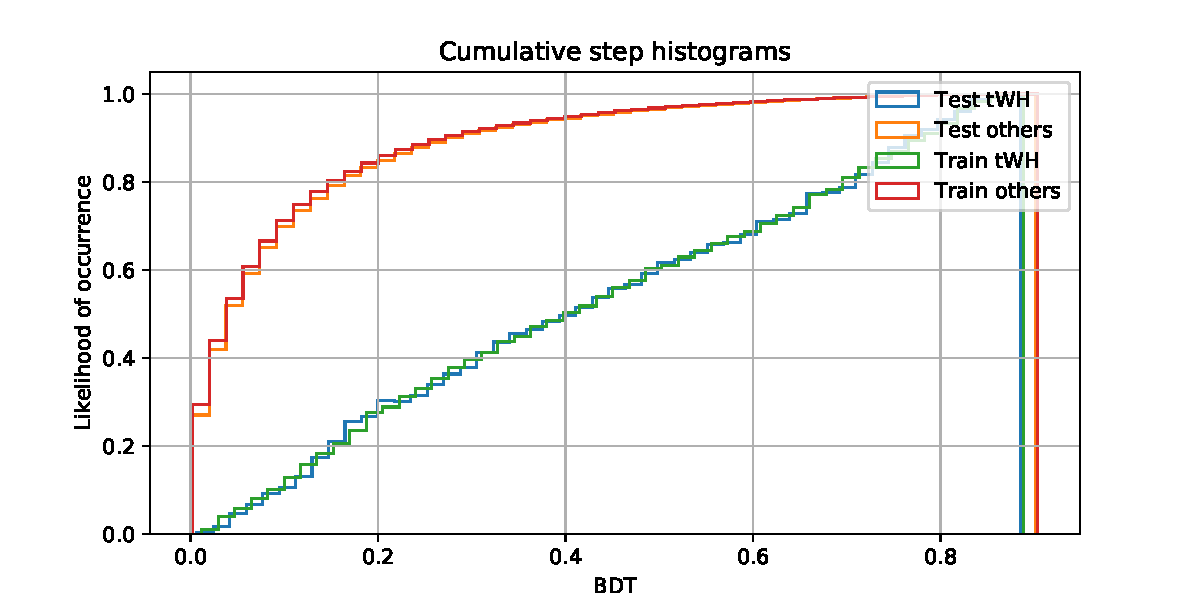
\includegraphics[width=.99\linewidth]{Appendices/BDT/AlternativeModels/OS_tWH/BDT_cumulative_response_tWH_K3_OS_test}
  \caption{Cumulative distribution}
  \label{fig:BDT:AltModels:tWHOS:Score}
\end{subfigure}
\caption{ROC and cumulative distribution of the BDT$(\tWH|_{\text{OS}})$.}
\label{fig:BDT:AltModels:Result:tWHOS}
\end{figure}

%\subsection{BDT$(\tWH|_{\text{SS}})$}
%\label{sec:BDT:AltModels:tWHSS}
%In agreement with the idea presented in the Section~\ref{sec:BDT:AltModels:tWHOS}, a BDT
%for the \tHW in the \dilepSStau channel is trained as well. Nevertheless, due to the scarcity of
%data in this region of the phase space, the training of such model was quite inestable. 

%\subsection{BDT$(\ttbar|_{\text{SS}})$}
%\label{sec:BDT:AltModels:ttbarSS}

%% ttW SS
\subsection{BDT$(\ttW|_{\text{SS}})$}
\label{sec:BDT:AltModels:ttWSS}
As seen in Section~\ref{sec:ChaptH:EventSelection:CR:SS}, separating the \ttW background from the rest 
of the processes in the \dilepSStau channel is quite challenging. Nevertheless, it has been attempted and
a model trying to fulfil this task is discussed in this section. In Figure~\ref{fig:BDT:AltModels:ttWSS:Vars} and 
Table~\ref{tab:BDT:AltModels:ttWSS:hyper} the features and hyperparameters used in the training of the 
BDT$(\ttW|_{\text{SS}})$ are presented.  In both curves of Figure~\ref{fig:BDT:AltModels:Epochs:ttWSS}
can be observed that the training of the BDT$(\ttW|_{\text{SS}})$ is stopped before the AUC or the
LogLoss has reached a plateau, suggesting that further training could improve the accuracy of
the model. The ROCs of all five folds are presented simultaneously in Figure~\ref{fig:BDT:AltModels:ttWSS:ROC}.
While all the folds present the same profile, this is relatively close to a straight line that would indicate random
guessing. The lack of discriminating ability of the model is further checked in the cumulative distribution plot (Figure~\ref{fig:BDT:AltModels:ttWSS:Score} ), 
in which the curve of the \ttW process is very close to the curve of the other processes. For instance,
in Figure~\ref{fig:BDT:AltModels:ttWSS:Score} can be seen that a cut around BDT$(\ttW|_{\text{SS}})=0.5$
would remove less than 40\% of all \tWH events and more than 70\% of the rest of the processes. 
This is a bad separation when compared to the other BDTs such as BDT$(\ttbar|_{\text{OS}})$, where
it is possible to remove 80\% of the other process while losing only 7\% of \ttbar.


%\begin{figure}[h]
 %   \centering
    \begin{minipage}{0.55\textwidth}
        \centering
        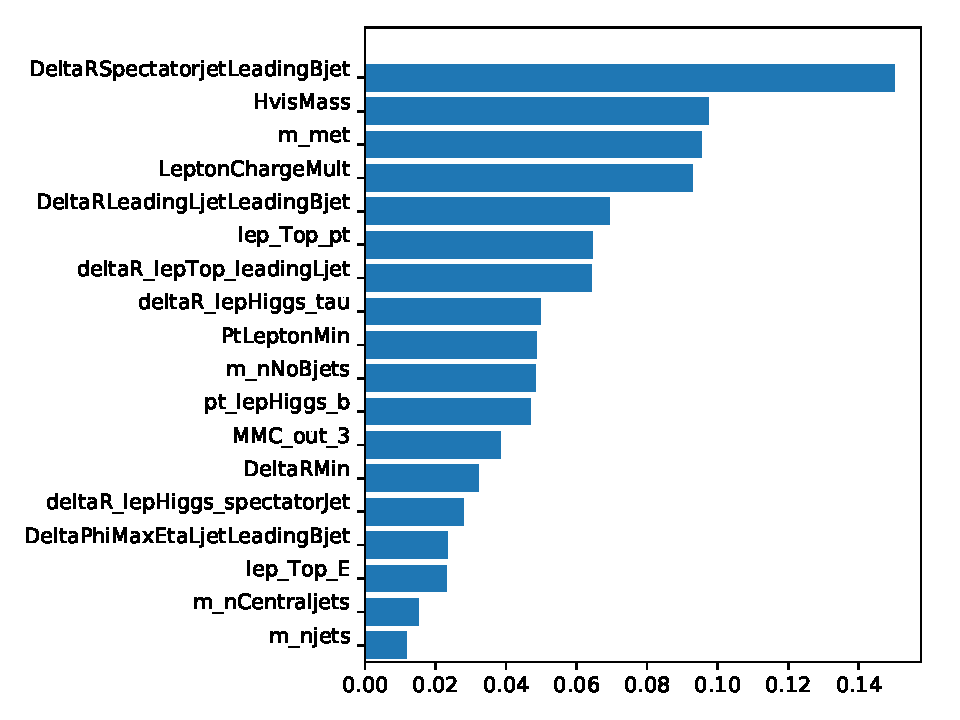
\includegraphics[width=\textwidth]{Appendices/BDT/AlternativeModels/SS_ttW/Feature_importance_ttW_SS_test}
        \captionof{figure}{Ranking of input variables for BDT$(\ttW|_{\text{SS}})$}
        \label{fig:BDT:AltModels:ttWSS:Vars}
    \end{minipage}
    \hfill
    \begin{minipage}{0.4\textwidth}
	\centering
	\begin{adjustbox}{max width=0.99\textwidth}
		\begin{tabular}{l|c}
		\toprule
		Hyperparameter            	& BDT$(\ttW|_{\text{SS}})$ \\ \midrule
		Maximum depth             	& 4                        \\
		Learning rate             	& 0.03                   \\
		Number of estimators      	& 1500                     \\
		Minimum child weight       	& 0.05                     \\
		Scale of positive weights 	& 4                  \\
		Neg. weight strategy      	& All events           \\ \bottomrule
		\end{tabular}
	\end{adjustbox}
	\captionof{table}{Hyperparameters controlling the training of the BDT$(\ttW|_{\text{SS}})$.}
	\label{tab:BDT:AltModels:ttWSS:hyper}
    \end{minipage}
%\end{figure}

\begin{figure}[h]
\centering
\begin{subfigure}{.475\textwidth}
  \centering
  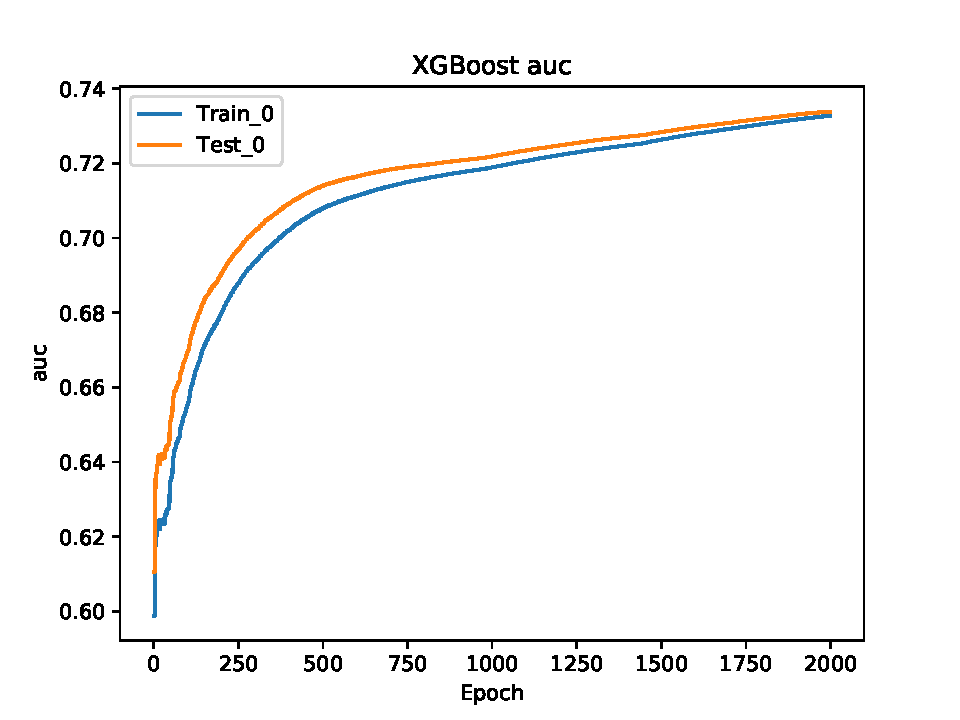
\includegraphics[width=.9\linewidth]{Appendices/BDT/AlternativeModels/SS_ttW/auc_ttW_K2_SS_test}
  \caption{Area under the ROC curve.}
  \label{fig:BDT:AltModels:ttWSS:AUC}
\end{subfigure}%
\begin{subfigure}{.475\textwidth}
  \centering
  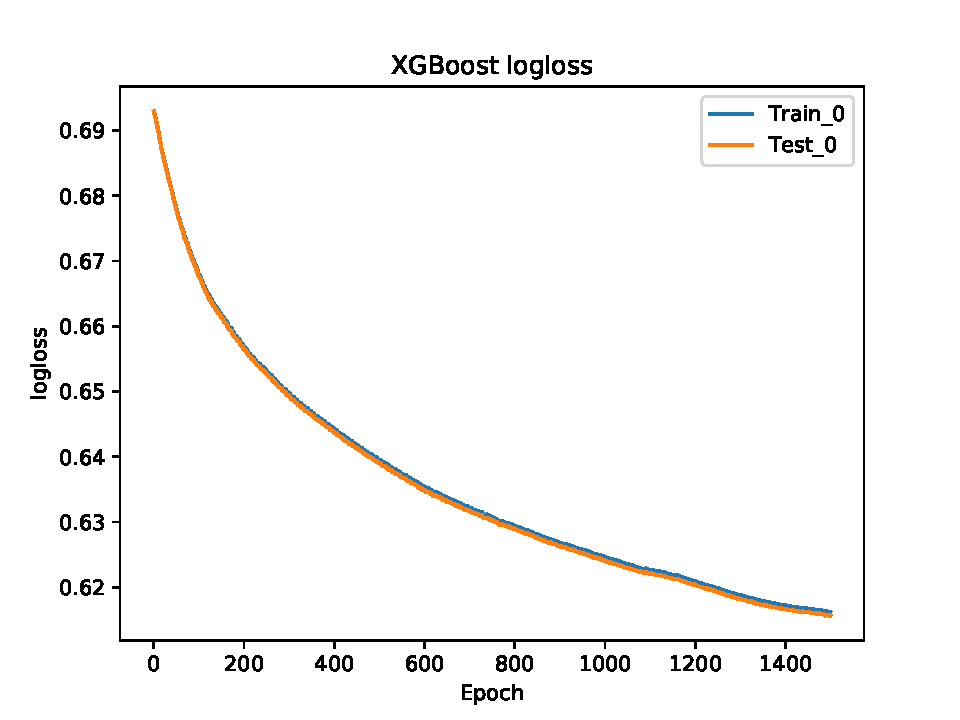
\includegraphics[width=.9\linewidth]{Appendices/BDT/AlternativeModels/SS_ttW/logloss_ttW_K2_SS_LR_003}
  \caption{Logarithm of the loss function.}
  \label{fig:BDT:AltModels:ttWSS:LogLoss}
\end{subfigure}
\caption{Evolution of the AUC and LogLoss functions for the training of the BDT$(\ttW|_{\text{SS}})$.}
\label{fig:BDT:AltModels:Epochs:ttWSS}
\end{figure}

\begin{figure}[h]
\centering
\begin{subfigure}{.475\textwidth}
  \centering
  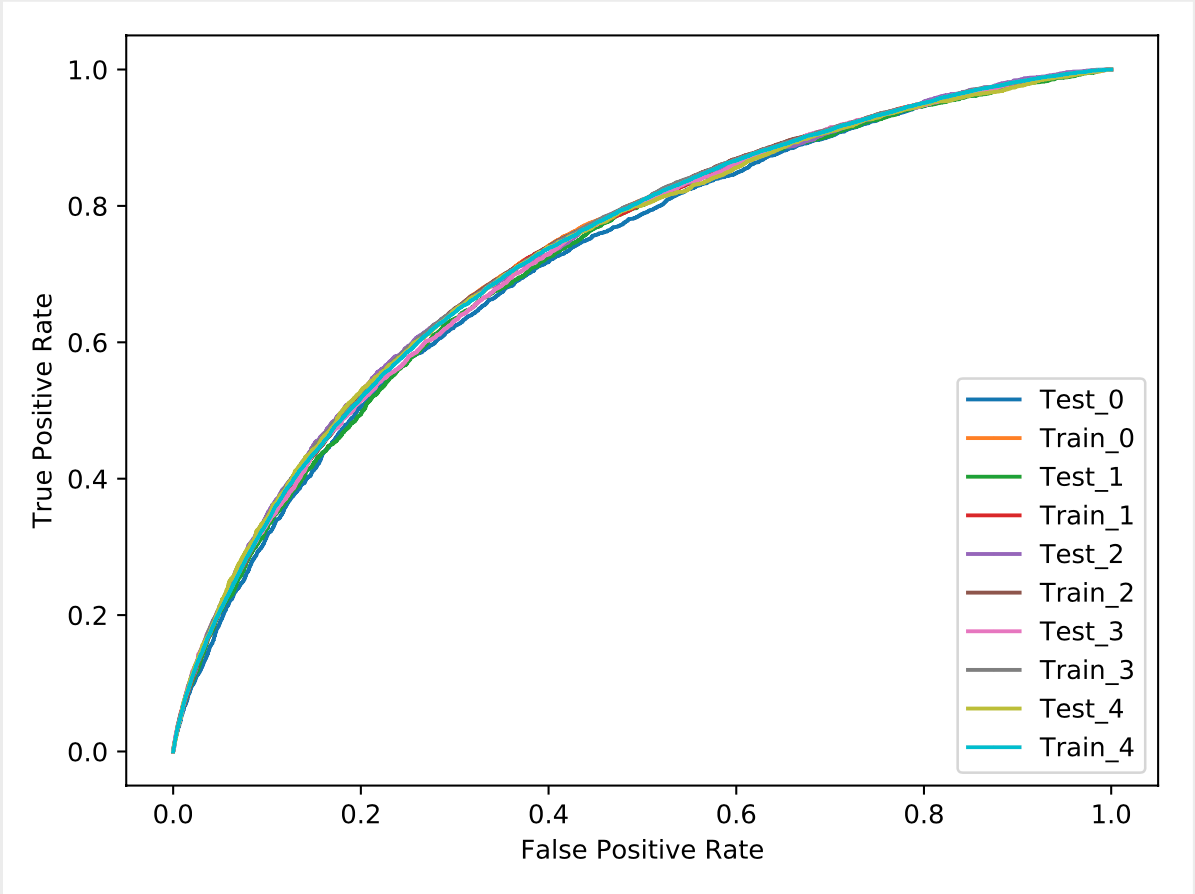
\includegraphics[width=.9\linewidth]{Appendices/BDT/AlternativeModels/SS_ttW/Roc_curve_ttW_SS_LR_003_LowRes}
  \caption{ROC}
  \label{fig:BDT:AltModels:ttWSS:ROC}
\end{subfigure}%
\begin{subfigure}{.5\textwidth}
  \centering
  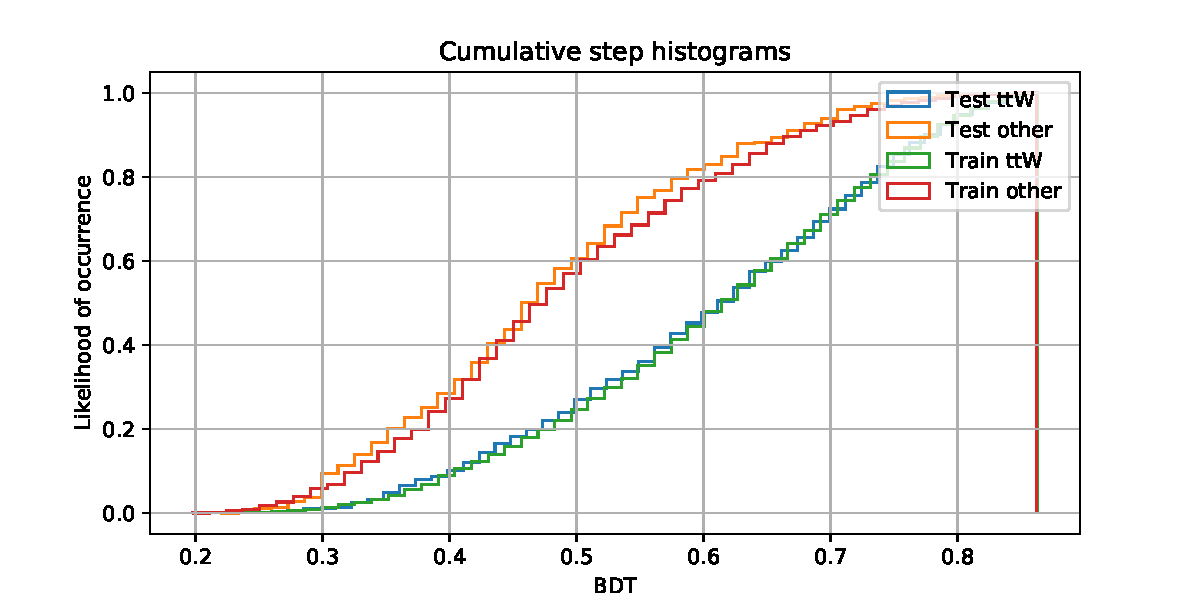
\includegraphics[width=.99\linewidth]{Appendices/BDT/AlternativeModels/SS_ttW/BDT_cumulative_response_ttW_K2_SS_test}
  \caption{Cumulative distribution}
  \label{fig:BDT:AltModels:ttWSS:Score}
\end{subfigure}
\caption{ROC and cumulative distribution of the BDT$(\ttW|_{\text{SS}})$.
The closeness between the orange and blue curves in the cumulative-distribution plot hints
the difficulty to achieve large separations using this model.}
\label{fig:BDT:AltModels:Result:ttWSS}
\end{figure}
\end{comment}



